\documentclass{beamer}

\usepackage{graphicx} % Gestion des images
\usepackage{graphics} % Gestion de placement d'images
\usepackage{hyperref} % Référence liée
\usepackage[english]{babel} % Langue du document
\usepackage[utf8]{inputenc} % Encodage du document
\usepackage[T1]{fontenc} % Encodage de la police
\usepackage[babel=true]{csquotes} % Utilisation d'enquote
\usepackage{tikz}
\usepackage{listings}
\usepackage{amssymb}

% Place with a thick border
\tikzstyle{place}=[circle,thick,draw=blue!75,fill=blue!20,minimum size=6mm]
% Place with a dashed border
\tikzstyle{dplace}=[circle,dashed,draw=blue!75,fill=blue!20,minimum size=6mm]
% White transition style
\tikzstyle{transition}=[rectangle,thick,draw=black!75,
fill=black!20,minimum size=4mm]
% White transition with red border
\tikzstyle{rtransition}=[rectangle,thick,draw=red!75,
fill=white,minimum size=4mm]
% Black transition style
\tikzstyle{btransition}=[rectangle,thick,draw=black!75,
fill=black,minimum size=4mm]
% Black transition with red border
\tikzstyle{rbtransition}=[rectangle,thick,draw=red!75,
fill=black,minimum size=4mm]
% Grey transition style
\tikzstyle{gtransition}=[rectangle,thick,draw=black!75,
fill=black!50!white,minimum size=4mm]

\usetikzlibrary{automata,arrows,positioning,shapes,petri}

\graphicspath{{res/}}

\newenvironment{wideitemize}{\itemize\addtolength{\itemsep}{10pt}}{\enditemize}

\mode<presentation>
	{
	\usetheme{basic}
	%\usetheme{Pittsburgh}
	\setbeamercovered{transparent = 28}
	}

%\usecolortheme{Moo}
%\useinnertheme{Moo}
%\useoutertheme{Moo}


\logo{logo_epl.png}
\title{Semantics for consistent activation in context-oriented systems}
\author{Florian Thuin}
\institute{Ecole Polytechnique de Louvain}
\abrevinstitute{Ecole Polytechnique de Louvain}

\begin{document}


\begin{frame}[plain]
	\titlepage
\end{frame}

\begin{frame}
	\frametitle{Information about the paper}

	\begin{center}
	\textbf{Semantics for consistent activation in context-oriented systems}
	\bigskip


	\href{https://www.researchgate.net/profile/Nicolas_Cardozo}{Nicolás Cardozo}

	\href{https://www.researchgate.net/profile/Sebastian_Gonzalez4}{Sebastián González}

	\href{https://www.researchgate.net/profile/Kim_Mens}{Kim Mens}

	\href{https://www.researchgate.net/profile/Ragnhild_Van_Der_Straeten}{Ragnhild Van Der Straeten}

	\href{https://www.researchgate.net/profile/Jorge_Vallejos}{Jorge Vallejos}

	\href{https://www.researchgate.net/researcher/76177048_Theo_DHondt}{Theo D'Hondt}
	\bigskip

	\textit{October 1, 2014}
	\end{center}

	\bigskip

	Find the full-text PDF at \url{https://www.researchgate.net/publication/267634206}
\end{frame}

\AtBeginSection[]
{
   \begin{frame}
       \frametitle{Plan}
       \tableofcontents[currentsection]
   \end{frame}
}

\section{Introduction}

\begin{frame}
	\frametitle{Introduction}

	\begin{center}
	\enquote{\Large Semantics for consistent activation in context-oriented systems} \newline
	\end{center}

	What I will talk about:

	\begin{itemize}
		\item What is a context ?
		\item What is a context-oriented system ?
		\item How to model \textbf{context (de)activations} ?
		\item How to model \textbf{relations between contexts} ?
	\end{itemize}
\end{frame}

\begin{frame}
	\frametitle{Hardware evolution \& programming techniques}


	\begin{itemize}
		\item Smartphones have a lot of \textit{\textbf{sensors}}, allowing
	programs to interact with their environment.
	\end{itemize}


	\begin{figure}[!ht]
		\centering
	\begin{tikzpicture}
		\node (smartphone) {
\includegraphics[width=0.1\linewidth]{smartphone.png}};
		\node[above left = -0.7cm and 0cm of smartphone] (a) {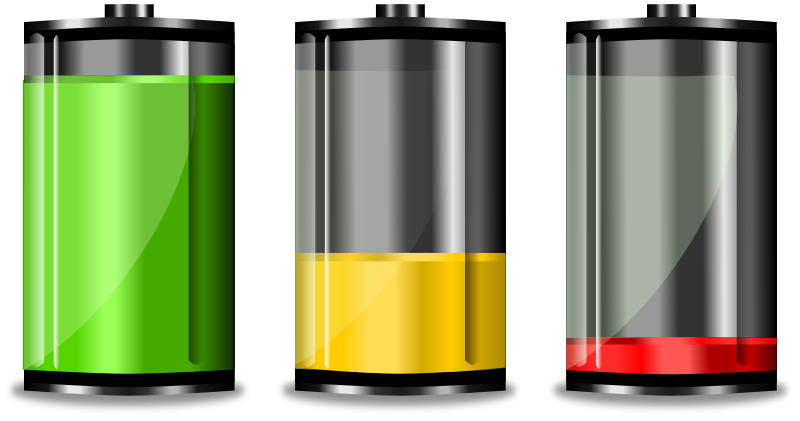
\includegraphics[width=0.1\linewidth]{battery_level.png}};
		\node[below left = -0.75cm and 0cm of smartphone]{
\includegraphics[width=0.05\linewidth]{world.png}};
		\node[above right = -0.75cm and 0cm of smartphone] {
\includegraphics[width=0.05\linewidth]{weather.png}};
		\node[below right = -0.75cm and 0cm of smartphone]{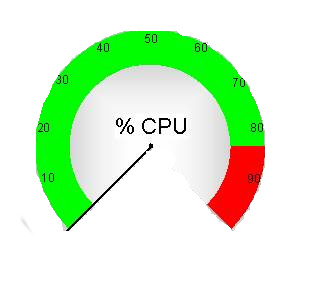
\includegraphics[width=0.05\linewidth]{cpu_load.png}};
	\end{tikzpicture}
	\end{figure}

	\begin{itemize}
		\item You can use them to provide a better user experience
	\end{itemize}

	\begin{figure}[!ht]
		\begin{minipage}{\linewidth}
			\begin{minipage}{0.7\linewidth}
				\begin{itemize}
					\item Most of programming techniques don't provide a reusable
					and maintainable approach to do it
				\end{itemize}
			\end{minipage}
			\begin{minipage}{0.25\linewidth}
				
\includegraphics[width=0.6\linewidth]{computer.png}
				%
\includegraphics[width=\linewidth]{back_in_my_days.png}
			\end{minipage}
		\end{minipage}
	\end{figure}

	\begin{itemize}
		\item Context-oriented programming has been made for this!
	\end{itemize}
\end{frame}

\section{Context-oriented programming}

\begin{frame}
    \frametitle{What is a context?}

    \begin{tikzpicture}
        % Left part
        \node[draw, color=green!50!black] (reallife) at (3,4) {\large \textbf{In real life}};

        \node[anchor=south west, inner sep=0] (smartphone) {
\includegraphics[height=0.3\paperheight]{smartphone.png}};
        \node[above right = 0cm and 1.25cm of smartphone] (LowBattery) {Low battery};
        \path[-] (smartphone.center) edge node {} (LowBattery.west);
        \node[below = 0.5cm of LowBattery] (GeographicalLocation) {Geographical location};
        \path[-] (smartphone.center) edge node {} (GeographicalLocation.west);
        \node[below = 0.5cm of GeographicalLocation] (Weather) {Weather conditions};
        \path[-] (smartphone.center) edge node {} (Weather.west);
        \node[below = 0.5cm of Weather] (HighCPU) {High CPU load};
        \path[-] (smartphone.center) edge node {} (HighCPU.west);

        % Middle line
        \node (a) at (6,4) {};
        \node (b) at (6,-1) {};
        \path[-,dashed, color=red!50!black, line width=2mm] (a) edge node {} (b);
        \node[above = -0.25cm of a, color=red!50!black] {\textbf{Reification}};

        % Right part
        \node[draw, color=green!50!black] (objects) at (8.5,4) {\large \textbf{Objects}};

        \node[right= 2.25cm of LowBattery] (LowBatteryContext) {LowBatteryContext};
        \path[-latex] (LowBattery) edge node {} (LowBatteryContext);
        \node[below= 0.5cm of LowBatteryContext] (GeographicalLocationContext) {GeographicalLocationContext};
        \path[-latex] (GeographicalLocation) edge node {} (GeographicalLocationContext);
        \node[below= 0.5cm of GeographicalLocationContext] (WeatherContext) {WeatherContext};
        \path[-latex] (Weather) edge node {} (WeatherContext);
        \node[below= 0.5cm of WeatherContext] (HighCPUContext) {HighCPUContext};
        \path[-latex] (HighCPU) edge node {} (HighCPUContext);
    \end{tikzpicture}

    \begin{itemize}
    	\item The environment is modelled by contexts that are
    	\begin{itemize}
    		\item active \textit{or}
    		\item inactive
    	\end{itemize}
    	\item This paradigm is called \textbf{context-oriented programming}
    \end{itemize}
\end{frame}

\begin{frame}
    \frametitle{What is a context-oriented system?}

    A context-oriented system:

    \begin{wideitemize}
        \item is implemented with \textbf{context-oriented programming}
        \item has \textbf{Context} abstraction encoded as \textbf{first-class entities}
        \item has a certain number of \textit{active} and \textit{inactive} contexts
        \item has a \textbf{context-specific behavior} (depends on active contexts and their adaptations)
    \end{wideitemize}

\end{frame}

\begin{frame}
	\frametitle{Activation and deactivation of contexts}
	\begin{itemize}
		\item Context can be in 2 states:
		\begin{itemize}
			\item active \textit{or}
			\item inactive
		\end{itemize}
		\item Context becomes active after an \textbf{activation} request
		\item Context becomes inactive after a \textbf{deactivation} request
	\end{itemize}
	\bigskip

	\pause
	$\Rightarrow$ That's nice, but how to \textit{model} it?
\end{frame}

\section{Context modelling}

\begin{frame}
	\frametitle{Petri Net}

	A Petri Net is a graph with \textbf{transitions} and \textbf{places}.

	\begin{itemize}
		\item Transitions are events
		\item Places are conditions
	\end{itemize}

	\begin{figure}[!ht]
	\centering

	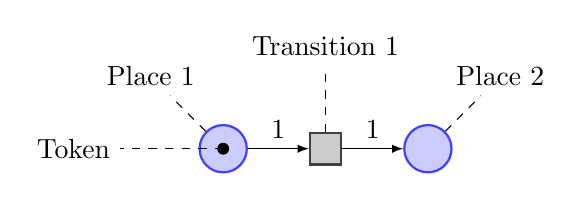
\begin{tikzpicture}[node distance=1.3cm, >=stealth',bend angle=45,auto]
		\tikzstyle{place}=[circle,thick,draw=blue!75,fill=blue!20,minimum size=6mm]
  \tikzstyle{red place}=[place,draw=red!75,fill=red!20]
  \tikzstyle{transition}=[rectangle,thick,draw=black!75,
  			  fill=black!20,minimum size=4mm]

  		\node[place,tokens=1] (a) {};
  		\node[above left of=a] (place1) {Place 1};
  		\path[-,dashed] (a) edge node {} (place1);
  		\node[left = 1cm of a] (token) {Token};
  		\path[-,dashed] (a.center) edge node {} (token);
  		\node[transition, right of=a] (b) {};
  		\node[above of=b] (transition) {Transition 1};
  		\path[-,dashed] (b) edge node {} (transition);
  		\path[-latex] (a) edge node {1} (b);
  		\node[place, right of=b] (c) {};
  		\path[-latex] (b) edge node {1} (c);
  		\node[above right of=c] (place2) {Place 2};
  		\path[-,dashed] (c) edge node {} (place2);
	\end{tikzpicture}

	\end{figure}

	\pause

	A transition can be \textbf{fired} if there are sufficient tokens in its input places.

	\begin{figure}[!ht]
	\centering

	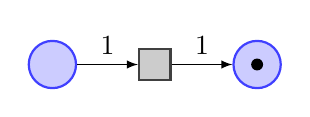
\begin{tikzpicture}[node distance=1.3cm, >=stealth',bend angle=45,auto]
		\tikzstyle{place}=[circle,thick,draw=blue!75,fill=blue!20,minimum size=6mm]
  \tikzstyle{red place}=[place,draw=red!75,fill=red!20]
  \tikzstyle{transition}=[rectangle,thick,draw=black!75,
  			  fill=black!20,minimum size=4mm]

  		\node[place] (a) {};
  		\node[transition, right of=a] (b) {};
  		\path[-latex] (a) edge node {1} (b);
  		\node[place, right of=b, tokens=1] (c) {};
  		\path[-latex] (b) edge node {1} (c);
	\end{tikzpicture}

	\end{figure}
\end{frame}

\begin{frame}
	\frametitle{Why Petri Nets?}

	\begin{wideitemize}
		\item Petri Nets are good at modelling:

		\begin{wideitemize}
			\item Choices
			\item Iteration
			\item Concurrent execution
			\item Multiple activations (more than one token in a place)
		\end{wideitemize}

		\item They have nice properties, such as:

		\begin{wideitemize}
			\item Coverability
			\item Reachability
			\item Liveness
		\end{wideitemize}
	\end{wideitemize}

	\pause

	$\Rightarrow$ Those properties can be used to \textbf{identify conflicts}!
\end{frame}

\begin{frame}
	\frametitle{Petri Net limitation}

	\begin{exampleblock}{Property}
	COP systems must ensure the \textbf{reactivity} to changes in the surrounding execution environment.
	\end{exampleblock}
	\bigskip

	 Reactive systems have \textit{perfect-synchrony hypothesis}:
	\begin{itemize}
		\item Outputs are produced instantaneously after the inputs occur.
	\end{itemize}

	\bigskip
	\pause
	\begin{alertblock}{Bad news}
		Petri Nets are not expressive enough for this hypothesis\ldots
	\end{alertblock}


\end{frame}

\begin{frame}
	\frametitle{Reactive Petri Net}

	\begin{figure}[!ht]
		
\includegraphics[width=0.3\linewidth]{good_news_everyone.png}
	\end{figure}

	\textbf{Reactive Petri Net} splits transitions into

	\begin{itemize}
		\item \textbf{External} transitions \tikz{\node[transition] {};} that \textbf{may} fire
		\item \textbf{Internal} transitions \tikz{\node[btransition] {};} that \textbf{must} fire
	\end{itemize}

	\begin{figure}[!ht]
	\centering
	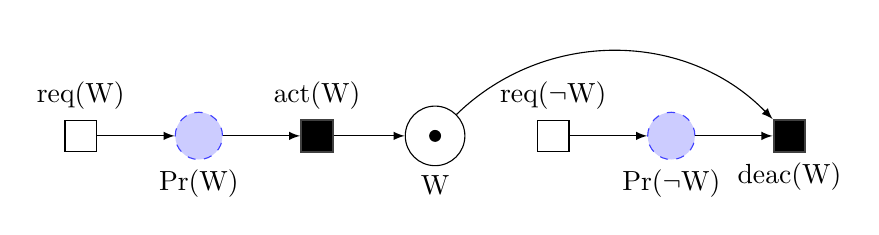
\begin{tikzpicture}[node distance=1.5cm, >=stealth',bend angle=45,auto]
  		\node[transition,label=above:req(W)] (t1) {};
  		\node[dplace, right of=t1,label=below:Pr(W)] (p1) {};
  		\node[btransition, right of=p1,label=above:act(W)] (t2) {};
  		\node[place, right of=t2,label=below:W, tokens=1] (p2) {};
  		\node[transition, right of=p2,label=above:req($\lnot$W)] (t3) {};
  		\node[dplace, right of=t3,label=below:Pr($\lnot$W)] (p3) {};
  		\node[btransition, right of=p3,label=below:deac(W)] (t4) {};

  		\path[-latex] (t1) edge node {} (p1);
  		\path[-latex] (p1) edge node {} (t2);
  		\path[-latex] (t2) edge node {} (p2);
  		\path[-latex] (p2) edge[bend left=45] node {} (t4);
  		\path[-latex] (t3) edge node {} (p3);
  		\path[-latex] (p3) edge node {} (t4);

	\end{tikzpicture}
	\caption{Example of a \texttt{WiFi} (W) context (de)activation Petri Net}
	\end{figure}
\end{frame}

\begin{frame}
	\frametitle{Relation between contexts}

	A context-oriented system has \textbf{multiple} contexts.
	\bigskip

	Contexts can be related to each others.
	\bigskip

	\textbf{Example} A system with 3 contexts:

	\begin{itemize}
		\item WiFi context (W)
		\item 3G context (3G)
		\item Connectivity context (C)
	\end{itemize}
	\pause

	If WiFi is enabled or 3G is enabled, the connectivity must be enabled
	too.

	\pause
	\bigskip
	This is called a \textbf{disjunction dependency relation}.

\end{frame}

\begin{frame}[plain]
    \begin{figure}[!ht]
        \centering
        \scriptsize
        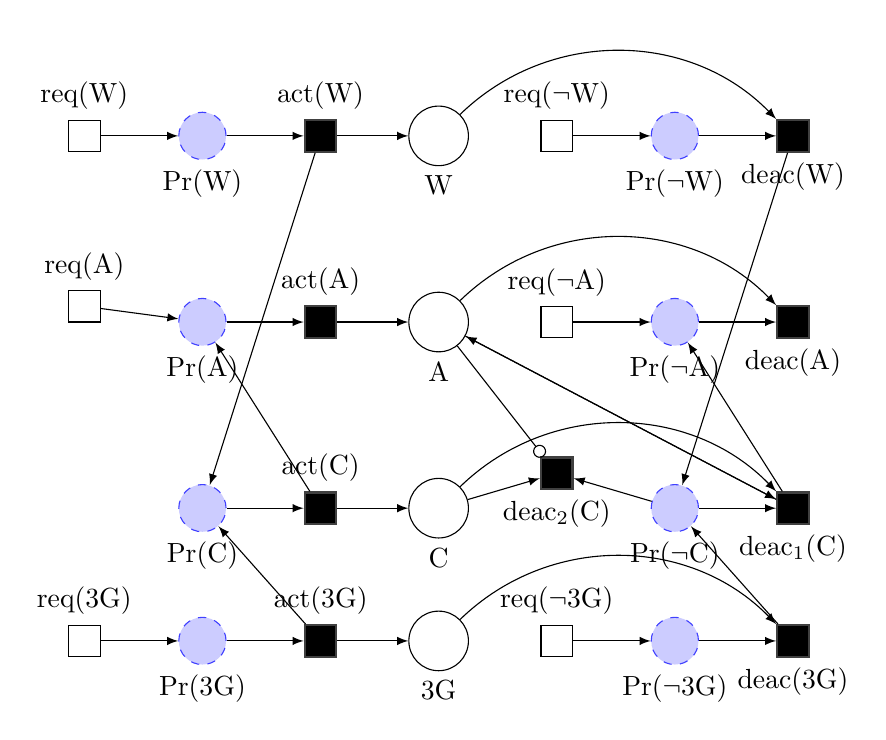
\begin{tikzpicture}[node distance=1.5cm, >=stealth',bend angle=45,auto]
            % WiFi PART

            \node[transition,									label=above:req(W)] (t1) {};
            \node[dplace,right of=t1,tokens=0,label=below:Pr(W)] (p1) {};
            \node[btransition, right of=p1,		label=above:act(W)] (t2) {};
            \node[place, right of=t2,tokens=0,label=below:W] (p2) {};
            \node[transition, right of=p2,		label=above:req($\lnot$W)] (t3) {};
            \node[dplace,right of=t3,tokens=0,label=below:Pr($\lnot$W)] (p3) {};
            \node[btransition, right of=p3,		label=below:deac(W)] (t4) {};

            \path[-latex] (t1) edge node {} (p1);
            \path[-latex] (p1) edge node {} (t2);
            \path[-latex] (t2) edge node {} (p2);
            \path[-latex] (p2) edge[bend left=45] node {} (t4);
            \path[-latex] (t3) edge node {} (p3);
            \path[-latex] (p3) edge node {} (t4);


            % AudioStream PART

            \node[transition,below =1.75cm of t1,  label=above:req(A)] (t13) {};
            \node[dplace, below = 1.75cm of p1,    label=below:Pr(A)] (p10) {};
            \node[btransition, right of=p10,    label=above:act(A)] (t14) {};
            \node[place, right of=t14,tokens=0, label=below:A] (p11) {};
            \node[transition, right of=p11,		label=above:req($\lnot$A)] (t15) {};
            \node[dplace, below =1.75cm of p3,     label=below:Pr($\lnot$A)] (p12) {};
            \node[btransition, right of=p12,    label=below:deac(A)] (t16) {};

            \path[-latex] (t13) edge node {} (p10);
            \path[-latex] (p10) edge node {} (t14);
            \path[-latex] (t14) edge node {} (p11);
            \path[-latex] (p11) edge[bend left=45] node {} (t16);
            \path[-latex] (t15) edge node {} (p12);
            \path[-latex] (p12) edge node {} (t16);

            % Connectivity PART

            %\node[transition,below =2cm of t1,	label=above:req(C)] (t9) {};
            \node[dplace, below = 1.75cm of p10,					label=below:Pr(C)] (p7) {};
            \node[btransition, right of=p7,			label=above:act(C)] (t10) {};
            \node[place, right of=t10,tokens=0,	label=below:C] (p8) {};
            %\node[transition, right of=p8,			label=above:req($\lnot$C)] (t11) {};
            \node[dplace, below =1.75cm of p12,					label=below:Pr($\lnot$C)] (p9) {};
            \node[btransition, right of=p9,			label=below:deac$_1$(C)] (t12) {};
            \node[btransition, below=1.5cm of t15,     label=below:deac$_2$(C)] (t17) {};

            %\path[-latex] (t9) edge node {} (p7);
            \path[-latex] (p7) edge node {} (t10);
            \path[-latex] (t10) edge node {} (p8);
            \path[-latex] (p8) edge[bend left=45] node {} (t12);
            %\path[-latex] (t11) edge node {} (p9);
            \path[-latex] (p9) edge node {} (t12);

            % 3G PART

            \node[transition,below =6cm of t1,	label=above:req(3G)] (t5) {};
            \node[dplace, right of=t5,					label=below:Pr(3G)] (p4) {};
            \node[btransition, right of=p4,			label=above:act(3G)] (t6) {};
            \node[place, right of=t6,tokens=0,	label=below:3G] (p5) {};
            \node[transition, right of=p5,			label=above:req($\lnot$3G)] (t7) {};
            \node[dplace, right of=t7,					label=below:Pr($\lnot$3G)] (p6) {};
            \node[btransition, right of=p6,			label=below:deac(3G)] (t8) {};

            \path[-latex] (t5) edge node {} (p4);
            \path[-latex] (p4) edge node {} (t6);
            \path[-latex] (t6) edge node {} (p5);
            \path[-latex] (p5) edge[bend left=45] node {} (t8);
            \path[-latex] (t7) edge node {} (p6);
            \path[-latex] (p6) edge node {} (t8);

            % Connections of Contexts

            \path[-latex] (t2) edge node {} (p7);
            \path[-latex] (t6) edge node {} (p7);
            \path[-latex] (t4) edge node {} (p9);
            \path[-latex] (t8) edge node {} (p9);


            % Connections of Contexts

            \path[-latex] (t10) edge node {} (p10);
            \path[-latex] (t12) edge node {} (p11);
            \path[-latex] (p11) edge node {} (t12);
            \path[-latex] (t12) edge node {} (p12);
            \path[-latex] (p8) edge node {} (t17);
            \path[-latex] (p9) edge node {} (t17);

            \path[-o] (p11) edge node {} (t17);

        \end{tikzpicture}
    \end{figure}
\end{frame}


\begin{frame}[noframenumbering,plain]
    \begin{figure}[!ht]
        \centering
        \scriptsize
        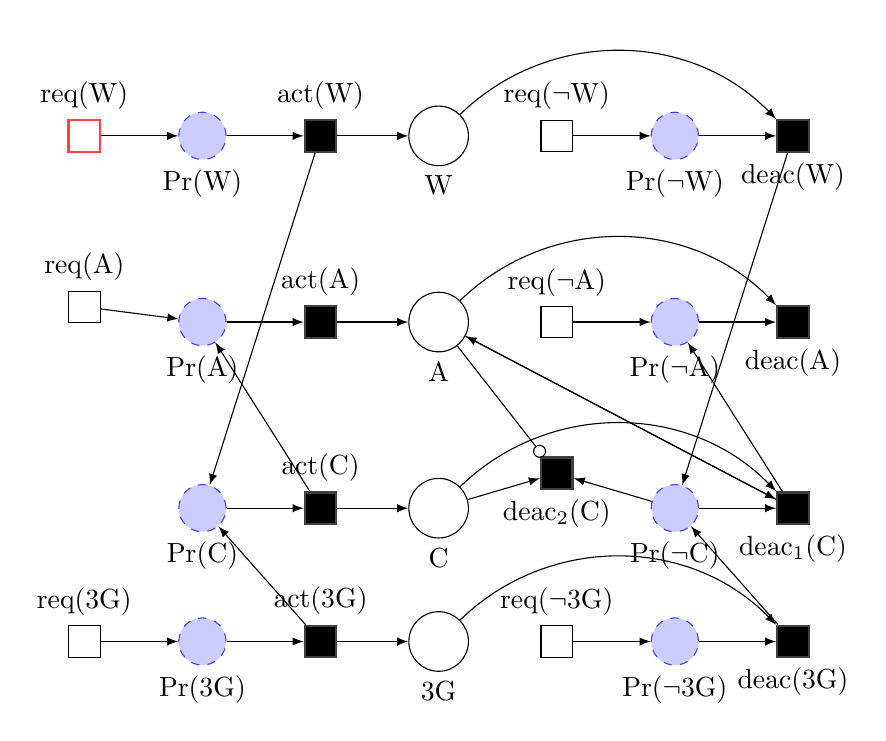
\begin{tikzpicture}[node distance=1.5cm, >=stealth',bend angle=45,auto]
            % WiFi PART

            \node[rtransition,									label=above:req(W)] (t1) {};
            \node[dplace,right of=t1,tokens=0,label=below:Pr(W)] (p1) {};
            \node[btransition, right of=p1,		label=above:act(W)] (t2) {};
            \node[place, right of=t2,tokens=0,label=below:W] (p2) {};
            \node[transition, right of=p2,		label=above:req($\lnot$W)] (t3) {};
            \node[dplace,right of=t3,tokens=0,label=below:Pr($\lnot$W)] (p3) {};
            \node[btransition, right of=p3,		label=below:deac(W)] (t4) {};

            \path[-latex] (t1) edge node {} (p1);
            \path[-latex] (p1) edge node {} (t2);
            \path[-latex] (t2) edge node {} (p2);
            \path[-latex] (p2) edge[bend left=45] node {} (t4);
            \path[-latex] (t3) edge node {} (p3);
            \path[-latex] (p3) edge node {} (t4);


            % AudioStream PART

            \node[transition,below =1.75cm of t1,  label=above:req(A)] (t13) {};
            \node[dplace, below = 1.75cm of p1,    label=below:Pr(A)] (p10) {};
            \node[btransition, right of=p10,    label=above:act(A)] (t14) {};
            \node[place, right of=t14,tokens=0, label=below:A] (p11) {};
            \node[transition, right of=p11,		label=above:req($\lnot$A)] (t15) {};
            \node[dplace, below =1.75cm of p3,     label=below:Pr($\lnot$A)] (p12) {};
            \node[btransition, right of=p12,    label=below:deac(A)] (t16) {};

            \path[-latex] (t13) edge node {} (p10);
            \path[-latex] (p10) edge node {} (t14);
            \path[-latex] (t14) edge node {} (p11);
            \path[-latex] (p11) edge[bend left=45] node {} (t16);
            \path[-latex] (t15) edge node {} (p12);
            \path[-latex] (p12) edge node {} (t16);

            % Connectivity PART

            %\node[transition,below =2cm of t1,	label=above:req(C)] (t9) {};
            \node[dplace, below = 1.75cm of p10,					label=below:Pr(C)] (p7) {};
            \node[btransition, right of=p7,			label=above:act(C)] (t10) {};
            \node[place, right of=t10,tokens=0,	label=below:C] (p8) {};
            %\node[transition, right of=p8,			label=above:req($\lnot$C)] (t11) {};
            \node[dplace, below =1.75cm of p12,					label=below:Pr($\lnot$C)] (p9) {};
            \node[btransition, right of=p9,			label=below:deac$_1$(C)] (t12) {};
            \node[btransition, below=1.5cm of t15,     label=below:deac$_2$(C)] (t17) {};

            %\path[-latex] (t9) edge node {} (p7);
            \path[-latex] (p7) edge node {} (t10);
            \path[-latex] (t10) edge node {} (p8);
            \path[-latex] (p8) edge[bend left=45] node {} (t12);
            %\path[-latex] (t11) edge node {} (p9);
            \path[-latex] (p9) edge node {} (t12);

            % 3G PART

            \node[transition,below =6cm of t1,	label=above:req(3G)] (t5) {};
            \node[dplace, right of=t5,					label=below:Pr(3G)] (p4) {};
            \node[btransition, right of=p4,			label=above:act(3G)] (t6) {};
            \node[place, right of=t6,tokens=0,	label=below:3G] (p5) {};
            \node[transition, right of=p5,			label=above:req($\lnot$3G)] (t7) {};
            \node[dplace, right of=t7,					label=below:Pr($\lnot$3G)] (p6) {};
            \node[btransition, right of=p6,			label=below:deac(3G)] (t8) {};

            \path[-latex] (t5) edge node {} (p4);
            \path[-latex] (p4) edge node {} (t6);
            \path[-latex] (t6) edge node {} (p5);
            \path[-latex] (p5) edge[bend left=45] node {} (t8);
            \path[-latex] (t7) edge node {} (p6);
            \path[-latex] (p6) edge node {} (t8);

            % Connections of Contexts

            \path[-latex] (t2) edge node {} (p7);
            \path[-latex] (t6) edge node {} (p7);
            \path[-latex] (t4) edge node {} (p9);
            \path[-latex] (t8) edge node {} (p9);


            % Connections of Contexts

            \path[-latex] (t10) edge node {} (p10);
            \path[-latex] (t12) edge node {} (p11);
            \path[-latex] (p11) edge node {} (t12);
            \path[-latex] (t12) edge node {} (p12);
            \path[-latex] (p8) edge node {} (t17);
            \path[-latex] (p9) edge node {} (t17);

            \path[-o] (p11) edge node {} (t17);

        \end{tikzpicture}
    \end{figure}
\end{frame}


\begin{frame}[noframenumbering,plain]
    \begin{figure}[!ht]
        \centering
        \scriptsize
        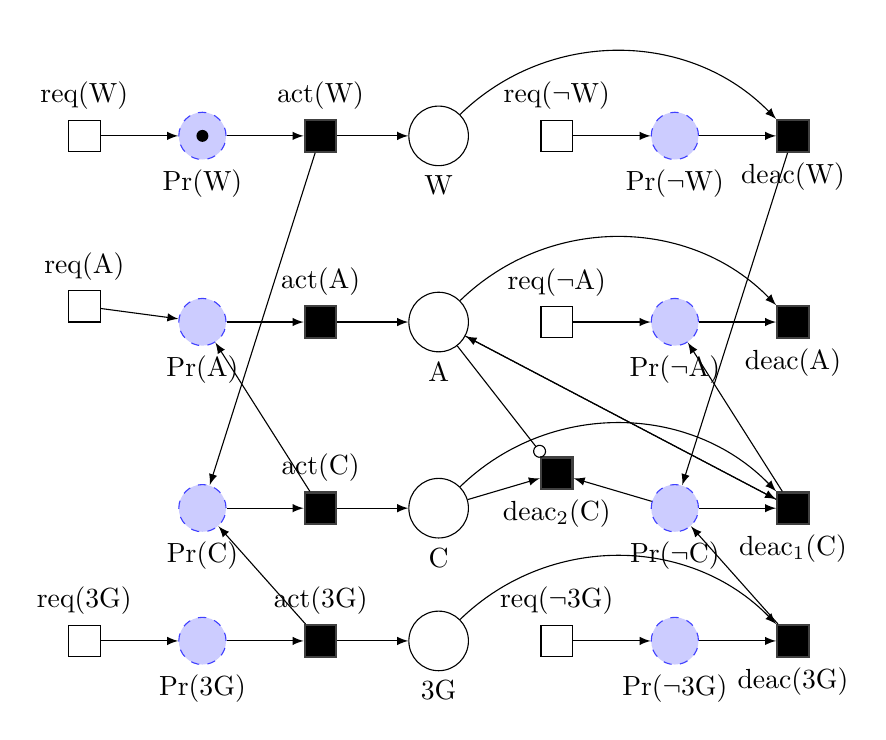
\begin{tikzpicture}[node distance=1.5cm, >=stealth',bend angle=45,auto]
            % WiFi PART

            \node[transition,									label=above:req(W)] (t1) {};
            \node[dplace,right of=t1,tokens=1,label=below:Pr(W)] (p1) {};
            \node[btransition, right of=p1,		label=above:act(W)] (t2) {};
            \node[place, right of=t2,tokens=0,label=below:W] (p2) {};
            \node[transition, right of=p2,		label=above:req($\lnot$W)] (t3) {};
            \node[dplace,right of=t3,tokens=0,label=below:Pr($\lnot$W)] (p3) {};
            \node[btransition, right of=p3,		label=below:deac(W)] (t4) {};

            \path[-latex] (t1) edge node {} (p1);
            \path[-latex] (p1) edge node {} (t2);
            \path[-latex] (t2) edge node {} (p2);
            \path[-latex] (p2) edge[bend left=45] node {} (t4);
            \path[-latex] (t3) edge node {} (p3);
            \path[-latex] (p3) edge node {} (t4);


            % AudioStream PART

            \node[transition,below =1.75cm of t1,  label=above:req(A)] (t13) {};
            \node[dplace, below = 1.75cm of p1,    label=below:Pr(A)] (p10) {};
            \node[btransition, right of=p10,    label=above:act(A)] (t14) {};
            \node[place, right of=t14,tokens=0, label=below:A] (p11) {};
            \node[transition, right of=p11,		label=above:req($\lnot$A)] (t15) {};
            \node[dplace, below =1.75cm of p3,     label=below:Pr($\lnot$A)] (p12) {};
            \node[btransition, right of=p12,    label=below:deac(A)] (t16) {};

            \path[-latex] (t13) edge node {} (p10);
            \path[-latex] (p10) edge node {} (t14);
            \path[-latex] (t14) edge node {} (p11);
            \path[-latex] (p11) edge[bend left=45] node {} (t16);
            \path[-latex] (t15) edge node {} (p12);
            \path[-latex] (p12) edge node {} (t16);

            % Connectivity PART

            %\node[transition,below =2cm of t1,	label=above:req(C)] (t9) {};
            \node[dplace, below = 1.75cm of p10,					label=below:Pr(C)] (p7) {};
            \node[btransition, right of=p7,			label=above:act(C)] (t10) {};
            \node[place, right of=t10,tokens=0,	label=below:C] (p8) {};
            %\node[transition, right of=p8,			label=above:req($\lnot$C)] (t11) {};
            \node[dplace, below =1.75cm of p12,					label=below:Pr($\lnot$C)] (p9) {};
            \node[btransition, right of=p9,			label=below:deac$_1$(C)] (t12) {};
            \node[btransition, below=1.5cm of t15,     label=below:deac$_2$(C)] (t17) {};

            %\path[-latex] (t9) edge node {} (p7);
            \path[-latex] (p7) edge node {} (t10);
            \path[-latex] (t10) edge node {} (p8);
            \path[-latex] (p8) edge[bend left=45] node {} (t12);
            %\path[-latex] (t11) edge node {} (p9);
            \path[-latex] (p9) edge node {} (t12);

            % 3G PART

            \node[transition,below =6cm of t1,	label=above:req(3G)] (t5) {};
            \node[dplace, right of=t5,					label=below:Pr(3G)] (p4) {};
            \node[btransition, right of=p4,			label=above:act(3G)] (t6) {};
            \node[place, right of=t6,tokens=0,	label=below:3G] (p5) {};
            \node[transition, right of=p5,			label=above:req($\lnot$3G)] (t7) {};
            \node[dplace, right of=t7,					label=below:Pr($\lnot$3G)] (p6) {};
            \node[btransition, right of=p6,			label=below:deac(3G)] (t8) {};

            \path[-latex] (t5) edge node {} (p4);
            \path[-latex] (p4) edge node {} (t6);
            \path[-latex] (t6) edge node {} (p5);
            \path[-latex] (p5) edge[bend left=45] node {} (t8);
            \path[-latex] (t7) edge node {} (p6);
            \path[-latex] (p6) edge node {} (t8);

            % Connections of Contexts

            \path[-latex] (t2) edge node {} (p7);
            \path[-latex] (t6) edge node {} (p7);
            \path[-latex] (t4) edge node {} (p9);
            \path[-latex] (t8) edge node {} (p9);


            % Connections of Contexts

            \path[-latex] (t10) edge node {} (p10);
            \path[-latex] (t12) edge node {} (p11);
            \path[-latex] (p11) edge node {} (t12);
            \path[-latex] (t12) edge node {} (p12);
            \path[-latex] (p8) edge node {} (t17);
            \path[-latex] (p9) edge node {} (t17);

            \path[-o] (p11) edge node {} (t17);

        \end{tikzpicture}
    \end{figure}
\end{frame}


\begin{frame}[noframenumbering,plain]
    \begin{figure}[!ht]
        \centering
        \scriptsize
        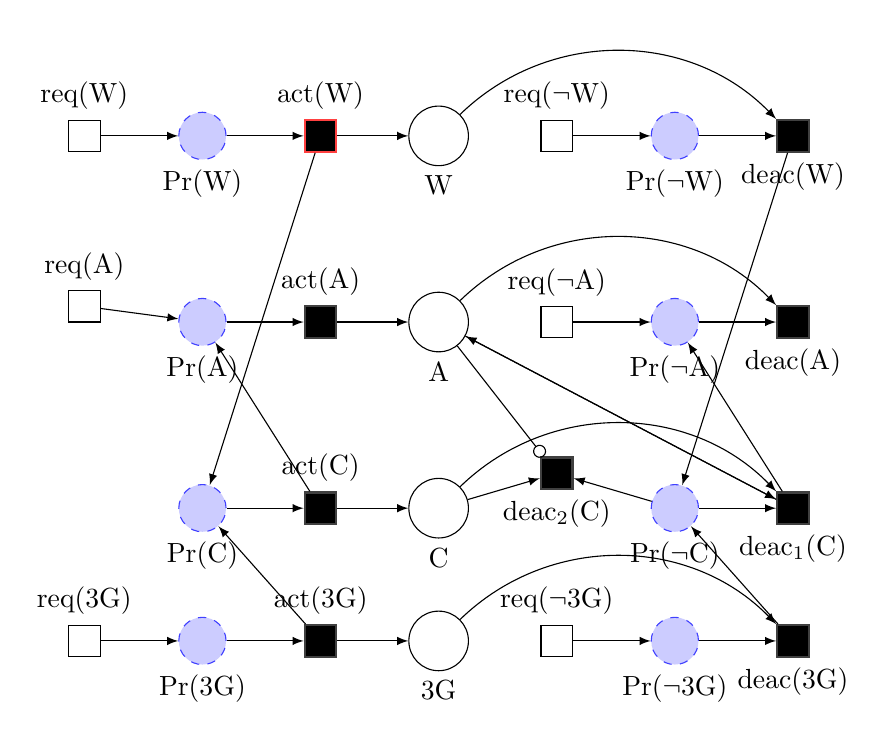
\begin{tikzpicture}[node distance=1.5cm, >=stealth',bend angle=45,auto]
            % WiFi PART

            \node[transition,									label=above:req(W)] (t1) {};
            \node[dplace,right of=t1,tokens=0,label=below:Pr(W)] (p1) {};
            \node[rbtransition, right of=p1,		label=above:act(W)] (t2) {};
            \node[place, right of=t2,tokens=0,label=below:W] (p2) {};
            \node[transition, right of=p2,		label=above:req($\lnot$W)] (t3) {};
            \node[dplace,right of=t3,tokens=0,label=below:Pr($\lnot$W)] (p3) {};
            \node[btransition, right of=p3,		label=below:deac(W)] (t4) {};

            \path[-latex] (t1) edge node {} (p1);
            \path[-latex] (p1) edge node {} (t2);
            \path[-latex] (t2) edge node {} (p2);
            \path[-latex] (p2) edge[bend left=45] node {} (t4);
            \path[-latex] (t3) edge node {} (p3);
            \path[-latex] (p3) edge node {} (t4);


            % AudioStream PART

            \node[transition,below =1.75cm of t1,  label=above:req(A)] (t13) {};
            \node[dplace, below = 1.75cm of p1,    label=below:Pr(A)] (p10) {};
            \node[btransition, right of=p10,    label=above:act(A)] (t14) {};
            \node[place, right of=t14,tokens=0, label=below:A] (p11) {};
            \node[transition, right of=p11,		label=above:req($\lnot$A)] (t15) {};
            \node[dplace, below =1.75cm of p3,     label=below:Pr($\lnot$A)] (p12) {};
            \node[btransition, right of=p12,    label=below:deac(A)] (t16) {};

            \path[-latex] (t13) edge node {} (p10);
            \path[-latex] (p10) edge node {} (t14);
            \path[-latex] (t14) edge node {} (p11);
            \path[-latex] (p11) edge[bend left=45] node {} (t16);
            \path[-latex] (t15) edge node {} (p12);
            \path[-latex] (p12) edge node {} (t16);

            % Connectivity PART

            %\node[transition,below =2cm of t1,	label=above:req(C)] (t9) {};
            \node[dplace, below = 1.75cm of p10,					label=below:Pr(C)] (p7) {};
            \node[btransition, right of=p7,			label=above:act(C)] (t10) {};
            \node[place, right of=t10,tokens=0,	label=below:C] (p8) {};
            %\node[transition, right of=p8,			label=above:req($\lnot$C)] (t11) {};
            \node[dplace, below =1.75cm of p12,					label=below:Pr($\lnot$C)] (p9) {};
            \node[btransition, right of=p9,			label=below:deac$_1$(C)] (t12) {};
            \node[btransition, below=1.5cm of t15,     label=below:deac$_2$(C)] (t17) {};

            %\path[-latex] (t9) edge node {} (p7);
            \path[-latex] (p7) edge node {} (t10);
            \path[-latex] (t10) edge node {} (p8);
            \path[-latex] (p8) edge[bend left=45] node {} (t12);
            %\path[-latex] (t11) edge node {} (p9);
            \path[-latex] (p9) edge node {} (t12);

            % 3G PART

            \node[transition,below =6cm of t1,	label=above:req(3G)] (t5) {};
            \node[dplace, right of=t5,					label=below:Pr(3G)] (p4) {};
            \node[btransition, right of=p4,			label=above:act(3G)] (t6) {};
            \node[place, right of=t6,tokens=0,	label=below:3G] (p5) {};
            \node[transition, right of=p5,			label=above:req($\lnot$3G)] (t7) {};
            \node[dplace, right of=t7,					label=below:Pr($\lnot$3G)] (p6) {};
            \node[btransition, right of=p6,			label=below:deac(3G)] (t8) {};

            \path[-latex] (t5) edge node {} (p4);
            \path[-latex] (p4) edge node {} (t6);
            \path[-latex] (t6) edge node {} (p5);
            \path[-latex] (p5) edge[bend left=45] node {} (t8);
            \path[-latex] (t7) edge node {} (p6);
            \path[-latex] (p6) edge node {} (t8);

            % Connections of Contexts

            \path[-latex] (t2) edge node {} (p7);
            \path[-latex] (t6) edge node {} (p7);
            \path[-latex] (t4) edge node {} (p9);
            \path[-latex] (t8) edge node {} (p9);


            % Connections of Contexts

            \path[-latex] (t10) edge node {} (p10);
            \path[-latex] (t12) edge node {} (p11);
            \path[-latex] (p11) edge node {} (t12);
            \path[-latex] (t12) edge node {} (p12);
            \path[-latex] (p8) edge node {} (t17);
            \path[-latex] (p9) edge node {} (t17);

            \path[-o] (p11) edge node {} (t17);

        \end{tikzpicture}
    \end{figure}
\end{frame}


\begin{frame}[noframenumbering]
    \frametitle{Relation between contexts}
    \begin{figure}[!ht]
        \centering
        \scriptsize
        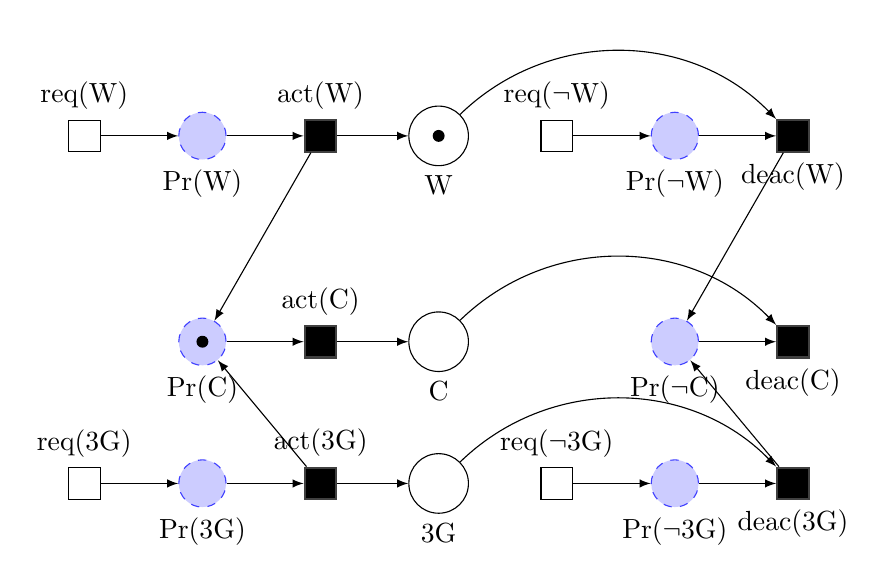
\begin{tikzpicture}[node distance=1.5cm, >=stealth',bend angle=45,auto]
            % WiFi PART

            \node[transition,									label=above:req(W)] (t1) {};
            \node[dplace,right of=t1,tokens=0,label=below:Pr(W)] (p1) {};
            \node[btransition, right of=p1,		label=above:act(W)] (t2) {};
            \node[place, right of=t2,tokens=1,label=below:W] (p2) {};
            \node[transition, right of=p2,		label=above:req($\lnot$W)] (t3) {};
            \node[dplace,right of=t3,tokens=0,label=below:Pr($\lnot$W)] (p3) {};
            \node[btransition, right of=p3,		label=below:deac(W)] (t4) {};

            \path[-latex] (t1) edge node {} (p1);
            \path[-latex] (p1) edge node {} (t2);
            \path[-latex] (t2) edge node {} (p2);
            \path[-latex] (p2) edge[bend left=45] node {} (t4);
            \path[-latex] (t3) edge node {} (p3);
            \path[-latex] (p3) edge node {} (t4);

            % 3G PART

            \node[transition,below =4cm of t1,	label=above:req(3G)] (t5) {};
            \node[dplace, right of=t5,					label=below:Pr(3G)] (p4) {};
            \node[btransition, right of=p4,			label=above:act(3G)] (t6) {};
            \node[place, right of=t6,tokens=0,	label=below:3G] (p5) {};
            \node[transition, right of=p5,			label=above:req($\lnot$3G)] (t7) {};
            \node[dplace, right of=t7,					label=below:Pr($\lnot$3G)] (p6) {};
            \node[btransition, right of=p6,			label=below:deac(3G)] (t8) {};

            \path[-latex] (t5) edge node {} (p4);
            \path[-latex] (p4) edge node {} (t6);
            \path[-latex] (t6) edge node {} (p5);
            \path[-latex] (p5) edge[bend left=45] node {} (t8);
            \path[-latex] (t7) edge node {} (p6);
            \path[-latex] (p6) edge node {} (t8);

            % Connectivity PART

            %\node[transition,below =2cm of t1,	label=above:req(C)] (t9) {};
            \node[dplace,below=2cm of p1,tokens=1,label=below:Pr(C)] (p7) {};
            \node[btransition, right of=p7,			label=above:act(C)] (t10) {};
            \node[place, right of=t10,tokens=0,	label=below:C] (p8) {};
            %\node[transition, right of=p8,			label=above:req($\lnot$C)] (t11) {};
            \node[dplace, below =2cm of p3,					label=below:Pr($\lnot$C)] (p9) {};
            \node[btransition, right of=p9,			label=below:deac(C)] (t12) {};

            %\path[-latex] (t9) edge node {} (p7);
            \path[-latex] (p7) edge node {} (t10);
            \path[-latex] (t10) edge node {} (p8);
            \path[-latex] (p8) edge[bend left=45] node {} (t12);
            %\path[-latex] (t11) edge node {} (p9);
            \path[-latex] (p9) edge node {} (t12);

            % Connections of Contexts

            \path[-latex] (t2) edge node {} (p7);
            \path[-latex] (t6) edge node {} (p7);
            \path[-latex] (t4) edge node {} (p9);
            \path[-latex] (t8) edge node {} (p9);

        \end{tikzpicture}
    \end{figure}
\end{frame}


\begin{frame}[noframenumbering]
    \frametitle{Relation between contexts}
    \begin{figure}[!ht]
        \centering
        \scriptsize
        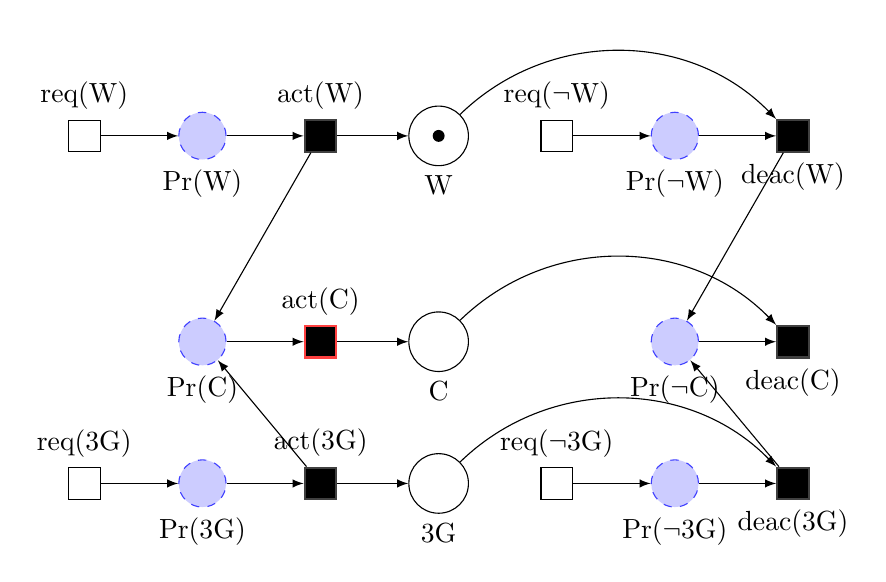
\begin{tikzpicture}[node distance=1.5cm, >=stealth',bend angle=45,auto]
            % WiFi PART

            \node[transition,									label=above:req(W)] (t1) {};
            \node[dplace,right of=t1,tokens=0,label=below:Pr(W)] (p1) {};
            \node[btransition, right of=p1,		label=above:act(W)] (t2) {};
            \node[place, right of=t2,tokens=1,label=below:W] (p2) {};
            \node[transition, right of=p2,		label=above:req($\lnot$W)] (t3) {};
            \node[dplace,right of=t3,tokens=0,label=below:Pr($\lnot$W)] (p3) {};
            \node[btransition, right of=p3,		label=below:deac(W)] (t4) {};

            \path[-latex] (t1) edge node {} (p1);
            \path[-latex] (p1) edge node {} (t2);
            \path[-latex] (t2) edge node {} (p2);
            \path[-latex] (p2) edge[bend left=45] node {} (t4);
            \path[-latex] (t3) edge node {} (p3);
            \path[-latex] (p3) edge node {} (t4);

            % 3G PART

            \node[transition,below =4cm of t1,	label=above:req(3G)] (t5) {};
            \node[dplace, right of=t5,					label=below:Pr(3G)] (p4) {};
            \node[btransition, right of=p4,			label=above:act(3G)] (t6) {};
            \node[place, right of=t6,tokens=0,	label=below:3G] (p5) {};
            \node[transition, right of=p5,			label=above:req($\lnot$3G)] (t7) {};
            \node[dplace, right of=t7,					label=below:Pr($\lnot$3G)] (p6) {};
            \node[btransition, right of=p6,			label=below:deac(3G)] (t8) {};

            \path[-latex] (t5) edge node {} (p4);
            \path[-latex] (p4) edge node {} (t6);
            \path[-latex] (t6) edge node {} (p5);
            \path[-latex] (p5) edge[bend left=45] node {} (t8);
            \path[-latex] (t7) edge node {} (p6);
            \path[-latex] (p6) edge node {} (t8);

            % Connectivity PART

            %\node[transition,below =2cm of t1,	label=above:req(C)] (t9) {};
            \node[dplace, below = 2cm of p1,					label=below:Pr(C)] (p7) {};
            \node[rbtransition, right of=p7,			label=above:act(C)] (t10) {};
            \node[place, right of=t10,tokens=0,	label=below:C] (p8) {};
            %\node[transition, right of=p8,			label=above:req($\lnot$C)] (t11) {};
            \node[dplace, below =2cm of p3,					label=below:Pr($\lnot$C)] (p9) {};
            \node[btransition, right of=p9,			label=below:deac(C)] (t12) {};

            %\path[-latex] (t9) edge node {} (p7);
            \path[-latex] (p7) edge node {} (t10);
            \path[-latex] (t10) edge node {} (p8);
            \path[-latex] (p8) edge[bend left=45] node {} (t12);
            %\path[-latex] (t11) edge node {} (p9);
            \path[-latex] (p9) edge node {} (t12);

            % Connections of Contexts

            \path[-latex] (t2) edge node {} (p7);
            \path[-latex] (t6) edge node {} (p7);
            \path[-latex] (t4) edge node {} (p9);
            \path[-latex] (t8) edge node {} (p9);

        \end{tikzpicture}
    \end{figure}
\end{frame}


\begin{frame}[noframenumbering,plain]
    \begin{figure}[!ht]
        \centering
        \scriptsize
        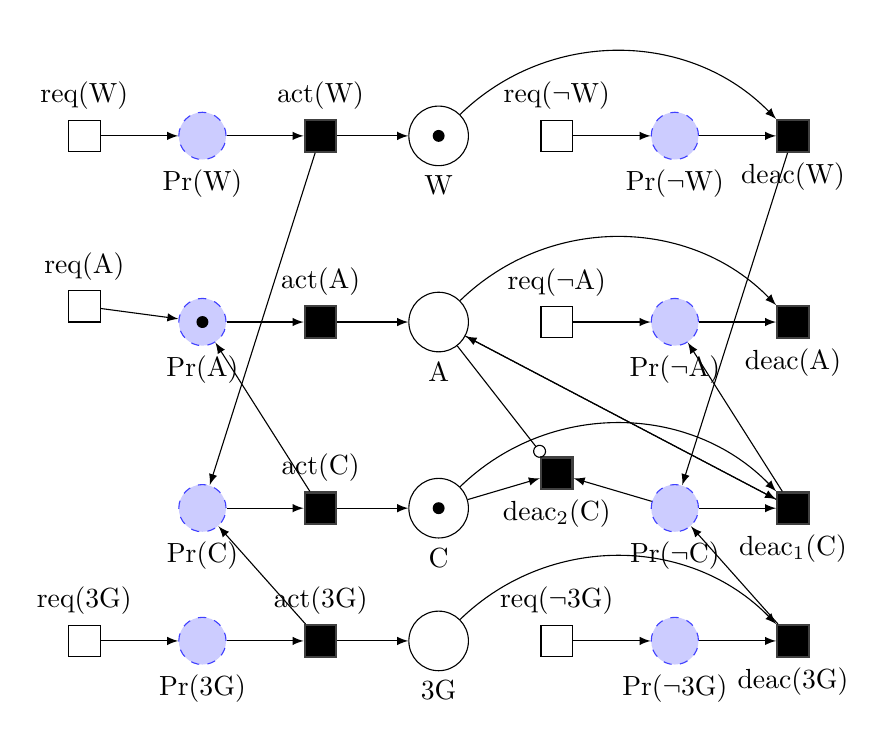
\begin{tikzpicture}[node distance=1.5cm, >=stealth',bend angle=45,auto]
            % WiFi PART

            \node[transition,									label=above:req(W)] (t1) {};
            \node[dplace,right of=t1,tokens=0,label=below:Pr(W)] (p1) {};
            \node[btransition, right of=p1,		label=above:act(W)] (t2) {};
            \node[place, right of=t2,tokens=1,label=below:W] (p2) {};
            \node[transition, right of=p2,		label=above:req($\lnot$W)] (t3) {};
            \node[dplace,right of=t3,tokens=0,label=below:Pr($\lnot$W)] (p3) {};
            \node[btransition, right of=p3,		label=below:deac(W)] (t4) {};

            \path[-latex] (t1) edge node {} (p1);
            \path[-latex] (p1) edge node {} (t2);
            \path[-latex] (t2) edge node {} (p2);
            \path[-latex] (p2) edge[bend left=45] node {} (t4);
            \path[-latex] (t3) edge node {} (p3);
            \path[-latex] (p3) edge node {} (t4);


            % AudioStream PART

            \node[transition,below =1.75cm of t1,  label=above:req(A)] (t13) {};
            \node[dplace, below = 1.75cm of p1,tokens=1, label=below:Pr(A)] (p10) {};
            \node[btransition, right of=p10,    label=above:act(A)] (t14) {};
            \node[place, right of=t14,tokens=0, label=below:A] (p11) {};
            \node[transition, right of=p11,		label=above:req($\lnot$A)] (t15) {};
            \node[dplace, below =1.75cm of p3,     label=below:Pr($\lnot$A)] (p12) {};
            \node[btransition, right of=p12,    label=below:deac(A)] (t16) {};

            \path[-latex] (t13) edge node {} (p10);
            \path[-latex] (p10) edge node {} (t14);
            \path[-latex] (t14) edge node {} (p11);
            \path[-latex] (p11) edge[bend left=45] node {} (t16);
            \path[-latex] (t15) edge node {} (p12);
            \path[-latex] (p12) edge node {} (t16);

            % Connectivity PART

            %\node[transition,below =2cm of t1,	label=above:req(C)] (t9) {};
            \node[dplace, below = 1.75cm of p10,					label=below:Pr(C)] (p7) {};
            \node[btransition, right of=p7,			label=above:act(C)] (t10) {};
            \node[place, right of=t10,tokens=1,	label=below:C] (p8) {};
            %\node[transition, right of=p8,			label=above:req($\lnot$C)] (t11) {};
            \node[dplace, below =1.75cm of p12,					label=below:Pr($\lnot$C)] (p9) {};
            \node[btransition, right of=p9,			label=below:deac$_1$(C)] (t12) {};
            \node[btransition, below=1.5cm of t15,     label=below:deac$_2$(C)] (t17) {};

            %\path[-latex] (t9) edge node {} (p7);
            \path[-latex] (p7) edge node {} (t10);
            \path[-latex] (t10) edge node {} (p8);
            \path[-latex] (p8) edge[bend left=45] node {} (t12);
            %\path[-latex] (t11) edge node {} (p9);
            \path[-latex] (p9) edge node {} (t12);

            % 3G PART

            \node[transition,below =6cm of t1,	label=above:req(3G)] (t5) {};
            \node[dplace, right of=t5,					label=below:Pr(3G)] (p4) {};
            \node[btransition, right of=p4,			label=above:act(3G)] (t6) {};
            \node[place, right of=t6,tokens=0,	label=below:3G] (p5) {};
            \node[transition, right of=p5,			label=above:req($\lnot$3G)] (t7) {};
            \node[dplace, right of=t7,					label=below:Pr($\lnot$3G)] (p6) {};
            \node[btransition, right of=p6,			label=below:deac(3G)] (t8) {};

            \path[-latex] (t5) edge node {} (p4);
            \path[-latex] (p4) edge node {} (t6);
            \path[-latex] (t6) edge node {} (p5);
            \path[-latex] (p5) edge[bend left=45] node {} (t8);
            \path[-latex] (t7) edge node {} (p6);
            \path[-latex] (p6) edge node {} (t8);

            % Connections of Contexts

            \path[-latex] (t2) edge node {} (p7);
            \path[-latex] (t6) edge node {} (p7);
            \path[-latex] (t4) edge node {} (p9);
            \path[-latex] (t8) edge node {} (p9);


            % Connections of Contexts

            \path[-latex] (t10) edge node {} (p10);
            \path[-latex] (t12) edge node {} (p11);
            \path[-latex] (p11) edge node {} (t12);
            \path[-latex] (t12) edge node {} (p12);
            \path[-latex] (p8) edge node {} (t17);
            \path[-latex] (p9) edge node {} (t17);

            \path[-o] (p11) edge node {} (t17);

        \end{tikzpicture}
    \end{figure}
\end{frame}


\begin{frame}[noframenumbering,plain]
    \begin{figure}[!ht]
        \centering
        \scriptsize
        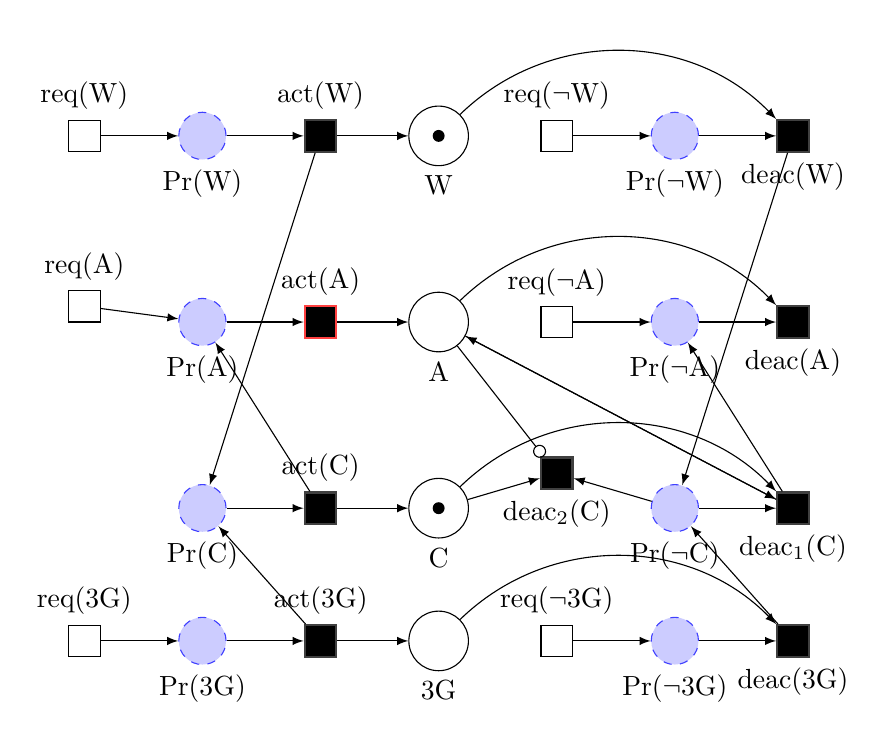
\begin{tikzpicture}[node distance=1.5cm, >=stealth',bend angle=45,auto]
            % WiFi PART

            \node[transition,									label=above:req(W)] (t1) {};
            \node[dplace,right of=t1,tokens=0,label=below:Pr(W)] (p1) {};
            \node[btransition, right of=p1,		label=above:act(W)] (t2) {};
            \node[place, right of=t2,tokens=1,label=below:W] (p2) {};
            \node[transition, right of=p2,		label=above:req($\lnot$W)] (t3) {};
            \node[dplace,right of=t3,tokens=0,label=below:Pr($\lnot$W)] (p3) {};
            \node[btransition, right of=p3,		label=below:deac(W)] (t4) {};

            \path[-latex] (t1) edge node {} (p1);
            \path[-latex] (p1) edge node {} (t2);
            \path[-latex] (t2) edge node {} (p2);
            \path[-latex] (p2) edge[bend left=45] node {} (t4);
            \path[-latex] (t3) edge node {} (p3);
            \path[-latex] (p3) edge node {} (t4);


            % AudioStream PART

            \node[transition,below =1.75cm of t1,  label=above:req(A)] (t13) {};
            \node[dplace, below = 1.75cm of p1,    label=below:Pr(A)] (p10) {};
            \node[rbtransition, right of=p10,    label=above:act(A)] (t14) {};
            \node[place, right of=t14,tokens=0, label=below:A] (p11) {};
            \node[transition, right of=p11,		label=above:req($\lnot$A)] (t15) {};
            \node[dplace, below =1.75cm of p3,     label=below:Pr($\lnot$A)] (p12) {};
            \node[btransition, right of=p12,    label=below:deac(A)] (t16) {};

            \path[-latex] (t13) edge node {} (p10);
            \path[-latex] (p10) edge node {} (t14);
            \path[-latex] (t14) edge node {} (p11);
            \path[-latex] (p11) edge[bend left=45] node {} (t16);
            \path[-latex] (t15) edge node {} (p12);
            \path[-latex] (p12) edge node {} (t16);

            % Connectivity PART

            %\node[transition,below =2cm of t1,	label=above:req(C)] (t9) {};
            \node[dplace, below = 1.75cm of p10,					label=below:Pr(C)] (p7) {};
            \node[btransition, right of=p7,			label=above:act(C)] (t10) {};
            \node[place, right of=t10,tokens=1,	label=below:C] (p8) {};
            %\node[transition, right of=p8,			label=above:req($\lnot$C)] (t11) {};
            \node[dplace, below =1.75cm of p12,					label=below:Pr($\lnot$C)] (p9) {};
            \node[btransition, right of=p9,			label=below:deac$_1$(C)] (t12) {};
            \node[btransition, below=1.5cm of t15,     label=below:deac$_2$(C)] (t17) {};

            %\path[-latex] (t9) edge node {} (p7);
            \path[-latex] (p7) edge node {} (t10);
            \path[-latex] (t10) edge node {} (p8);
            \path[-latex] (p8) edge[bend left=45] node {} (t12);
            %\path[-latex] (t11) edge node {} (p9);
            \path[-latex] (p9) edge node {} (t12);

            % 3G PART

            \node[transition,below =6cm of t1,	label=above:req(3G)] (t5) {};
            \node[dplace, right of=t5,					label=below:Pr(3G)] (p4) {};
            \node[btransition, right of=p4,			label=above:act(3G)] (t6) {};
            \node[place, right of=t6,tokens=0,	label=below:3G] (p5) {};
            \node[transition, right of=p5,			label=above:req($\lnot$3G)] (t7) {};
            \node[dplace, right of=t7,					label=below:Pr($\lnot$3G)] (p6) {};
            \node[btransition, right of=p6,			label=below:deac(3G)] (t8) {};

            \path[-latex] (t5) edge node {} (p4);
            \path[-latex] (p4) edge node {} (t6);
            \path[-latex] (t6) edge node {} (p5);
            \path[-latex] (p5) edge[bend left=45] node {} (t8);
            \path[-latex] (t7) edge node {} (p6);
            \path[-latex] (p6) edge node {} (t8);

            % Connections of Contexts

            \path[-latex] (t2) edge node {} (p7);
            \path[-latex] (t6) edge node {} (p7);
            \path[-latex] (t4) edge node {} (p9);
            \path[-latex] (t8) edge node {} (p9);


            % Connections of Contexts

            \path[-latex] (t10) edge node {} (p10);
            \path[-latex] (t12) edge node {} (p11);
            \path[-latex] (p11) edge node {} (t12);
            \path[-latex] (t12) edge node {} (p12);
            \path[-latex] (p8) edge node {} (t17);
            \path[-latex] (p9) edge node {} (t17);

            \path[-o] (p11) edge node {} (t17);

        \end{tikzpicture}
    \end{figure}
\end{frame}


\begin{frame}[noframenumbering,plain]
    \begin{figure}[!ht]
        \centering
        \scriptsize
        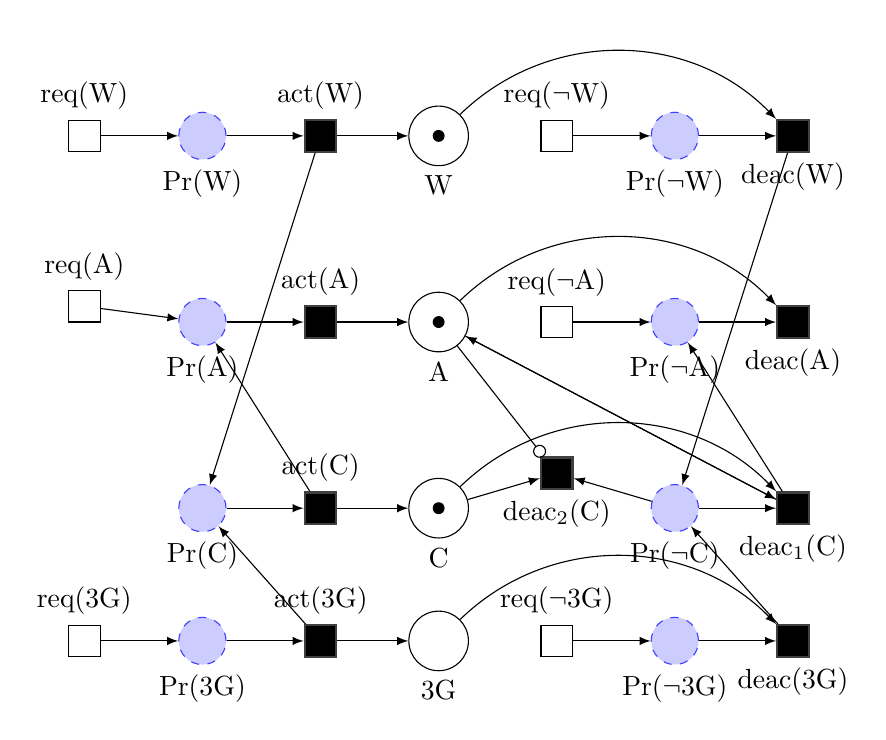
\begin{tikzpicture}[node distance=1.5cm, >=stealth',bend angle=45,auto]
            % WiFi PART

            \node[transition,									label=above:req(W)] (t1) {};
            \node[dplace,right of=t1,tokens=0,label=below:Pr(W)] (p1) {};
            \node[btransition, right of=p1,		label=above:act(W)] (t2) {};
            \node[place, right of=t2,tokens=1,label=below:W] (p2) {};
            \node[transition, right of=p2,		label=above:req($\lnot$W)] (t3) {};
            \node[dplace,right of=t3,tokens=0,label=below:Pr($\lnot$W)] (p3) {};
            \node[btransition, right of=p3,		label=below:deac(W)] (t4) {};

            \path[-latex] (t1) edge node {} (p1);
            \path[-latex] (p1) edge node {} (t2);
            \path[-latex] (t2) edge node {} (p2);
            \path[-latex] (p2) edge[bend left=45] node {} (t4);
            \path[-latex] (t3) edge node {} (p3);
            \path[-latex] (p3) edge node {} (t4);


            % AudioStream PART

            \node[transition,below =1.75cm of t1,  label=above:req(A)] (t13) {};
            \node[dplace, below = 1.75cm of p1,    label=below:Pr(A)] (p10) {};
            \node[btransition, right of=p10,    label=above:act(A)] (t14) {};
            \node[place, right of=t14,tokens=1, label=below:A] (p11) {};
            \node[transition, right of=p11,		label=above:req($\lnot$A)] (t15) {};
            \node[dplace, below =1.75cm of p3,     label=below:Pr($\lnot$A)] (p12) {};
            \node[btransition, right of=p12,    label=below:deac(A)] (t16) {};

            \path[-latex] (t13) edge node {} (p10);
            \path[-latex] (p10) edge node {} (t14);
            \path[-latex] (t14) edge node {} (p11);
            \path[-latex] (p11) edge[bend left=45] node {} (t16);
            \path[-latex] (t15) edge node {} (p12);
            \path[-latex] (p12) edge node {} (t16);

            % Connectivity PART

            %\node[transition,below =2cm of t1,	label=above:req(C)] (t9) {};
            \node[dplace, below = 1.75cm of p10,					label=below:Pr(C)] (p7) {};
            \node[btransition, right of=p7,			label=above:act(C)] (t10) {};
            \node[place, right of=t10,tokens=1,	label=below:C] (p8) {};
            %\node[transition, right of=p8,			label=above:req($\lnot$C)] (t11) {};
            \node[dplace, below =1.75cm of p12,					label=below:Pr($\lnot$C)] (p9) {};
            \node[btransition, right of=p9,			label=below:deac$_1$(C)] (t12) {};
            \node[btransition, below=1.5cm of t15,     label=below:deac$_2$(C)] (t17) {};

            %\path[-latex] (t9) edge node {} (p7);
            \path[-latex] (p7) edge node {} (t10);
            \path[-latex] (t10) edge node {} (p8);
            \path[-latex] (p8) edge[bend left=45] node {} (t12);
            %\path[-latex] (t11) edge node {} (p9);
            \path[-latex] (p9) edge node {} (t12);

            % 3G PART

            \node[transition,below =6cm of t1,	label=above:req(3G)] (t5) {};
            \node[dplace, right of=t5,					label=below:Pr(3G)] (p4) {};
            \node[btransition, right of=p4,			label=above:act(3G)] (t6) {};
            \node[place, right of=t6,tokens=0,	label=below:3G] (p5) {};
            \node[transition, right of=p5,			label=above:req($\lnot$3G)] (t7) {};
            \node[dplace, right of=t7,					label=below:Pr($\lnot$3G)] (p6) {};
            \node[btransition, right of=p6,			label=below:deac(3G)] (t8) {};

            \path[-latex] (t5) edge node {} (p4);
            \path[-latex] (p4) edge node {} (t6);
            \path[-latex] (t6) edge node {} (p5);
            \path[-latex] (p5) edge[bend left=45] node {} (t8);
            \path[-latex] (t7) edge node {} (p6);
            \path[-latex] (p6) edge node {} (t8);

            % Connections of Contexts

            \path[-latex] (t2) edge node {} (p7);
            \path[-latex] (t6) edge node {} (p7);
            \path[-latex] (t4) edge node {} (p9);
            \path[-latex] (t8) edge node {} (p9);


            % Connections of Contexts

            \path[-latex] (t10) edge node {} (p10);
            \path[-latex] (t12) edge node {} (p11);
            \path[-latex] (p11) edge node {} (t12);
            \path[-latex] (t12) edge node {} (p12);
            \path[-latex] (p8) edge node {} (t17);
            \path[-latex] (p9) edge node {} (t17);

            \path[-o] (p11) edge node {} (t17);

        \end{tikzpicture}
    \end{figure}
\end{frame}


\begin{frame}[noframenumbering]
    \frametitle{Relation between contexts}
    \begin{figure}[!ht]
        \centering
        \scriptsize
        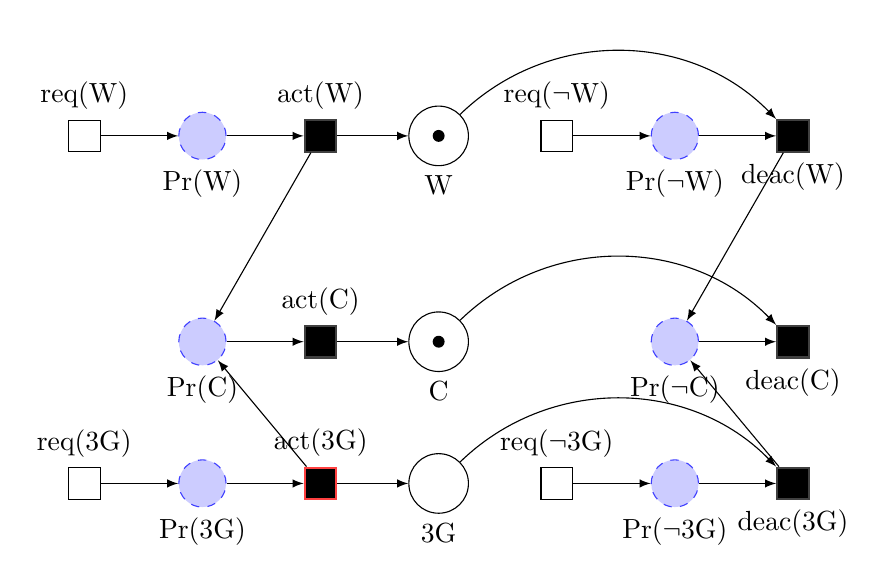
\begin{tikzpicture}[node distance=1.5cm, >=stealth',bend angle=45,auto]
            % WiFi PART

            \node[transition,									label=above:req(W)] (t1) {};
            \node[dplace,right of=t1,tokens=0,label=below:Pr(W)] (p1) {};
            \node[btransition, right of=p1,		label=above:act(W)] (t2) {};
            \node[place, right of=t2,tokens=1,label=below:W] (p2) {};
            \node[transition, right of=p2,		label=above:req($\lnot$W)] (t3) {};
            \node[dplace,right of=t3,tokens=0,label=below:Pr($\lnot$W)] (p3) {};
            \node[btransition, right of=p3,		label=below:deac(W)] (t4) {};

            \path[-latex] (t1) edge node {} (p1);
            \path[-latex] (p1) edge node {} (t2);
            \path[-latex] (t2) edge node {} (p2);
            \path[-latex] (p2) edge[bend left=45] node {} (t4);
            \path[-latex] (t3) edge node {} (p3);
            \path[-latex] (p3) edge node {} (t4);

            % 3G PART

            \node[transition,below =4cm of t1,	label=above:req(3G)] (t5) {};
            \node[dplace, right of=t5,					label=below:Pr(3G)] (p4) {};
            \node[rbtransition, right of=p4,			label=above:act(3G)] (t6) {};
            \node[place, right of=t6,tokens=0,	label=below:3G] (p5) {};
            \node[transition, right of=p5,			label=above:req($\lnot$3G)] (t7) {};
            \node[dplace, right of=t7,					label=below:Pr($\lnot$3G)] (p6) {};
            \node[btransition, right of=p6,			label=below:deac(3G)] (t8) {};

            \path[-latex] (t5) edge node {} (p4);
            \path[-latex] (p4) edge node {} (t6);
            \path[-latex] (t6) edge node {} (p5);
            \path[-latex] (p5) edge[bend left=45] node {} (t8);
            \path[-latex] (t7) edge node {} (p6);
            \path[-latex] (p6) edge node {} (t8);

            % Connectivity PART

            %\node[transition,below =2cm of t1,	label=above:req(C)] (t9) {};
            \node[dplace, below = 2cm of p1,					label=below:Pr(C)] (p7) {};
            \node[btransition, right of=p7,			label=above:act(C)] (t10) {};
            \node[place, right of=t10,tokens=1,	label=below:C] (p8) {};
            %\node[transition, right of=p8,			label=above:req($\lnot$C)] (t11) {};
            \node[dplace, below =2cm of p3,					label=below:Pr($\lnot$C)] (p9) {};
            \node[btransition, right of=p9,			label=below:deac(C)] (t12) {};

            %\path[-latex] (t9) edge node {} (p7);
            \path[-latex] (p7) edge node {} (t10);
            \path[-latex] (t10) edge node {} (p8);
            \path[-latex] (p8) edge[bend left=45] node {} (t12);
            %\path[-latex] (t11) edge node {} (p9);
            \path[-latex] (p9) edge node {} (t12);

            % Connections of Contexts

            \path[-latex] (t2) edge node {} (p7);
            \path[-latex] (t6) edge node {} (p7);
            \path[-latex] (t4) edge node {} (p9);
            \path[-latex] (t8) edge node {} (p9);

        \end{tikzpicture}
    \end{figure}
\end{frame}


\begin{frame}[noframenumbering]
    \frametitle{Relation between contexts}
    \begin{figure}[!ht]
        \centering
        \scriptsize
        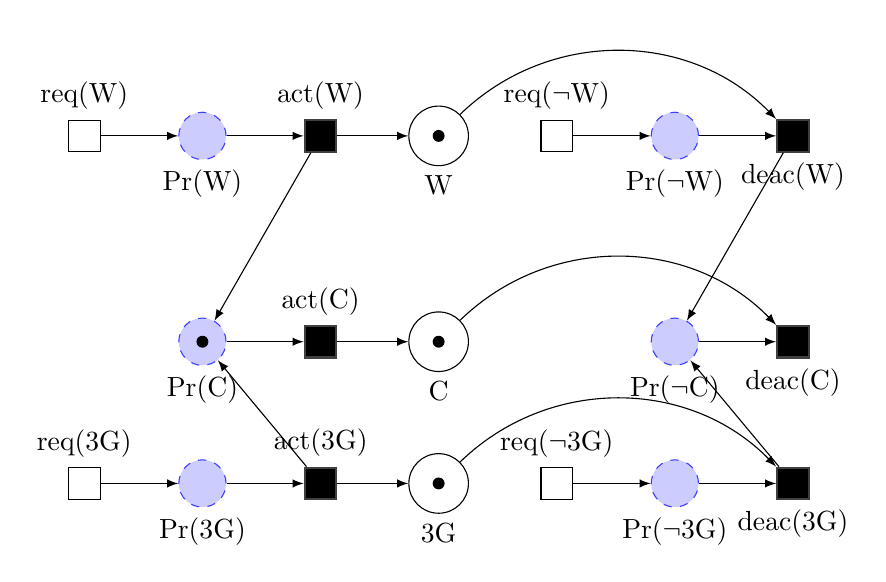
\begin{tikzpicture}[node distance=1.5cm, >=stealth',bend angle=45,auto]
            % WiFi PART

            \node[transition,									label=above:req(W)] (t1) {};
            \node[dplace,right of=t1,tokens=0,label=below:Pr(W)] (p1) {};
            \node[btransition, right of=p1,		label=above:act(W)] (t2) {};
            \node[place, right of=t2,tokens=1,label=below:W] (p2) {};
            \node[transition, right of=p2,		label=above:req($\lnot$W)] (t3) {};
            \node[dplace,right of=t3,tokens=0,label=below:Pr($\lnot$W)] (p3) {};
            \node[btransition, right of=p3,		label=below:deac(W)] (t4) {};

            \path[-latex] (t1) edge node {} (p1);
            \path[-latex] (p1) edge node {} (t2);
            \path[-latex] (t2) edge node {} (p2);
            \path[-latex] (p2) edge[bend left=45] node {} (t4);
            \path[-latex] (t3) edge node {} (p3);
            \path[-latex] (p3) edge node {} (t4);

            % 3G PART

            \node[transition,below =4cm of t1,	label=above:req(3G)] (t5) {};
            \node[dplace, right of=t5,					label=below:Pr(3G)] (p4) {};
            \node[btransition, right of=p4,			label=above:act(3G)] (t6) {};
            \node[place, right of=t6,tokens=1,	label=below:3G] (p5) {};
            \node[transition, right of=p5,			label=above:req($\lnot$3G)] (t7) {};
            \node[dplace, right of=t7,					label=below:Pr($\lnot$3G)] (p6) {};
            \node[btransition, right of=p6,			label=below:deac(3G)] (t8) {};

            \path[-latex] (t5) edge node {} (p4);
            \path[-latex] (p4) edge node {} (t6);
            \path[-latex] (t6) edge node {} (p5);
            \path[-latex] (p5) edge[bend left=45] node {} (t8);
            \path[-latex] (t7) edge node {} (p6);
            \path[-latex] (p6) edge node {} (t8);

            % Connectivity PART

            %\node[transition,below =2cm of t1,	label=above:req(C)] (t9) {};
            \node[dplace,below=2cm of p1,tokens=1,label=below:Pr(C)] (p7) {};
            \node[btransition, right of=p7,			label=above:act(C)] (t10) {};
            \node[place, right of=t10,tokens=1,	label=below:C] (p8) {};
            %\node[transition, right of=p8,			label=above:req($\lnot$C)] (t11) {};
            \node[dplace, below =2cm of p3,					label=below:Pr($\lnot$C)] (p9) {};
            \node[btransition, right of=p9,			label=below:deac(C)] (t12) {};

            %\path[-latex] (t9) edge node {} (p7);
            \path[-latex] (p7) edge node {} (t10);
            \path[-latex] (t10) edge node {} (p8);
            \path[-latex] (p8) edge[bend left=45] node {} (t12);
            %\path[-latex] (t11) edge node {} (p9);
            \path[-latex] (p9) edge node {} (t12);

            % Connections of Contexts

            \path[-latex] (t2) edge node {} (p7);
            \path[-latex] (t6) edge node {} (p7);
            \path[-latex] (t4) edge node {} (p9);
            \path[-latex] (t8) edge node {} (p9);

        \end{tikzpicture}
    \end{figure}
\end{frame}


\begin{frame}[noframenumbering,plain]
    \begin{figure}[!ht]
        \centering
        \scriptsize
        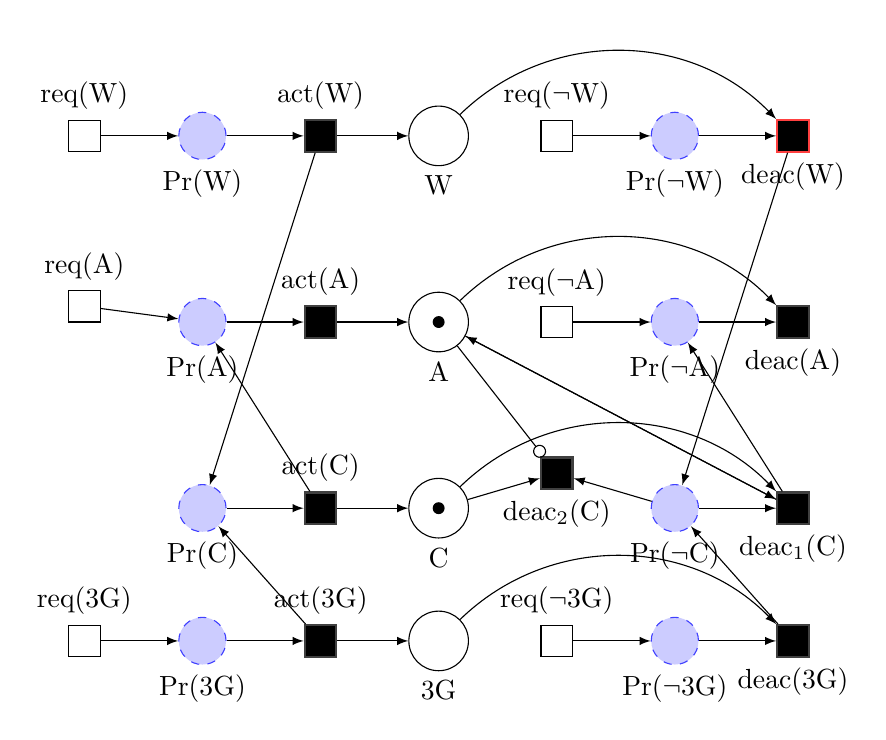
\begin{tikzpicture}[node distance=1.5cm, >=stealth',bend angle=45,auto]
            % WiFi PART

            \node[transition,									label=above:req(W)] (t1) {};
            \node[dplace,right of=t1,tokens=0,label=below:Pr(W)] (p1) {};
            \node[btransition, right of=p1,		label=above:act(W)] (t2) {};
            \node[place, right of=t2,tokens=0,label=below:W] (p2) {};
            \node[transition, right of=p2,		label=above:req($\lnot$W)] (t3) {};
            \node[dplace,right of=t3,tokens=0,label=below:Pr($\lnot$W)] (p3) {};
            \node[rbtransition, right of=p3,		label=below:deac(W)] (t4) {};

            \path[-latex] (t1) edge node {} (p1);
            \path[-latex] (p1) edge node {} (t2);
            \path[-latex] (t2) edge node {} (p2);
            \path[-latex] (p2) edge[bend left=45] node {} (t4);
            \path[-latex] (t3) edge node {} (p3);
            \path[-latex] (p3) edge node {} (t4);


            % AudioStream PART

            \node[transition,below =1.75cm of t1,  label=above:req(A)] (t13) {};
            \node[dplace, below = 1.75cm of p1,    label=below:Pr(A)] (p10) {};
            \node[btransition, right of=p10,    label=above:act(A)] (t14) {};
            \node[place, right of=t14,tokens=1, label=below:A] (p11) {};
            \node[transition, right of=p11,		label=above:req($\lnot$A)] (t15) {};
            \node[dplace, below =1.75cm of p3,     label=below:Pr($\lnot$A)] (p12) {};
            \node[btransition, right of=p12,    label=below:deac(A)] (t16) {};

            \path[-latex] (t13) edge node {} (p10);
            \path[-latex] (p10) edge node {} (t14);
            \path[-latex] (t14) edge node {} (p11);
            \path[-latex] (p11) edge[bend left=45] node {} (t16);
            \path[-latex] (t15) edge node {} (p12);
            \path[-latex] (p12) edge node {} (t16);

            % Connectivity PART

            %\node[transition,below =2cm of t1,	label=above:req(C)] (t9) {};
            \node[dplace, below = 1.75cm of p10,					label=below:Pr(C)] (p7) {};
            \node[btransition, right of=p7,			label=above:act(C)] (t10) {};
            \node[place, right of=t10,tokens=1,	label=below:C] (p8) {};
            %\node[transition, right of=p8,			label=above:req($\lnot$C)] (t11) {};
            \node[dplace, below =1.75cm of p12,					label=below:Pr($\lnot$C)] (p9) {};
            \node[btransition, right of=p9,			label=below:deac$_1$(C)] (t12) {};
            \node[btransition, below=1.5cm of t15,     label=below:deac$_2$(C)] (t17) {};

            %\path[-latex] (t9) edge node {} (p7);
            \path[-latex] (p7) edge node {} (t10);
            \path[-latex] (t10) edge node {} (p8);
            \path[-latex] (p8) edge[bend left=45] node {} (t12);
            %\path[-latex] (t11) edge node {} (p9);
            \path[-latex] (p9) edge node {} (t12);

            % 3G PART

            \node[transition,below =6cm of t1,	label=above:req(3G)] (t5) {};
            \node[dplace, right of=t5,					label=below:Pr(3G)] (p4) {};
            \node[btransition, right of=p4,			label=above:act(3G)] (t6) {};
            \node[place, right of=t6,tokens=0,	label=below:3G] (p5) {};
            \node[transition, right of=p5,			label=above:req($\lnot$3G)] (t7) {};
            \node[dplace, right of=t7,					label=below:Pr($\lnot$3G)] (p6) {};
            \node[btransition, right of=p6,			label=below:deac(3G)] (t8) {};

            \path[-latex] (t5) edge node {} (p4);
            \path[-latex] (p4) edge node {} (t6);
            \path[-latex] (t6) edge node {} (p5);
            \path[-latex] (p5) edge[bend left=45] node {} (t8);
            \path[-latex] (t7) edge node {} (p6);
            \path[-latex] (p6) edge node {} (t8);

            % Connections of Contexts

            \path[-latex] (t2) edge node {} (p7);
            \path[-latex] (t6) edge node {} (p7);
            \path[-latex] (t4) edge node {} (p9);
            \path[-latex] (t8) edge node {} (p9);


            % Connections of Contexts

            \path[-latex] (t10) edge node {} (p10);
            \path[-latex] (t12) edge node {} (p11);
            \path[-latex] (p11) edge node {} (t12);
            \path[-latex] (t12) edge node {} (p12);
            \path[-latex] (p8) edge node {} (t17);
            \path[-latex] (p9) edge node {} (t17);

            \path[-o] (p11) edge node {} (t17);

        \end{tikzpicture}
    \end{figure}
\end{frame}


\begin{frame}[noframenumbering,plain]
    \begin{figure}[!ht]
        \centering
        \scriptsize
        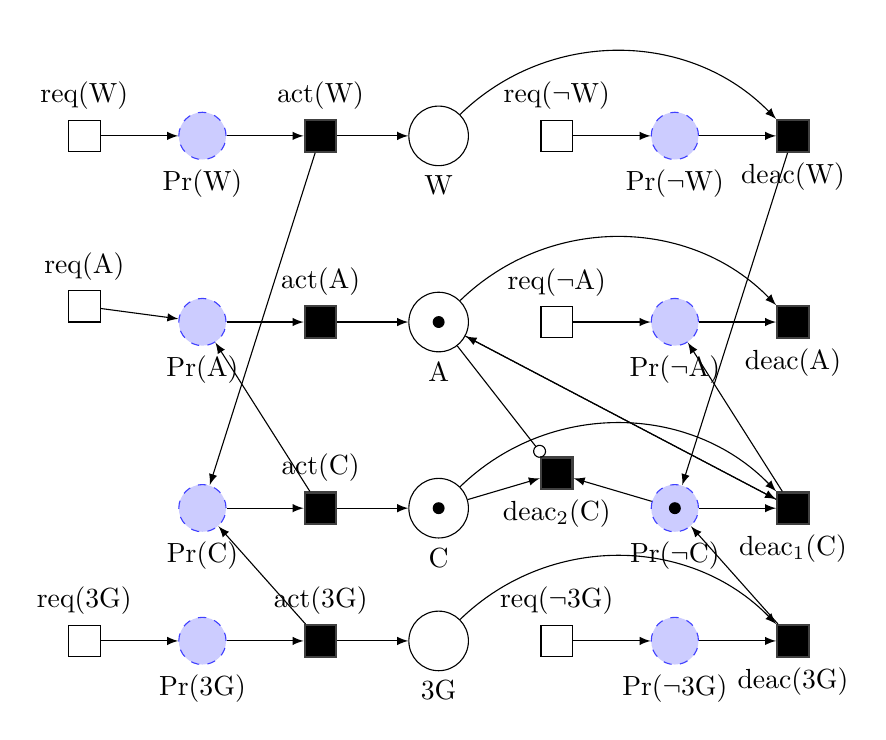
\begin{tikzpicture}[node distance=1.5cm, >=stealth',bend angle=45,auto]
            % WiFi PART

            \node[transition,									label=above:req(W)] (t1) {};
            \node[dplace,right of=t1,tokens=0,label=below:Pr(W)] (p1) {};
            \node[btransition, right of=p1,		label=above:act(W)] (t2) {};
            \node[place, right of=t2,tokens=0,label=below:W] (p2) {};
            \node[transition, right of=p2,		label=above:req($\lnot$W)] (t3) {};
            \node[dplace,right of=t3,tokens=0,label=below:Pr($\lnot$W)] (p3) {};
            \node[btransition, right of=p3,		label=below:deac(W)] (t4) {};

            \path[-latex] (t1) edge node {} (p1);
            \path[-latex] (p1) edge node {} (t2);
            \path[-latex] (t2) edge node {} (p2);
            \path[-latex] (p2) edge[bend left=45] node {} (t4);
            \path[-latex] (t3) edge node {} (p3);
            \path[-latex] (p3) edge node {} (t4);


            % AudioStream PART

            \node[transition,below =1.75cm of t1,  label=above:req(A)] (t13) {};
            \node[dplace, below = 1.75cm of p1,    label=below:Pr(A)] (p10) {};
            \node[btransition, right of=p10,    label=above:act(A)] (t14) {};
            \node[place, right of=t14,tokens=1, label=below:A] (p11) {};
            \node[transition, right of=p11,		label=above:req($\lnot$A)] (t15) {};
            \node[dplace, below =1.75cm of p3,     label=below:Pr($\lnot$A)] (p12) {};
            \node[btransition, right of=p12,    label=below:deac(A)] (t16) {};

            \path[-latex] (t13) edge node {} (p10);
            \path[-latex] (p10) edge node {} (t14);
            \path[-latex] (t14) edge node {} (p11);
            \path[-latex] (p11) edge[bend left=45] node {} (t16);
            \path[-latex] (t15) edge node {} (p12);
            \path[-latex] (p12) edge node {} (t16);

            % Connectivity PART

            %\node[transition,below =2cm of t1,	label=above:req(C)] (t9) {};
            \node[dplace, below = 1.75cm of p10,					label=below:Pr(C)] (p7) {};
            \node[btransition, right of=p7,			label=above:act(C)] (t10) {};
            \node[place, right of=t10,tokens=1,	label=below:C] (p8) {};
            %\node[transition, right of=p8,			label=above:req($\lnot$C)] (t11) {};
            \node[dplace, below =1.75cm of p12,tokens=1,				label=below:Pr($\lnot$C)] (p9) {};
            \node[btransition, right of=p9,			label=below:deac$_1$(C)] (t12) {};
            \node[btransition, below=1.5cm of t15,     label=below:deac$_2$(C)] (t17) {};

            %\path[-latex] (t9) edge node {} (p7);
            \path[-latex] (p7) edge node {} (t10);
            \path[-latex] (t10) edge node {} (p8);
            \path[-latex] (p8) edge[bend left=45] node {} (t12);
            %\path[-latex] (t11) edge node {} (p9);
            \path[-latex] (p9) edge node {} (t12);

            % 3G PART

            \node[transition,below =6cm of t1,	label=above:req(3G)] (t5) {};
            \node[dplace, right of=t5,					label=below:Pr(3G)] (p4) {};
            \node[btransition, right of=p4,			label=above:act(3G)] (t6) {};
            \node[place, right of=t6,tokens=0,	label=below:3G] (p5) {};
            \node[transition, right of=p5,			label=above:req($\lnot$3G)] (t7) {};
            \node[dplace, right of=t7,					label=below:Pr($\lnot$3G)] (p6) {};
            \node[btransition, right of=p6,			label=below:deac(3G)] (t8) {};

            \path[-latex] (t5) edge node {} (p4);
            \path[-latex] (p4) edge node {} (t6);
            \path[-latex] (t6) edge node {} (p5);
            \path[-latex] (p5) edge[bend left=45] node {} (t8);
            \path[-latex] (t7) edge node {} (p6);
            \path[-latex] (p6) edge node {} (t8);

            % Connections of Contexts

            \path[-latex] (t2) edge node {} (p7);
            \path[-latex] (t6) edge node {} (p7);
            \path[-latex] (t4) edge node {} (p9);
            \path[-latex] (t8) edge node {} (p9);


            % Connections of Contexts

            \path[-latex] (t10) edge node {} (p10);
            \path[-latex] (t12) edge node {} (p11);
            \path[-latex] (p11) edge node {} (t12);
            \path[-latex] (t12) edge node {} (p12);
            \path[-latex] (p8) edge node {} (t17);
            \path[-latex] (p9) edge node {} (t17);

            \path[-o] (p11) edge node {} (t17);

        \end{tikzpicture}
    \end{figure}
\end{frame}


\begin{frame}[noframenumbering]
    \frametitle{Relation between contexts}
    \begin{figure}[!ht]
        \centering
        \scriptsize
        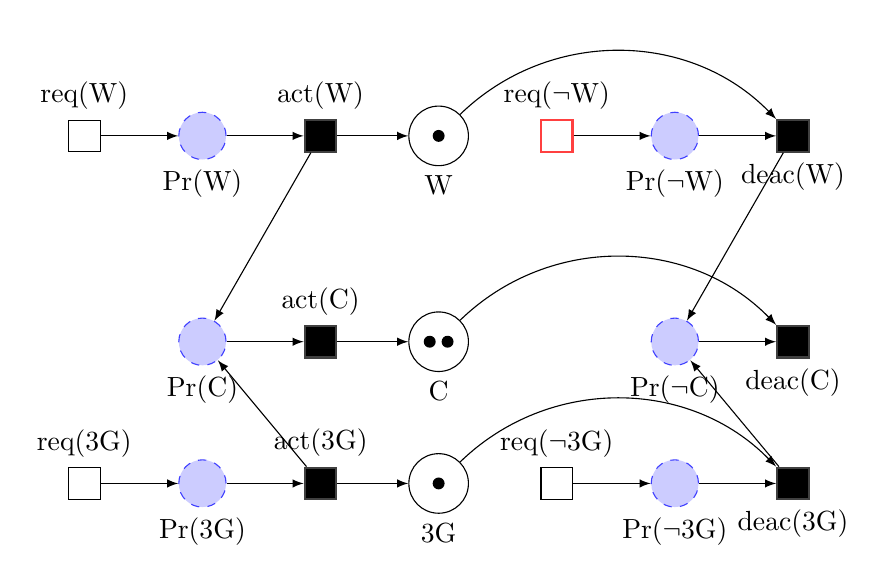
\begin{tikzpicture}[node distance=1.5cm, >=stealth',bend angle=45,auto]
            % WiFi PART

            \node[transition,									label=above:req(W)] (t1) {};
            \node[dplace,right of=t1,tokens=0,label=below:Pr(W)] (p1) {};
            \node[btransition, right of=p1,		label=above:act(W)] (t2) {};
            \node[place, right of=t2,tokens=1,label=below:W] (p2) {};
            \node[rtransition, right of=p2,		label=above:req($\lnot$W)] (t3) {};
            \node[dplace,right of=t3,tokens=0,label=below:Pr($\lnot$W)] (p3) {};
            \node[btransition, right of=p3,		label=below:deac(W)] (t4) {};

            \path[-latex] (t1) edge node {} (p1);
            \path[-latex] (p1) edge node {} (t2);
            \path[-latex] (t2) edge node {} (p2);
            \path[-latex] (p2) edge[bend left=45] node {} (t4);
            \path[-latex] (t3) edge node {} (p3);
            \path[-latex] (p3) edge node {} (t4);

            % 3G PART

            \node[transition,below =4cm of t1,	label=above:req(3G)] (t5) {};
            \node[dplace, right of=t5,					label=below:Pr(3G)] (p4) {};
            \node[btransition, right of=p4,			label=above:act(3G)] (t6) {};
            \node[place, right of=t6,tokens=1,	label=below:3G] (p5) {};
            \node[transition, right of=p5,			label=above:req($\lnot$3G)] (t7) {};
            \node[dplace, right of=t7,					label=below:Pr($\lnot$3G)] (p6) {};
            \node[btransition, right of=p6,			label=below:deac(3G)] (t8) {};

            \path[-latex] (t5) edge node {} (p4);
            \path[-latex] (p4) edge node {} (t6);
            \path[-latex] (t6) edge node {} (p5);
            \path[-latex] (p5) edge[bend left=45] node {} (t8);
            \path[-latex] (t7) edge node {} (p6);
            \path[-latex] (p6) edge node {} (t8);

            % Connectivity PART

            %\node[transition,below =2cm of t1,	label=above:req(C)] (t9) {};
            \node[dplace, below = 2cm of p1,					label=below:Pr(C)] (p7) {};
            \node[btransition, right of=p7,			label=above:act(C)] (t10) {};
            \node[place, right of=t10,tokens=2,	label=below:C] (p8) {};
            %\node[transition, right of=p8,			label=above:req($\lnot$C)] (t11) {};
            \node[dplace, below =2cm of p3,					label=below:Pr($\lnot$C)] (p9) {};
            \node[btransition, right of=p9,			label=below:deac(C)] (t12) {};

            %\path[-latex] (t9) edge node {} (p7);
            \path[-latex] (p7) edge node {} (t10);
            \path[-latex] (t10) edge node {} (p8);
            \path[-latex] (p8) edge[bend left=45] node {} (t12);
            %\path[-latex] (t11) edge node {} (p9);
            \path[-latex] (p9) edge node {} (t12);

            % Connections of Contexts

            \path[-latex] (t2) edge node {} (p7);
            \path[-latex] (t6) edge node {} (p7);
            \path[-latex] (t4) edge node {} (p9);
            \path[-latex] (t8) edge node {} (p9);

        \end{tikzpicture}
    \end{figure}
\end{frame}


\begin{frame}[noframenumbering,plain]
    \begin{figure}[!ht]
        \centering
        \scriptsize
        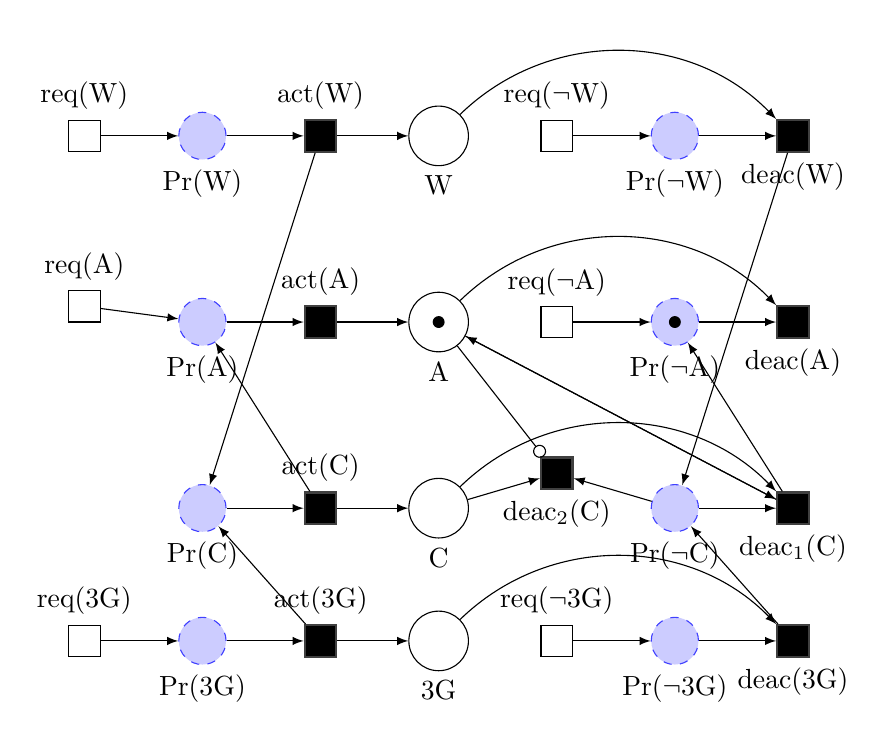
\begin{tikzpicture}[node distance=1.5cm, >=stealth',bend angle=45,auto]
            % WiFi PART

            \node[transition,									label=above:req(W)] (t1) {};
            \node[dplace,right of=t1,tokens=0,label=below:Pr(W)] (p1) {};
            \node[btransition, right of=p1,		label=above:act(W)] (t2) {};
            \node[place, right of=t2,tokens=0,label=below:W] (p2) {};
            \node[transition, right of=p2,		label=above:req($\lnot$W)] (t3) {};
            \node[dplace,right of=t3,tokens=0,label=below:Pr($\lnot$W)] (p3) {};
            \node[btransition, right of=p3,		label=below:deac(W)] (t4) {};

            \path[-latex] (t1) edge node {} (p1);
            \path[-latex] (p1) edge node {} (t2);
            \path[-latex] (t2) edge node {} (p2);
            \path[-latex] (p2) edge[bend left=45] node {} (t4);
            \path[-latex] (t3) edge node {} (p3);
            \path[-latex] (p3) edge node {} (t4);


            % AudioStream PART

            \node[transition,below =1.75cm of t1,  label=above:req(A)] (t13) {};
            \node[dplace, below = 1.75cm of p1,    label=below:Pr(A)] (p10) {};
            \node[btransition, right of=p10,    label=above:act(A)] (t14) {};
            \node[place, right of=t14,tokens=1, label=below:A] (p11) {};
            \node[transition, right of=p11,		label=above:req($\lnot$A)] (t15) {};
            \node[dplace, below =1.75cm of p3,tokens=1,     label=below:Pr($\lnot$A)] (p12) {};
            \node[btransition, right of=p12,    label=below:deac(A)] (t16) {};

            \path[-latex] (t13) edge node {} (p10);
            \path[-latex] (p10) edge node {} (t14);
            \path[-latex] (t14) edge node {} (p11);
            \path[-latex] (p11) edge[bend left=45] node {} (t16);
            \path[-latex] (t15) edge node {} (p12);
            \path[-latex] (p12) edge node {} (t16);

            % Connectivity PART

            %\node[transition,below =2cm of t1,	label=above:req(C)] (t9) {};
            \node[dplace, below = 1.75cm of p10,					label=below:Pr(C)] (p7) {};
            \node[btransition, right of=p7,			label=above:act(C)] (t10) {};
            \node[place, right of=t10,tokens=0,	label=below:C] (p8) {};
            %\node[transition, right of=p8,			label=above:req($\lnot$C)] (t11) {};
            \node[dplace, below =1.75cm of p12,					label=below:Pr($\lnot$C)] (p9) {};
            \node[btransition, right of=p9,			label=below:deac$_1$(C)] (t12) {};
            \node[btransition, below=1.5cm of t15,     label=below:deac$_2$(C)] (t17) {};

            %\path[-latex] (t9) edge node {} (p7);
            \path[-latex] (p7) edge node {} (t10);
            \path[-latex] (t10) edge node {} (p8);
            \path[-latex] (p8) edge[bend left=45] node {} (t12);
            %\path[-latex] (t11) edge node {} (p9);
            \path[-latex] (p9) edge node {} (t12);

            % 3G PART

            \node[transition,below =6cm of t1,	label=above:req(3G)] (t5) {};
            \node[dplace, right of=t5,					label=below:Pr(3G)] (p4) {};
            \node[btransition, right of=p4,			label=above:act(3G)] (t6) {};
            \node[place, right of=t6,tokens=0,	label=below:3G] (p5) {};
            \node[transition, right of=p5,			label=above:req($\lnot$3G)] (t7) {};
            \node[dplace, right of=t7,					label=below:Pr($\lnot$3G)] (p6) {};
            \node[btransition, right of=p6,			label=below:deac(3G)] (t8) {};

            \path[-latex] (t5) edge node {} (p4);
            \path[-latex] (p4) edge node {} (t6);
            \path[-latex] (t6) edge node {} (p5);
            \path[-latex] (p5) edge[bend left=45] node {} (t8);
            \path[-latex] (t7) edge node {} (p6);
            \path[-latex] (p6) edge node {} (t8);

            % Connections of Contexts

            \path[-latex] (t2) edge node {} (p7);
            \path[-latex] (t6) edge node {} (p7);
            \path[-latex] (t4) edge node {} (p9);
            \path[-latex] (t8) edge node {} (p9);


            % Connections of Contexts

            \path[-latex] (t10) edge node {} (p10);
            \path[-latex] (t12) edge node {} (p11);
            \path[-latex] (p11) edge node {} (t12);
            \path[-latex] (t12) edge node {} (p12);
            \path[-latex] (p8) edge node {} (t17);
            \path[-latex] (p9) edge node {} (t17);

            \path[-o] (p11) edge node {} (t17);

        \end{tikzpicture}
    \end{figure}
\end{frame}


\begin{frame}[noframenumbering,plain]
    \begin{figure}[!ht]
        \centering
        \scriptsize
        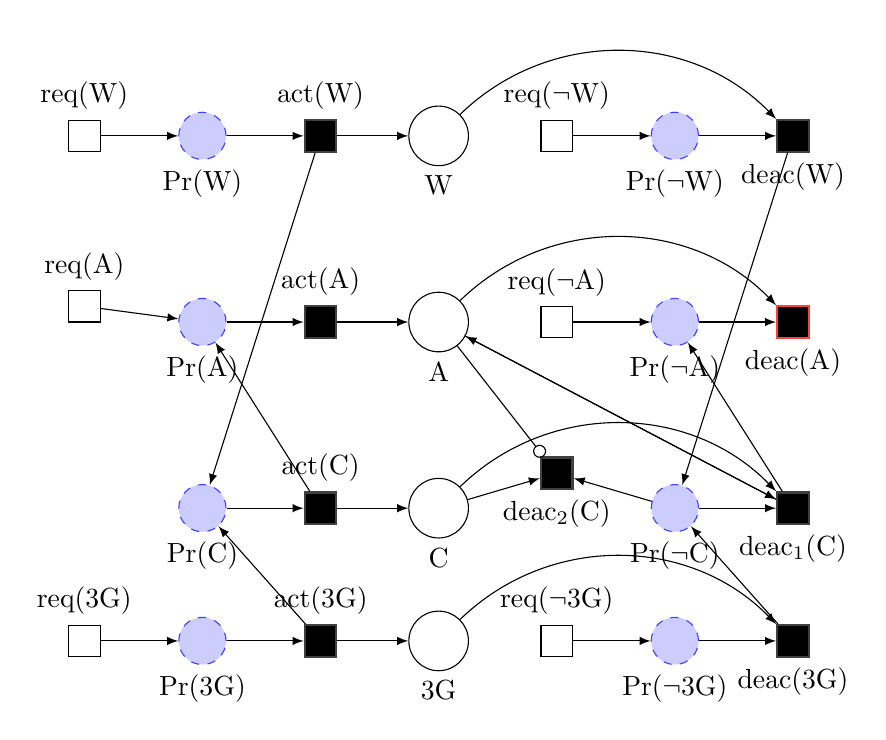
\begin{tikzpicture}[node distance=1.5cm, >=stealth',bend angle=45,auto]
            % WiFi PART

            \node[transition,									label=above:req(W)] (t1) {};
            \node[dplace,right of=t1,tokens=0,label=below:Pr(W)] (p1) {};
            \node[btransition, right of=p1,		label=above:act(W)] (t2) {};
            \node[place, right of=t2,tokens=0,label=below:W] (p2) {};
            \node[transition, right of=p2,		label=above:req($\lnot$W)] (t3) {};
            \node[dplace,right of=t3,tokens=0,label=below:Pr($\lnot$W)] (p3) {};
            \node[btransition, right of=p3,		label=below:deac(W)] (t4) {};

            \path[-latex] (t1) edge node {} (p1);
            \path[-latex] (p1) edge node {} (t2);
            \path[-latex] (t2) edge node {} (p2);
            \path[-latex] (p2) edge[bend left=45] node {} (t4);
            \path[-latex] (t3) edge node {} (p3);
            \path[-latex] (p3) edge node {} (t4);


            % AudioStream PART

            \node[transition,below =1.75cm of t1,  label=above:req(A)] (t13) {};
            \node[dplace, below = 1.75cm of p1,    label=below:Pr(A)] (p10) {};
            \node[btransition, right of=p10,    label=above:act(A)] (t14) {};
            \node[place, right of=t14,tokens=0, label=below:A] (p11) {};
            \node[transition, right of=p11,		label=above:req($\lnot$A)] (t15) {};
            \node[dplace, below =1.75cm of p3,     label=below:Pr($\lnot$A)] (p12) {};
            \node[rbtransition, right of=p12,    label=below:deac(A)] (t16) {};

            \path[-latex] (t13) edge node {} (p10);
            \path[-latex] (p10) edge node {} (t14);
            \path[-latex] (t14) edge node {} (p11);
            \path[-latex] (p11) edge[bend left=45] node {} (t16);
            \path[-latex] (t15) edge node {} (p12);
            \path[-latex] (p12) edge node {} (t16);

            % Connectivity PART

            %\node[transition,below =2cm of t1,	label=above:req(C)] (t9) {};
            \node[dplace, below = 1.75cm of p10,					label=below:Pr(C)] (p7) {};
            \node[btransition, right of=p7,			label=above:act(C)] (t10) {};
            \node[place, right of=t10,tokens=0,	label=below:C] (p8) {};
            %\node[transition, right of=p8,			label=above:req($\lnot$C)] (t11) {};
            \node[dplace, below =1.75cm of p12,					label=below:Pr($\lnot$C)] (p9) {};
            \node[btransition, right of=p9,			label=below:deac$_1$(C)] (t12) {};
            \node[btransition, below=1.5cm of t15,     label=below:deac$_2$(C)] (t17) {};

            %\path[-latex] (t9) edge node {} (p7);
            \path[-latex] (p7) edge node {} (t10);
            \path[-latex] (t10) edge node {} (p8);
            \path[-latex] (p8) edge[bend left=45] node {} (t12);
            %\path[-latex] (t11) edge node {} (p9);
            \path[-latex] (p9) edge node {} (t12);

            % 3G PART

            \node[transition,below =6cm of t1,	label=above:req(3G)] (t5) {};
            \node[dplace, right of=t5,					label=below:Pr(3G)] (p4) {};
            \node[btransition, right of=p4,			label=above:act(3G)] (t6) {};
            \node[place, right of=t6,tokens=0,	label=below:3G] (p5) {};
            \node[transition, right of=p5,			label=above:req($\lnot$3G)] (t7) {};
            \node[dplace, right of=t7,					label=below:Pr($\lnot$3G)] (p6) {};
            \node[btransition, right of=p6,			label=below:deac(3G)] (t8) {};

            \path[-latex] (t5) edge node {} (p4);
            \path[-latex] (p4) edge node {} (t6);
            \path[-latex] (t6) edge node {} (p5);
            \path[-latex] (p5) edge[bend left=45] node {} (t8);
            \path[-latex] (t7) edge node {} (p6);
            \path[-latex] (p6) edge node {} (t8);

            % Connections of Contexts

            \path[-latex] (t2) edge node {} (p7);
            \path[-latex] (t6) edge node {} (p7);
            \path[-latex] (t4) edge node {} (p9);
            \path[-latex] (t8) edge node {} (p9);


            % Connections of Contexts

            \path[-latex] (t10) edge node {} (p10);
            \path[-latex] (t12) edge node {} (p11);
            \path[-latex] (p11) edge node {} (t12);
            \path[-latex] (t12) edge node {} (p12);
            \path[-latex] (p8) edge node {} (t17);
            \path[-latex] (p9) edge node {} (t17);

            \path[-o] (p11) edge node {} (t17);

        \end{tikzpicture}
    \end{figure}
\end{frame}


\begin{frame}[noframenumbering]
    \frametitle{Relation between contexts}
    \begin{figure}[!ht]
        \centering
        \scriptsize
        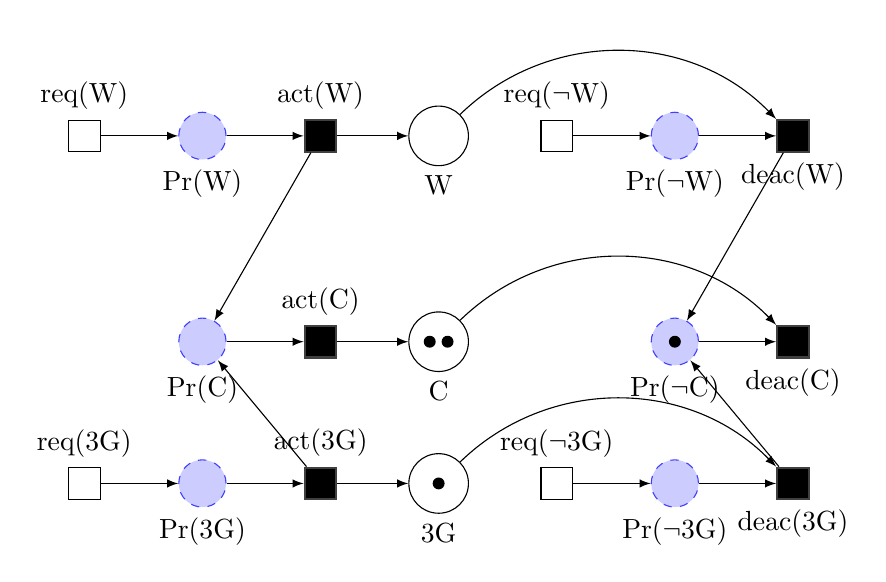
\begin{tikzpicture}[node distance=1.5cm, >=stealth',bend angle=45,auto]
            % WiFi PART

            \node[transition,									label=above:req(W)] (t1) {};
            \node[dplace,right of=t1,tokens=0,label=below:Pr(W)] (p1) {};
            \node[btransition, right of=p1,		label=above:act(W)] (t2) {};
            \node[place, right of=t2,tokens=0,label=below:W] (p2) {};
            \node[transition, right of=p2,		label=above:req($\lnot$W)] (t3) {};
            \node[dplace,right of=t3,tokens=0,label=below:Pr($\lnot$W)] (p3) {};
            \node[btransition, right of=p3,		label=below:deac(W)] (t4) {};

            \path[-latex] (t1) edge node {} (p1);
            \path[-latex] (p1) edge node {} (t2);
            \path[-latex] (t2) edge node {} (p2);
            \path[-latex] (p2) edge[bend left=45] node {} (t4);
            \path[-latex] (t3) edge node {} (p3);
            \path[-latex] (p3) edge node {} (t4);

            % 3G PART

            \node[transition,below =4cm of t1,	label=above:req(3G)] (t5) {};
            \node[dplace, right of=t5,					label=below:Pr(3G)] (p4) {};
            \node[btransition, right of=p4,			label=above:act(3G)] (t6) {};
            \node[place, right of=t6,tokens=1,	label=below:3G] (p5) {};
            \node[transition, right of=p5,			label=above:req($\lnot$3G)] (t7) {};
            \node[dplace, right of=t7,					label=below:Pr($\lnot$3G)] (p6) {};
            \node[btransition, right of=p6,			label=below:deac(3G)] (t8) {};

            \path[-latex] (t5) edge node {} (p4);
            \path[-latex] (p4) edge node {} (t6);
            \path[-latex] (t6) edge node {} (p5);
            \path[-latex] (p5) edge[bend left=45] node {} (t8);
            \path[-latex] (t7) edge node {} (p6);
            \path[-latex] (p6) edge node {} (t8);

            % Connectivity PART

            %\node[transition,below =2cm of t1,	label=above:req(C)] (t9) {};
            \node[dplace, below = 2cm of p1,					label=below:Pr(C)] (p7) {};
            \node[btransition, right of=p7,			label=above:act(C)] (t10) {};
            \node[place, right of=t10,tokens=2,	label=below:C] (p8) {};
            %\node[transition, right of=p8,			label=above:req($\lnot$C)] (t11) {};
            \node[dplace,below=2cm of p3,tokens=1,label=below:Pr($\lnot$C)] (p9) {};
            \node[btransition, right of=p9,			label=below:deac(C)] (t12) {};

            %\path[-latex] (t9) edge node {} (p7);
            \path[-latex] (p7) edge node {} (t10);
            \path[-latex] (t10) edge node {} (p8);
            \path[-latex] (p8) edge[bend left=45] node {} (t12);
            %\path[-latex] (t11) edge node {} (p9);
            \path[-latex] (p9) edge node {} (t12);

            % Connections of Contexts

            \path[-latex] (t2) edge node {} (p7);
            \path[-latex] (t6) edge node {} (p7);
            \path[-latex] (t4) edge node {} (p9);
            \path[-latex] (t8) edge node {} (p9);

        \end{tikzpicture}
    \end{figure}
\end{frame}


\begin{frame}[noframenumbering]
    \frametitle{Relation between contexts}
    \begin{figure}[!ht]
        \centering
        \scriptsize
        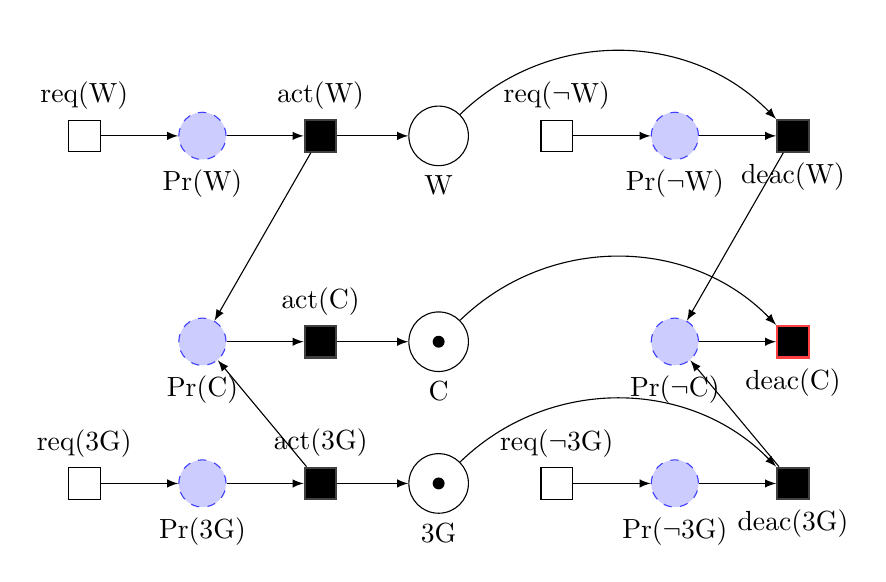
\begin{tikzpicture}[node distance=1.5cm, >=stealth',bend angle=45,auto]
            % WiFi PART

            \node[transition,									label=above:req(W)] (t1) {};
            \node[dplace,right of=t1,tokens=0,label=below:Pr(W)] (p1) {};
            \node[btransition, right of=p1,		label=above:act(W)] (t2) {};
            \node[place, right of=t2,tokens=0,label=below:W] (p2) {};
            \node[transition, right of=p2,		label=above:req($\lnot$W)] (t3) {};
            \node[dplace,right of=t3,tokens=0,label=below:Pr($\lnot$W)] (p3) {};
            \node[btransition, right of=p3,		label=below:deac(W)] (t4) {};

            \path[-latex] (t1) edge node {} (p1);
            \path[-latex] (p1) edge node {} (t2);
            \path[-latex] (t2) edge node {} (p2);
            \path[-latex] (p2) edge[bend left=45] node {} (t4);
            \path[-latex] (t3) edge node {} (p3);
            \path[-latex] (p3) edge node {} (t4);

            % 3G PART

            \node[transition,below =4cm of t1,	label=above:req(3G)] (t5) {};
            \node[dplace, right of=t5,					label=below:Pr(3G)] (p4) {};
            \node[btransition, right of=p4,			label=above:act(3G)] (t6) {};
            \node[place, right of=t6,tokens=1,	label=below:3G] (p5) {};
            \node[transition, right of=p5,			label=above:req($\lnot$3G)] (t7) {};
            \node[dplace, right of=t7,					label=below:Pr($\lnot$3G)] (p6) {};
            \node[btransition, right of=p6,			label=below:deac(3G)] (t8) {};

            \path[-latex] (t5) edge node {} (p4);
            \path[-latex] (p4) edge node {} (t6);
            \path[-latex] (t6) edge node {} (p5);
            \path[-latex] (p5) edge[bend left=45] node {} (t8);
            \path[-latex] (t7) edge node {} (p6);
            \path[-latex] (p6) edge node {} (t8);

            % Connectivity PART

            %\node[transition,below =2cm of t1,	label=above:req(C)] (t9) {};
            \node[dplace, below = 2cm of p1,					label=below:Pr(C)] (p7) {};
            \node[btransition, right of=p7,			label=above:act(C)] (t10) {};
            \node[place, right of=t10,tokens=1,	label=below:C] (p8) {};
            %\node[transition, right of=p8,			label=above:req($\lnot$C)] (t11) {};
            \node[dplace, below =2cm of p3,					label=below:Pr($\lnot$C)] (p9) {};
            \node[rbtransition, right of=p9,			label=below:deac(C)] (t12) {};

            %\path[-latex] (t9) edge node {} (p7);
            \path[-latex] (p7) edge node {} (t10);
            \path[-latex] (t10) edge node {} (p8);
            \path[-latex] (p8) edge[bend left=45] node {} (t12);
            %\path[-latex] (t11) edge node {} (p9);
            \path[-latex] (p9) edge node {} (t12);

            % Connections of Contexts

            \path[-latex] (t2) edge node {} (p7);
            \path[-latex] (t6) edge node {} (p7);
            \path[-latex] (t4) edge node {} (p9);
            \path[-latex] (t8) edge node {} (p9);

        \end{tikzpicture}
    \end{figure}
\end{frame}


\begin{frame}[noframenumbering]
    \frametitle{Relation between contexts}
    \begin{figure}[!ht]
        \centering
        \scriptsize
        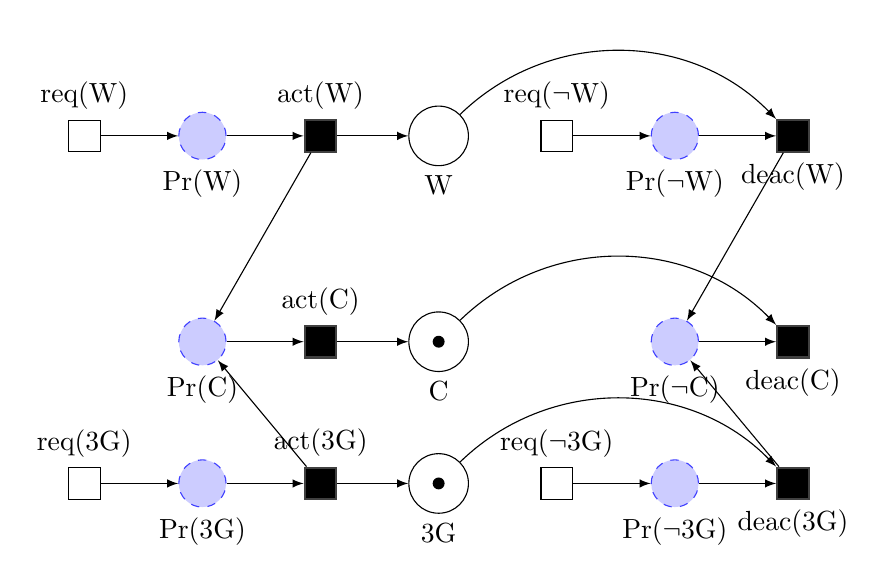
\begin{tikzpicture}[node distance=1.5cm, >=stealth',bend angle=45,auto]
            % WiFi PART

            \node[transition,									label=above:req(W)] (t1) {};
            \node[dplace,right of=t1,tokens=0,label=below:Pr(W)] (p1) {};
            \node[btransition, right of=p1,		label=above:act(W)] (t2) {};
            \node[place, right of=t2,tokens=0,label=below:W] (p2) {};
            \node[transition, right of=p2,		label=above:req($\lnot$W)] (t3) {};
            \node[dplace,right of=t3,tokens=0,label=below:Pr($\lnot$W)] (p3) {};
            \node[btransition, right of=p3,		label=below:deac(W)] (t4) {};

            \path[-latex] (t1) edge node {} (p1);
            \path[-latex] (p1) edge node {} (t2);
            \path[-latex] (t2) edge node {} (p2);
            \path[-latex] (p2) edge[bend left=45] node {} (t4);
            \path[-latex] (t3) edge node {} (p3);
            \path[-latex] (p3) edge node {} (t4);

            % 3G PART

            \node[transition,below =4cm of t1,	label=above:req(3G)] (t5) {};
            \node[dplace, right of=t5,					label=below:Pr(3G)] (p4) {};
            \node[btransition, right of=p4,			label=above:act(3G)] (t6) {};
            \node[place, right of=t6,tokens=1,	label=below:3G] (p5) {};
            \node[transition, right of=p5,			label=above:req($\lnot$3G)] (t7) {};
            \node[dplace, right of=t7,					label=below:Pr($\lnot$3G)] (p6) {};
            \node[btransition, right of=p6,			label=below:deac(3G)] (t8) {};

            \path[-latex] (t5) edge node {} (p4);
            \path[-latex] (p4) edge node {} (t6);
            \path[-latex] (t6) edge node {} (p5);
            \path[-latex] (p5) edge[bend left=45] node {} (t8);
            \path[-latex] (t7) edge node {} (p6);
            \path[-latex] (p6) edge node {} (t8);

            % Connectivity PART

            %\node[transition,below =2cm of t1,	label=above:req(C)] (t9) {};
            \node[dplace, below = 2cm of p1,					label=below:Pr(C)] (p7) {};
            \node[btransition, right of=p7,			label=above:act(C)] (t10) {};
            \node[place, right of=t10,tokens=1,	label=below:C] (p8) {};
            %\node[transition, right of=p8,			label=above:req($\lnot$C)] (t11) {};
            \node[dplace, below =2cm of p3,					label=below:Pr($\lnot$C)] (p9) {};
            \node[btransition, right of=p9,			label=below:deac(C)] (t12) {};

            %\path[-latex] (t9) edge node {} (p7);
            \path[-latex] (p7) edge node {} (t10);
            \path[-latex] (t10) edge node {} (p8);
            \path[-latex] (p8) edge[bend left=45] node {} (t12);
            %\path[-latex] (t11) edge node {} (p9);
            \path[-latex] (p9) edge node {} (t12);

            % Connections of Contexts

            \path[-latex] (t2) edge node {} (p7);
            \path[-latex] (t6) edge node {} (p7);
            \path[-latex] (t4) edge node {} (p9);
            \path[-latex] (t8) edge node {} (p9);

        \end{tikzpicture}
    \end{figure}
\end{frame}


\begin{frame}
	\frametitle{Causality between contexts}

	\begin{alertblock}{Bad news}
		The relations between contexts are sometimes more complex\ldots
	\end{alertblock}
	\bigskip


	\textbf{Connectivity} activates an \textbf{AudioStream}
	context which will be deactivated as soon as \textbf{Connectivity} becomes inactive.
	\bigskip

	\begin{exampleblock}{Relation type}
		This is called a \textit{causality dependency relation}.
	\end{exampleblock}

	We add a constraint on transitions:

	\begin{figure}[!ht]
		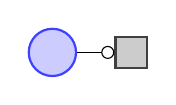
\begin{tikzpicture}
			\tikzstyle{place}=[circle,thick,draw=blue!75,fill=blue!20,minimum size=6mm]
			\tikzstyle{transition}=[rectangle,thick,draw=black!75,
					fill=black!20,minimum size=4mm]

			\node[place] (p1) {};
			\node[transition, right of=p1] (t1) {};

			\path[-o] (p1) edge node {} (t1);
		\end{tikzpicture}
	\end{figure}

	\begin{center}
		\enquote{The transition cannot be fired if there is token(s) in the place}
	\end{center}
\end{frame}

\begin{frame}[plain]
    \begin{figure}[!ht]
        \centering
        \scriptsize
        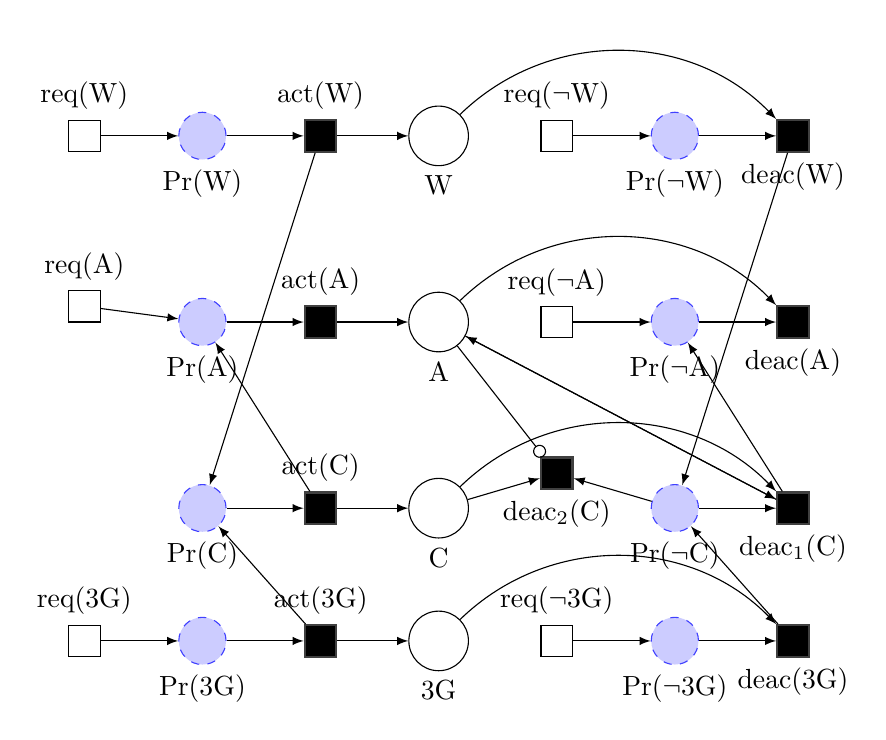
\begin{tikzpicture}[node distance=1.5cm, >=stealth',bend angle=45,auto]
            % WiFi PART

            \node[transition,									label=above:req(W)] (t1) {};
            \node[dplace,right of=t1,tokens=0,label=below:Pr(W)] (p1) {};
            \node[btransition, right of=p1,		label=above:act(W)] (t2) {};
            \node[place, right of=t2,tokens=0,label=below:W] (p2) {};
            \node[transition, right of=p2,		label=above:req($\lnot$W)] (t3) {};
            \node[dplace,right of=t3,tokens=0,label=below:Pr($\lnot$W)] (p3) {};
            \node[btransition, right of=p3,		label=below:deac(W)] (t4) {};

            \path[-latex] (t1) edge node {} (p1);
            \path[-latex] (p1) edge node {} (t2);
            \path[-latex] (t2) edge node {} (p2);
            \path[-latex] (p2) edge[bend left=45] node {} (t4);
            \path[-latex] (t3) edge node {} (p3);
            \path[-latex] (p3) edge node {} (t4);


            % AudioStream PART

            \node[transition,below =1.75cm of t1,  label=above:req(A)] (t13) {};
            \node[dplace, below = 1.75cm of p1,    label=below:Pr(A)] (p10) {};
            \node[btransition, right of=p10,    label=above:act(A)] (t14) {};
            \node[place, right of=t14,tokens=0, label=below:A] (p11) {};
            \node[transition, right of=p11,		label=above:req($\lnot$A)] (t15) {};
            \node[dplace, below =1.75cm of p3,     label=below:Pr($\lnot$A)] (p12) {};
            \node[btransition, right of=p12,    label=below:deac(A)] (t16) {};

            \path[-latex] (t13) edge node {} (p10);
            \path[-latex] (p10) edge node {} (t14);
            \path[-latex] (t14) edge node {} (p11);
            \path[-latex] (p11) edge[bend left=45] node {} (t16);
            \path[-latex] (t15) edge node {} (p12);
            \path[-latex] (p12) edge node {} (t16);

            % Connectivity PART

            %\node[transition,below =2cm of t1,	label=above:req(C)] (t9) {};
            \node[dplace, below = 1.75cm of p10,					label=below:Pr(C)] (p7) {};
            \node[btransition, right of=p7,			label=above:act(C)] (t10) {};
            \node[place, right of=t10,tokens=0,	label=below:C] (p8) {};
            %\node[transition, right of=p8,			label=above:req($\lnot$C)] (t11) {};
            \node[dplace, below =1.75cm of p12,					label=below:Pr($\lnot$C)] (p9) {};
            \node[btransition, right of=p9,			label=below:deac$_1$(C)] (t12) {};
            \node[btransition, below=1.5cm of t15,     label=below:deac$_2$(C)] (t17) {};

            %\path[-latex] (t9) edge node {} (p7);
            \path[-latex] (p7) edge node {} (t10);
            \path[-latex] (t10) edge node {} (p8);
            \path[-latex] (p8) edge[bend left=45] node {} (t12);
            %\path[-latex] (t11) edge node {} (p9);
            \path[-latex] (p9) edge node {} (t12);

            % 3G PART

            \node[transition,below =6cm of t1,	label=above:req(3G)] (t5) {};
            \node[dplace, right of=t5,					label=below:Pr(3G)] (p4) {};
            \node[btransition, right of=p4,			label=above:act(3G)] (t6) {};
            \node[place, right of=t6,tokens=0,	label=below:3G] (p5) {};
            \node[transition, right of=p5,			label=above:req($\lnot$3G)] (t7) {};
            \node[dplace, right of=t7,					label=below:Pr($\lnot$3G)] (p6) {};
            \node[btransition, right of=p6,			label=below:deac(3G)] (t8) {};

            \path[-latex] (t5) edge node {} (p4);
            \path[-latex] (p4) edge node {} (t6);
            \path[-latex] (t6) edge node {} (p5);
            \path[-latex] (p5) edge[bend left=45] node {} (t8);
            \path[-latex] (t7) edge node {} (p6);
            \path[-latex] (p6) edge node {} (t8);

            % Connections of Contexts

            \path[-latex] (t2) edge node {} (p7);
            \path[-latex] (t6) edge node {} (p7);
            \path[-latex] (t4) edge node {} (p9);
            \path[-latex] (t8) edge node {} (p9);


            % Connections of Contexts

            \path[-latex] (t10) edge node {} (p10);
            \path[-latex] (t12) edge node {} (p11);
            \path[-latex] (p11) edge node {} (t12);
            \path[-latex] (t12) edge node {} (p12);
            \path[-latex] (p8) edge node {} (t17);
            \path[-latex] (p9) edge node {} (t17);

            \path[-o] (p11) edge node {} (t17);

        \end{tikzpicture}
    \end{figure}
\end{frame}


\begin{frame}[noframenumbering,plain]
    \begin{figure}[!ht]
        \centering
        \scriptsize
        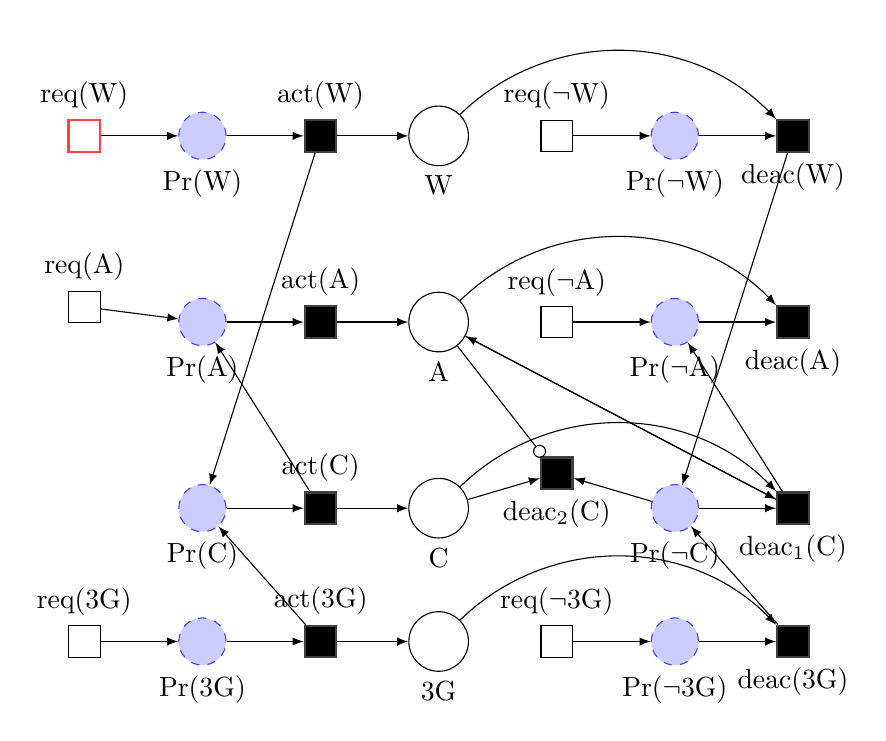
\begin{tikzpicture}[node distance=1.5cm, >=stealth',bend angle=45,auto]
            % WiFi PART

            \node[rtransition,									label=above:req(W)] (t1) {};
            \node[dplace,right of=t1,tokens=0,label=below:Pr(W)] (p1) {};
            \node[btransition, right of=p1,		label=above:act(W)] (t2) {};
            \node[place, right of=t2,tokens=0,label=below:W] (p2) {};
            \node[transition, right of=p2,		label=above:req($\lnot$W)] (t3) {};
            \node[dplace,right of=t3,tokens=0,label=below:Pr($\lnot$W)] (p3) {};
            \node[btransition, right of=p3,		label=below:deac(W)] (t4) {};

            \path[-latex] (t1) edge node {} (p1);
            \path[-latex] (p1) edge node {} (t2);
            \path[-latex] (t2) edge node {} (p2);
            \path[-latex] (p2) edge[bend left=45] node {} (t4);
            \path[-latex] (t3) edge node {} (p3);
            \path[-latex] (p3) edge node {} (t4);


            % AudioStream PART

            \node[transition,below =1.75cm of t1,  label=above:req(A)] (t13) {};
            \node[dplace, below = 1.75cm of p1,    label=below:Pr(A)] (p10) {};
            \node[btransition, right of=p10,    label=above:act(A)] (t14) {};
            \node[place, right of=t14,tokens=0, label=below:A] (p11) {};
            \node[transition, right of=p11,		label=above:req($\lnot$A)] (t15) {};
            \node[dplace, below =1.75cm of p3,     label=below:Pr($\lnot$A)] (p12) {};
            \node[btransition, right of=p12,    label=below:deac(A)] (t16) {};

            \path[-latex] (t13) edge node {} (p10);
            \path[-latex] (p10) edge node {} (t14);
            \path[-latex] (t14) edge node {} (p11);
            \path[-latex] (p11) edge[bend left=45] node {} (t16);
            \path[-latex] (t15) edge node {} (p12);
            \path[-latex] (p12) edge node {} (t16);

            % Connectivity PART

            %\node[transition,below =2cm of t1,	label=above:req(C)] (t9) {};
            \node[dplace, below = 1.75cm of p10,					label=below:Pr(C)] (p7) {};
            \node[btransition, right of=p7,			label=above:act(C)] (t10) {};
            \node[place, right of=t10,tokens=0,	label=below:C] (p8) {};
            %\node[transition, right of=p8,			label=above:req($\lnot$C)] (t11) {};
            \node[dplace, below =1.75cm of p12,					label=below:Pr($\lnot$C)] (p9) {};
            \node[btransition, right of=p9,			label=below:deac$_1$(C)] (t12) {};
            \node[btransition, below=1.5cm of t15,     label=below:deac$_2$(C)] (t17) {};

            %\path[-latex] (t9) edge node {} (p7);
            \path[-latex] (p7) edge node {} (t10);
            \path[-latex] (t10) edge node {} (p8);
            \path[-latex] (p8) edge[bend left=45] node {} (t12);
            %\path[-latex] (t11) edge node {} (p9);
            \path[-latex] (p9) edge node {} (t12);

            % 3G PART

            \node[transition,below =6cm of t1,	label=above:req(3G)] (t5) {};
            \node[dplace, right of=t5,					label=below:Pr(3G)] (p4) {};
            \node[btransition, right of=p4,			label=above:act(3G)] (t6) {};
            \node[place, right of=t6,tokens=0,	label=below:3G] (p5) {};
            \node[transition, right of=p5,			label=above:req($\lnot$3G)] (t7) {};
            \node[dplace, right of=t7,					label=below:Pr($\lnot$3G)] (p6) {};
            \node[btransition, right of=p6,			label=below:deac(3G)] (t8) {};

            \path[-latex] (t5) edge node {} (p4);
            \path[-latex] (p4) edge node {} (t6);
            \path[-latex] (t6) edge node {} (p5);
            \path[-latex] (p5) edge[bend left=45] node {} (t8);
            \path[-latex] (t7) edge node {} (p6);
            \path[-latex] (p6) edge node {} (t8);

            % Connections of Contexts

            \path[-latex] (t2) edge node {} (p7);
            \path[-latex] (t6) edge node {} (p7);
            \path[-latex] (t4) edge node {} (p9);
            \path[-latex] (t8) edge node {} (p9);


            % Connections of Contexts

            \path[-latex] (t10) edge node {} (p10);
            \path[-latex] (t12) edge node {} (p11);
            \path[-latex] (p11) edge node {} (t12);
            \path[-latex] (t12) edge node {} (p12);
            \path[-latex] (p8) edge node {} (t17);
            \path[-latex] (p9) edge node {} (t17);

            \path[-o] (p11) edge node {} (t17);

        \end{tikzpicture}
    \end{figure}
\end{frame}


\begin{frame}[noframenumbering,plain]
    \begin{figure}[!ht]
        \centering
        \scriptsize
        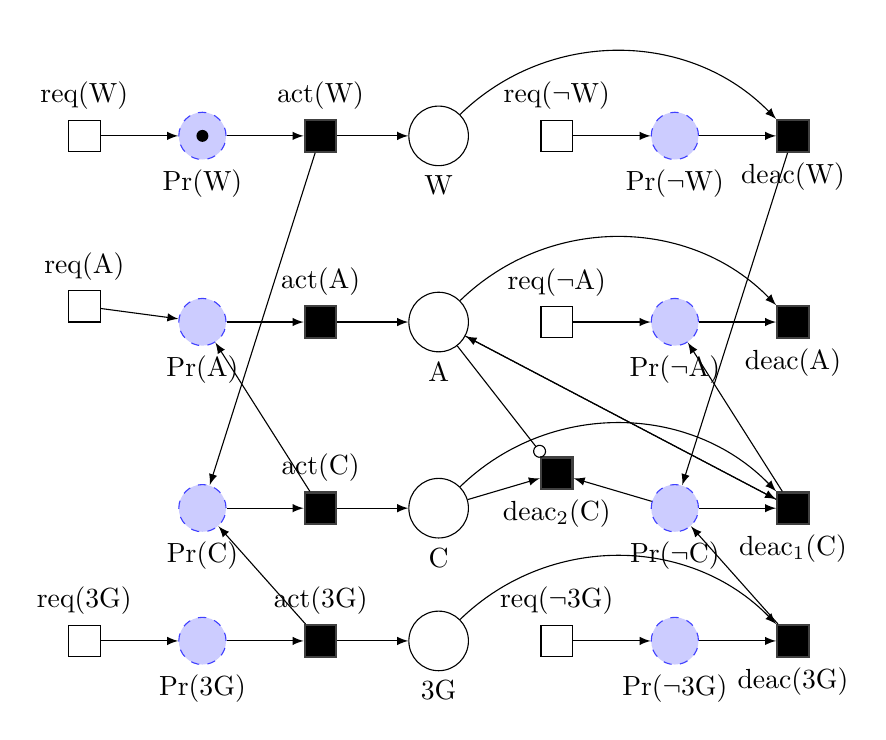
\begin{tikzpicture}[node distance=1.5cm, >=stealth',bend angle=45,auto]
            % WiFi PART

            \node[transition,									label=above:req(W)] (t1) {};
            \node[dplace,right of=t1,tokens=1,label=below:Pr(W)] (p1) {};
            \node[btransition, right of=p1,		label=above:act(W)] (t2) {};
            \node[place, right of=t2,tokens=0,label=below:W] (p2) {};
            \node[transition, right of=p2,		label=above:req($\lnot$W)] (t3) {};
            \node[dplace,right of=t3,tokens=0,label=below:Pr($\lnot$W)] (p3) {};
            \node[btransition, right of=p3,		label=below:deac(W)] (t4) {};

            \path[-latex] (t1) edge node {} (p1);
            \path[-latex] (p1) edge node {} (t2);
            \path[-latex] (t2) edge node {} (p2);
            \path[-latex] (p2) edge[bend left=45] node {} (t4);
            \path[-latex] (t3) edge node {} (p3);
            \path[-latex] (p3) edge node {} (t4);


            % AudioStream PART

            \node[transition,below =1.75cm of t1,  label=above:req(A)] (t13) {};
            \node[dplace, below = 1.75cm of p1,    label=below:Pr(A)] (p10) {};
            \node[btransition, right of=p10,    label=above:act(A)] (t14) {};
            \node[place, right of=t14,tokens=0, label=below:A] (p11) {};
            \node[transition, right of=p11,		label=above:req($\lnot$A)] (t15) {};
            \node[dplace, below =1.75cm of p3,     label=below:Pr($\lnot$A)] (p12) {};
            \node[btransition, right of=p12,    label=below:deac(A)] (t16) {};

            \path[-latex] (t13) edge node {} (p10);
            \path[-latex] (p10) edge node {} (t14);
            \path[-latex] (t14) edge node {} (p11);
            \path[-latex] (p11) edge[bend left=45] node {} (t16);
            \path[-latex] (t15) edge node {} (p12);
            \path[-latex] (p12) edge node {} (t16);

            % Connectivity PART

            %\node[transition,below =2cm of t1,	label=above:req(C)] (t9) {};
            \node[dplace, below = 1.75cm of p10,					label=below:Pr(C)] (p7) {};
            \node[btransition, right of=p7,			label=above:act(C)] (t10) {};
            \node[place, right of=t10,tokens=0,	label=below:C] (p8) {};
            %\node[transition, right of=p8,			label=above:req($\lnot$C)] (t11) {};
            \node[dplace, below =1.75cm of p12,					label=below:Pr($\lnot$C)] (p9) {};
            \node[btransition, right of=p9,			label=below:deac$_1$(C)] (t12) {};
            \node[btransition, below=1.5cm of t15,     label=below:deac$_2$(C)] (t17) {};

            %\path[-latex] (t9) edge node {} (p7);
            \path[-latex] (p7) edge node {} (t10);
            \path[-latex] (t10) edge node {} (p8);
            \path[-latex] (p8) edge[bend left=45] node {} (t12);
            %\path[-latex] (t11) edge node {} (p9);
            \path[-latex] (p9) edge node {} (t12);

            % 3G PART

            \node[transition,below =6cm of t1,	label=above:req(3G)] (t5) {};
            \node[dplace, right of=t5,					label=below:Pr(3G)] (p4) {};
            \node[btransition, right of=p4,			label=above:act(3G)] (t6) {};
            \node[place, right of=t6,tokens=0,	label=below:3G] (p5) {};
            \node[transition, right of=p5,			label=above:req($\lnot$3G)] (t7) {};
            \node[dplace, right of=t7,					label=below:Pr($\lnot$3G)] (p6) {};
            \node[btransition, right of=p6,			label=below:deac(3G)] (t8) {};

            \path[-latex] (t5) edge node {} (p4);
            \path[-latex] (p4) edge node {} (t6);
            \path[-latex] (t6) edge node {} (p5);
            \path[-latex] (p5) edge[bend left=45] node {} (t8);
            \path[-latex] (t7) edge node {} (p6);
            \path[-latex] (p6) edge node {} (t8);

            % Connections of Contexts

            \path[-latex] (t2) edge node {} (p7);
            \path[-latex] (t6) edge node {} (p7);
            \path[-latex] (t4) edge node {} (p9);
            \path[-latex] (t8) edge node {} (p9);


            % Connections of Contexts

            \path[-latex] (t10) edge node {} (p10);
            \path[-latex] (t12) edge node {} (p11);
            \path[-latex] (p11) edge node {} (t12);
            \path[-latex] (t12) edge node {} (p12);
            \path[-latex] (p8) edge node {} (t17);
            \path[-latex] (p9) edge node {} (t17);

            \path[-o] (p11) edge node {} (t17);

        \end{tikzpicture}
    \end{figure}
\end{frame}


\begin{frame}[noframenumbering,plain]
    \begin{figure}[!ht]
        \centering
        \scriptsize
        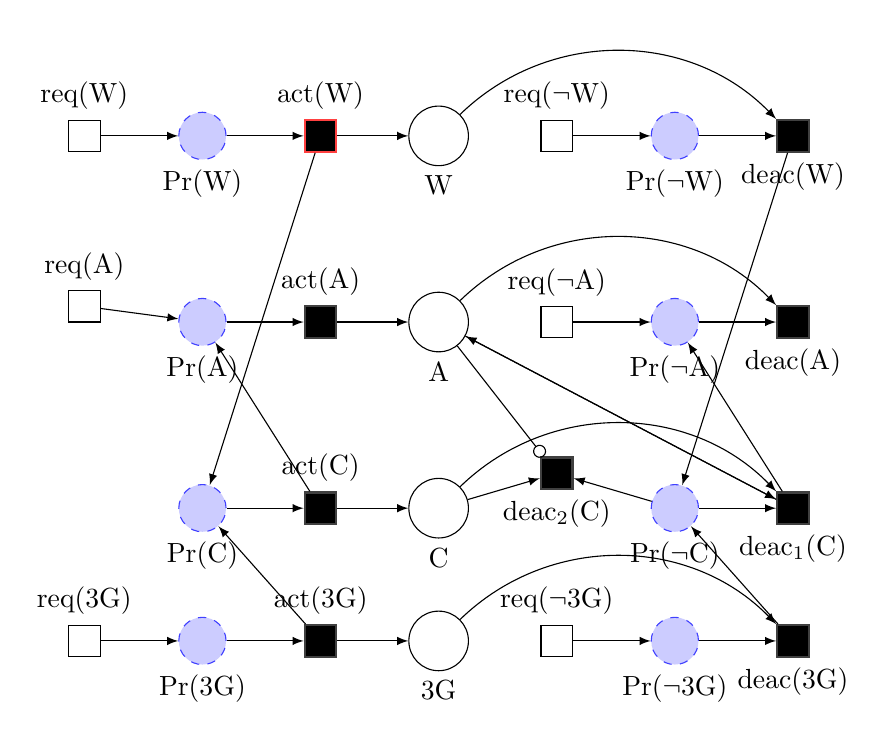
\begin{tikzpicture}[node distance=1.5cm, >=stealth',bend angle=45,auto]
            % WiFi PART

            \node[transition,									label=above:req(W)] (t1) {};
            \node[dplace,right of=t1,tokens=0,label=below:Pr(W)] (p1) {};
            \node[rbtransition, right of=p1,		label=above:act(W)] (t2) {};
            \node[place, right of=t2,tokens=0,label=below:W] (p2) {};
            \node[transition, right of=p2,		label=above:req($\lnot$W)] (t3) {};
            \node[dplace,right of=t3,tokens=0,label=below:Pr($\lnot$W)] (p3) {};
            \node[btransition, right of=p3,		label=below:deac(W)] (t4) {};

            \path[-latex] (t1) edge node {} (p1);
            \path[-latex] (p1) edge node {} (t2);
            \path[-latex] (t2) edge node {} (p2);
            \path[-latex] (p2) edge[bend left=45] node {} (t4);
            \path[-latex] (t3) edge node {} (p3);
            \path[-latex] (p3) edge node {} (t4);


            % AudioStream PART

            \node[transition,below =1.75cm of t1,  label=above:req(A)] (t13) {};
            \node[dplace, below = 1.75cm of p1,    label=below:Pr(A)] (p10) {};
            \node[btransition, right of=p10,    label=above:act(A)] (t14) {};
            \node[place, right of=t14,tokens=0, label=below:A] (p11) {};
            \node[transition, right of=p11,		label=above:req($\lnot$A)] (t15) {};
            \node[dplace, below =1.75cm of p3,     label=below:Pr($\lnot$A)] (p12) {};
            \node[btransition, right of=p12,    label=below:deac(A)] (t16) {};

            \path[-latex] (t13) edge node {} (p10);
            \path[-latex] (p10) edge node {} (t14);
            \path[-latex] (t14) edge node {} (p11);
            \path[-latex] (p11) edge[bend left=45] node {} (t16);
            \path[-latex] (t15) edge node {} (p12);
            \path[-latex] (p12) edge node {} (t16);

            % Connectivity PART

            %\node[transition,below =2cm of t1,	label=above:req(C)] (t9) {};
            \node[dplace, below = 1.75cm of p10,					label=below:Pr(C)] (p7) {};
            \node[btransition, right of=p7,			label=above:act(C)] (t10) {};
            \node[place, right of=t10,tokens=0,	label=below:C] (p8) {};
            %\node[transition, right of=p8,			label=above:req($\lnot$C)] (t11) {};
            \node[dplace, below =1.75cm of p12,					label=below:Pr($\lnot$C)] (p9) {};
            \node[btransition, right of=p9,			label=below:deac$_1$(C)] (t12) {};
            \node[btransition, below=1.5cm of t15,     label=below:deac$_2$(C)] (t17) {};

            %\path[-latex] (t9) edge node {} (p7);
            \path[-latex] (p7) edge node {} (t10);
            \path[-latex] (t10) edge node {} (p8);
            \path[-latex] (p8) edge[bend left=45] node {} (t12);
            %\path[-latex] (t11) edge node {} (p9);
            \path[-latex] (p9) edge node {} (t12);

            % 3G PART

            \node[transition,below =6cm of t1,	label=above:req(3G)] (t5) {};
            \node[dplace, right of=t5,					label=below:Pr(3G)] (p4) {};
            \node[btransition, right of=p4,			label=above:act(3G)] (t6) {};
            \node[place, right of=t6,tokens=0,	label=below:3G] (p5) {};
            \node[transition, right of=p5,			label=above:req($\lnot$3G)] (t7) {};
            \node[dplace, right of=t7,					label=below:Pr($\lnot$3G)] (p6) {};
            \node[btransition, right of=p6,			label=below:deac(3G)] (t8) {};

            \path[-latex] (t5) edge node {} (p4);
            \path[-latex] (p4) edge node {} (t6);
            \path[-latex] (t6) edge node {} (p5);
            \path[-latex] (p5) edge[bend left=45] node {} (t8);
            \path[-latex] (t7) edge node {} (p6);
            \path[-latex] (p6) edge node {} (t8);

            % Connections of Contexts

            \path[-latex] (t2) edge node {} (p7);
            \path[-latex] (t6) edge node {} (p7);
            \path[-latex] (t4) edge node {} (p9);
            \path[-latex] (t8) edge node {} (p9);


            % Connections of Contexts

            \path[-latex] (t10) edge node {} (p10);
            \path[-latex] (t12) edge node {} (p11);
            \path[-latex] (p11) edge node {} (t12);
            \path[-latex] (t12) edge node {} (p12);
            \path[-latex] (p8) edge node {} (t17);
            \path[-latex] (p9) edge node {} (t17);

            \path[-o] (p11) edge node {} (t17);

        \end{tikzpicture}
    \end{figure}
\end{frame}


\begin{frame}[noframenumbering]
    \frametitle{Relation between contexts}
    \begin{figure}[!ht]
        \centering
        \scriptsize
        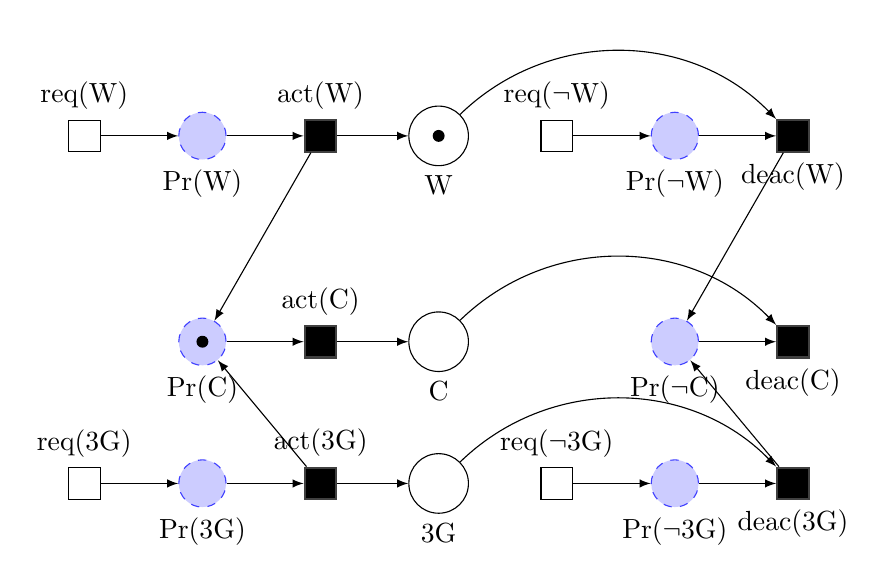
\begin{tikzpicture}[node distance=1.5cm, >=stealth',bend angle=45,auto]
            % WiFi PART

            \node[transition,									label=above:req(W)] (t1) {};
            \node[dplace,right of=t1,tokens=0,label=below:Pr(W)] (p1) {};
            \node[btransition, right of=p1,		label=above:act(W)] (t2) {};
            \node[place, right of=t2,tokens=1,label=below:W] (p2) {};
            \node[transition, right of=p2,		label=above:req($\lnot$W)] (t3) {};
            \node[dplace,right of=t3,tokens=0,label=below:Pr($\lnot$W)] (p3) {};
            \node[btransition, right of=p3,		label=below:deac(W)] (t4) {};

            \path[-latex] (t1) edge node {} (p1);
            \path[-latex] (p1) edge node {} (t2);
            \path[-latex] (t2) edge node {} (p2);
            \path[-latex] (p2) edge[bend left=45] node {} (t4);
            \path[-latex] (t3) edge node {} (p3);
            \path[-latex] (p3) edge node {} (t4);

            % 3G PART

            \node[transition,below =4cm of t1,	label=above:req(3G)] (t5) {};
            \node[dplace, right of=t5,					label=below:Pr(3G)] (p4) {};
            \node[btransition, right of=p4,			label=above:act(3G)] (t6) {};
            \node[place, right of=t6,tokens=0,	label=below:3G] (p5) {};
            \node[transition, right of=p5,			label=above:req($\lnot$3G)] (t7) {};
            \node[dplace, right of=t7,					label=below:Pr($\lnot$3G)] (p6) {};
            \node[btransition, right of=p6,			label=below:deac(3G)] (t8) {};

            \path[-latex] (t5) edge node {} (p4);
            \path[-latex] (p4) edge node {} (t6);
            \path[-latex] (t6) edge node {} (p5);
            \path[-latex] (p5) edge[bend left=45] node {} (t8);
            \path[-latex] (t7) edge node {} (p6);
            \path[-latex] (p6) edge node {} (t8);

            % Connectivity PART

            %\node[transition,below =2cm of t1,	label=above:req(C)] (t9) {};
            \node[dplace,below=2cm of p1,tokens=1,label=below:Pr(C)] (p7) {};
            \node[btransition, right of=p7,			label=above:act(C)] (t10) {};
            \node[place, right of=t10,tokens=0,	label=below:C] (p8) {};
            %\node[transition, right of=p8,			label=above:req($\lnot$C)] (t11) {};
            \node[dplace, below =2cm of p3,					label=below:Pr($\lnot$C)] (p9) {};
            \node[btransition, right of=p9,			label=below:deac(C)] (t12) {};

            %\path[-latex] (t9) edge node {} (p7);
            \path[-latex] (p7) edge node {} (t10);
            \path[-latex] (t10) edge node {} (p8);
            \path[-latex] (p8) edge[bend left=45] node {} (t12);
            %\path[-latex] (t11) edge node {} (p9);
            \path[-latex] (p9) edge node {} (t12);

            % Connections of Contexts

            \path[-latex] (t2) edge node {} (p7);
            \path[-latex] (t6) edge node {} (p7);
            \path[-latex] (t4) edge node {} (p9);
            \path[-latex] (t8) edge node {} (p9);

        \end{tikzpicture}
    \end{figure}
\end{frame}


\begin{frame}[noframenumbering]
    \frametitle{Relation between contexts}
    \begin{figure}[!ht]
        \centering
        \scriptsize
        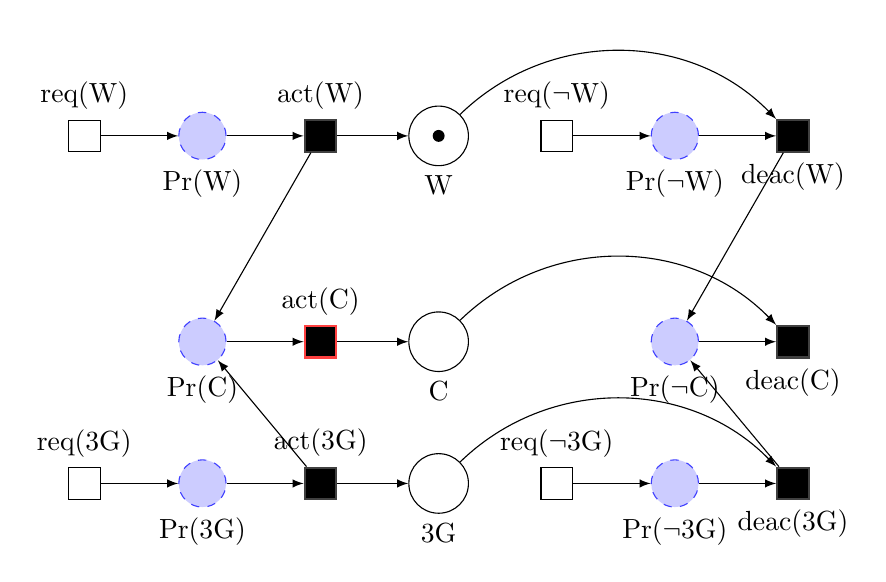
\begin{tikzpicture}[node distance=1.5cm, >=stealth',bend angle=45,auto]
            % WiFi PART

            \node[transition,									label=above:req(W)] (t1) {};
            \node[dplace,right of=t1,tokens=0,label=below:Pr(W)] (p1) {};
            \node[btransition, right of=p1,		label=above:act(W)] (t2) {};
            \node[place, right of=t2,tokens=1,label=below:W] (p2) {};
            \node[transition, right of=p2,		label=above:req($\lnot$W)] (t3) {};
            \node[dplace,right of=t3,tokens=0,label=below:Pr($\lnot$W)] (p3) {};
            \node[btransition, right of=p3,		label=below:deac(W)] (t4) {};

            \path[-latex] (t1) edge node {} (p1);
            \path[-latex] (p1) edge node {} (t2);
            \path[-latex] (t2) edge node {} (p2);
            \path[-latex] (p2) edge[bend left=45] node {} (t4);
            \path[-latex] (t3) edge node {} (p3);
            \path[-latex] (p3) edge node {} (t4);

            % 3G PART

            \node[transition,below =4cm of t1,	label=above:req(3G)] (t5) {};
            \node[dplace, right of=t5,					label=below:Pr(3G)] (p4) {};
            \node[btransition, right of=p4,			label=above:act(3G)] (t6) {};
            \node[place, right of=t6,tokens=0,	label=below:3G] (p5) {};
            \node[transition, right of=p5,			label=above:req($\lnot$3G)] (t7) {};
            \node[dplace, right of=t7,					label=below:Pr($\lnot$3G)] (p6) {};
            \node[btransition, right of=p6,			label=below:deac(3G)] (t8) {};

            \path[-latex] (t5) edge node {} (p4);
            \path[-latex] (p4) edge node {} (t6);
            \path[-latex] (t6) edge node {} (p5);
            \path[-latex] (p5) edge[bend left=45] node {} (t8);
            \path[-latex] (t7) edge node {} (p6);
            \path[-latex] (p6) edge node {} (t8);

            % Connectivity PART

            %\node[transition,below =2cm of t1,	label=above:req(C)] (t9) {};
            \node[dplace, below = 2cm of p1,					label=below:Pr(C)] (p7) {};
            \node[rbtransition, right of=p7,			label=above:act(C)] (t10) {};
            \node[place, right of=t10,tokens=0,	label=below:C] (p8) {};
            %\node[transition, right of=p8,			label=above:req($\lnot$C)] (t11) {};
            \node[dplace, below =2cm of p3,					label=below:Pr($\lnot$C)] (p9) {};
            \node[btransition, right of=p9,			label=below:deac(C)] (t12) {};

            %\path[-latex] (t9) edge node {} (p7);
            \path[-latex] (p7) edge node {} (t10);
            \path[-latex] (t10) edge node {} (p8);
            \path[-latex] (p8) edge[bend left=45] node {} (t12);
            %\path[-latex] (t11) edge node {} (p9);
            \path[-latex] (p9) edge node {} (t12);

            % Connections of Contexts

            \path[-latex] (t2) edge node {} (p7);
            \path[-latex] (t6) edge node {} (p7);
            \path[-latex] (t4) edge node {} (p9);
            \path[-latex] (t8) edge node {} (p9);

        \end{tikzpicture}
    \end{figure}
\end{frame}


\begin{frame}[noframenumbering,plain]
    \begin{figure}[!ht]
        \centering
        \scriptsize
        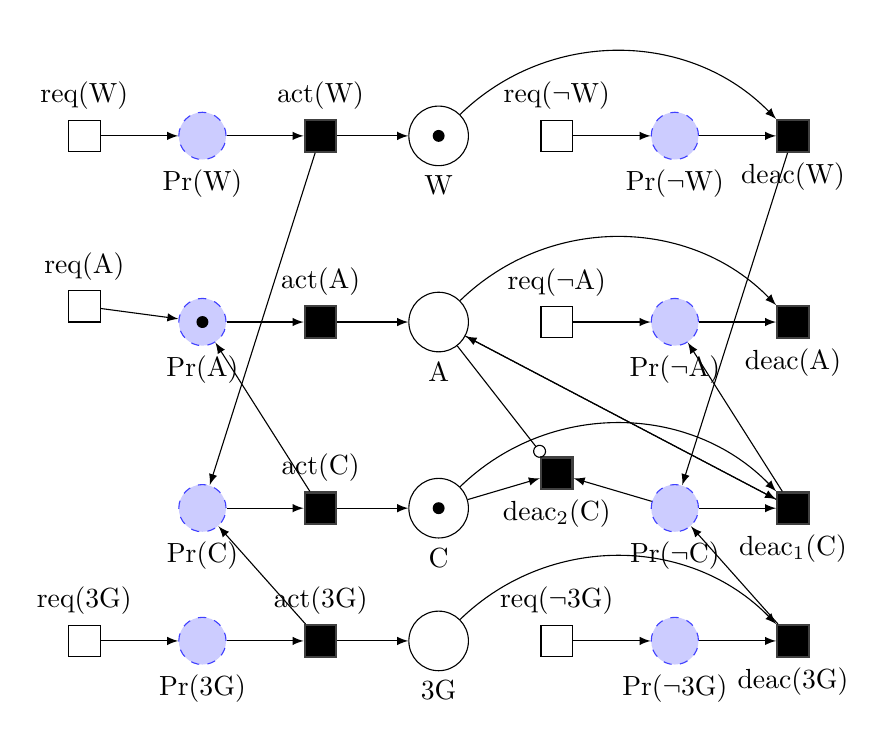
\begin{tikzpicture}[node distance=1.5cm, >=stealth',bend angle=45,auto]
            % WiFi PART

            \node[transition,									label=above:req(W)] (t1) {};
            \node[dplace,right of=t1,tokens=0,label=below:Pr(W)] (p1) {};
            \node[btransition, right of=p1,		label=above:act(W)] (t2) {};
            \node[place, right of=t2,tokens=1,label=below:W] (p2) {};
            \node[transition, right of=p2,		label=above:req($\lnot$W)] (t3) {};
            \node[dplace,right of=t3,tokens=0,label=below:Pr($\lnot$W)] (p3) {};
            \node[btransition, right of=p3,		label=below:deac(W)] (t4) {};

            \path[-latex] (t1) edge node {} (p1);
            \path[-latex] (p1) edge node {} (t2);
            \path[-latex] (t2) edge node {} (p2);
            \path[-latex] (p2) edge[bend left=45] node {} (t4);
            \path[-latex] (t3) edge node {} (p3);
            \path[-latex] (p3) edge node {} (t4);


            % AudioStream PART

            \node[transition,below =1.75cm of t1,  label=above:req(A)] (t13) {};
            \node[dplace, below = 1.75cm of p1,tokens=1, label=below:Pr(A)] (p10) {};
            \node[btransition, right of=p10,    label=above:act(A)] (t14) {};
            \node[place, right of=t14,tokens=0, label=below:A] (p11) {};
            \node[transition, right of=p11,		label=above:req($\lnot$A)] (t15) {};
            \node[dplace, below =1.75cm of p3,     label=below:Pr($\lnot$A)] (p12) {};
            \node[btransition, right of=p12,    label=below:deac(A)] (t16) {};

            \path[-latex] (t13) edge node {} (p10);
            \path[-latex] (p10) edge node {} (t14);
            \path[-latex] (t14) edge node {} (p11);
            \path[-latex] (p11) edge[bend left=45] node {} (t16);
            \path[-latex] (t15) edge node {} (p12);
            \path[-latex] (p12) edge node {} (t16);

            % Connectivity PART

            %\node[transition,below =2cm of t1,	label=above:req(C)] (t9) {};
            \node[dplace, below = 1.75cm of p10,					label=below:Pr(C)] (p7) {};
            \node[btransition, right of=p7,			label=above:act(C)] (t10) {};
            \node[place, right of=t10,tokens=1,	label=below:C] (p8) {};
            %\node[transition, right of=p8,			label=above:req($\lnot$C)] (t11) {};
            \node[dplace, below =1.75cm of p12,					label=below:Pr($\lnot$C)] (p9) {};
            \node[btransition, right of=p9,			label=below:deac$_1$(C)] (t12) {};
            \node[btransition, below=1.5cm of t15,     label=below:deac$_2$(C)] (t17) {};

            %\path[-latex] (t9) edge node {} (p7);
            \path[-latex] (p7) edge node {} (t10);
            \path[-latex] (t10) edge node {} (p8);
            \path[-latex] (p8) edge[bend left=45] node {} (t12);
            %\path[-latex] (t11) edge node {} (p9);
            \path[-latex] (p9) edge node {} (t12);

            % 3G PART

            \node[transition,below =6cm of t1,	label=above:req(3G)] (t5) {};
            \node[dplace, right of=t5,					label=below:Pr(3G)] (p4) {};
            \node[btransition, right of=p4,			label=above:act(3G)] (t6) {};
            \node[place, right of=t6,tokens=0,	label=below:3G] (p5) {};
            \node[transition, right of=p5,			label=above:req($\lnot$3G)] (t7) {};
            \node[dplace, right of=t7,					label=below:Pr($\lnot$3G)] (p6) {};
            \node[btransition, right of=p6,			label=below:deac(3G)] (t8) {};

            \path[-latex] (t5) edge node {} (p4);
            \path[-latex] (p4) edge node {} (t6);
            \path[-latex] (t6) edge node {} (p5);
            \path[-latex] (p5) edge[bend left=45] node {} (t8);
            \path[-latex] (t7) edge node {} (p6);
            \path[-latex] (p6) edge node {} (t8);

            % Connections of Contexts

            \path[-latex] (t2) edge node {} (p7);
            \path[-latex] (t6) edge node {} (p7);
            \path[-latex] (t4) edge node {} (p9);
            \path[-latex] (t8) edge node {} (p9);


            % Connections of Contexts

            \path[-latex] (t10) edge node {} (p10);
            \path[-latex] (t12) edge node {} (p11);
            \path[-latex] (p11) edge node {} (t12);
            \path[-latex] (t12) edge node {} (p12);
            \path[-latex] (p8) edge node {} (t17);
            \path[-latex] (p9) edge node {} (t17);

            \path[-o] (p11) edge node {} (t17);

        \end{tikzpicture}
    \end{figure}
\end{frame}


\begin{frame}[noframenumbering,plain]
    \begin{figure}[!ht]
        \centering
        \scriptsize
        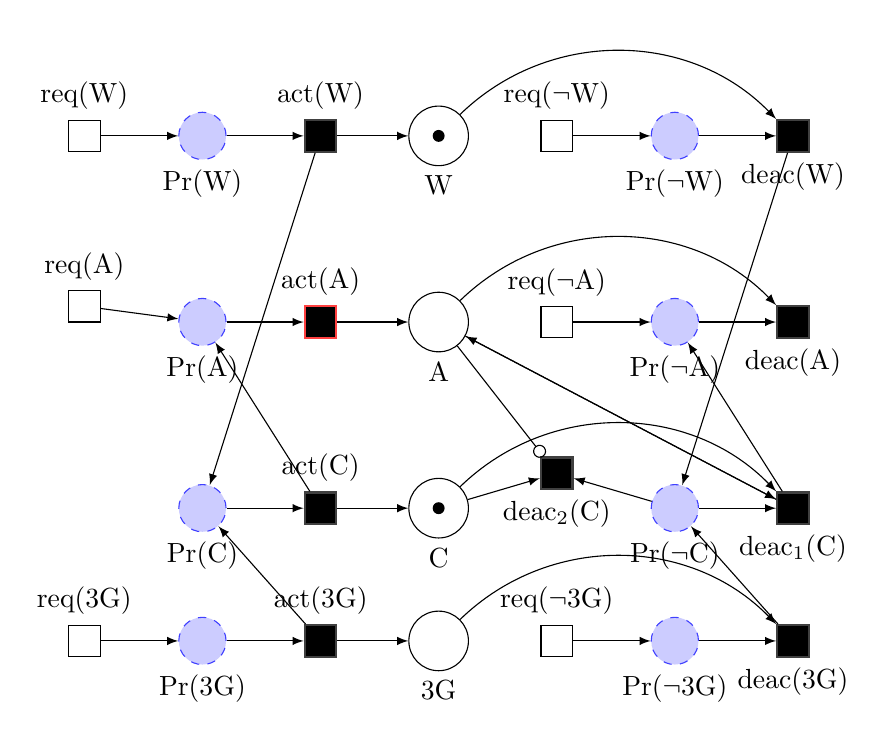
\begin{tikzpicture}[node distance=1.5cm, >=stealth',bend angle=45,auto]
            % WiFi PART

            \node[transition,									label=above:req(W)] (t1) {};
            \node[dplace,right of=t1,tokens=0,label=below:Pr(W)] (p1) {};
            \node[btransition, right of=p1,		label=above:act(W)] (t2) {};
            \node[place, right of=t2,tokens=1,label=below:W] (p2) {};
            \node[transition, right of=p2,		label=above:req($\lnot$W)] (t3) {};
            \node[dplace,right of=t3,tokens=0,label=below:Pr($\lnot$W)] (p3) {};
            \node[btransition, right of=p3,		label=below:deac(W)] (t4) {};

            \path[-latex] (t1) edge node {} (p1);
            \path[-latex] (p1) edge node {} (t2);
            \path[-latex] (t2) edge node {} (p2);
            \path[-latex] (p2) edge[bend left=45] node {} (t4);
            \path[-latex] (t3) edge node {} (p3);
            \path[-latex] (p3) edge node {} (t4);


            % AudioStream PART

            \node[transition,below =1.75cm of t1,  label=above:req(A)] (t13) {};
            \node[dplace, below = 1.75cm of p1,    label=below:Pr(A)] (p10) {};
            \node[rbtransition, right of=p10,    label=above:act(A)] (t14) {};
            \node[place, right of=t14,tokens=0, label=below:A] (p11) {};
            \node[transition, right of=p11,		label=above:req($\lnot$A)] (t15) {};
            \node[dplace, below =1.75cm of p3,     label=below:Pr($\lnot$A)] (p12) {};
            \node[btransition, right of=p12,    label=below:deac(A)] (t16) {};

            \path[-latex] (t13) edge node {} (p10);
            \path[-latex] (p10) edge node {} (t14);
            \path[-latex] (t14) edge node {} (p11);
            \path[-latex] (p11) edge[bend left=45] node {} (t16);
            \path[-latex] (t15) edge node {} (p12);
            \path[-latex] (p12) edge node {} (t16);

            % Connectivity PART

            %\node[transition,below =2cm of t1,	label=above:req(C)] (t9) {};
            \node[dplace, below = 1.75cm of p10,					label=below:Pr(C)] (p7) {};
            \node[btransition, right of=p7,			label=above:act(C)] (t10) {};
            \node[place, right of=t10,tokens=1,	label=below:C] (p8) {};
            %\node[transition, right of=p8,			label=above:req($\lnot$C)] (t11) {};
            \node[dplace, below =1.75cm of p12,					label=below:Pr($\lnot$C)] (p9) {};
            \node[btransition, right of=p9,			label=below:deac$_1$(C)] (t12) {};
            \node[btransition, below=1.5cm of t15,     label=below:deac$_2$(C)] (t17) {};

            %\path[-latex] (t9) edge node {} (p7);
            \path[-latex] (p7) edge node {} (t10);
            \path[-latex] (t10) edge node {} (p8);
            \path[-latex] (p8) edge[bend left=45] node {} (t12);
            %\path[-latex] (t11) edge node {} (p9);
            \path[-latex] (p9) edge node {} (t12);

            % 3G PART

            \node[transition,below =6cm of t1,	label=above:req(3G)] (t5) {};
            \node[dplace, right of=t5,					label=below:Pr(3G)] (p4) {};
            \node[btransition, right of=p4,			label=above:act(3G)] (t6) {};
            \node[place, right of=t6,tokens=0,	label=below:3G] (p5) {};
            \node[transition, right of=p5,			label=above:req($\lnot$3G)] (t7) {};
            \node[dplace, right of=t7,					label=below:Pr($\lnot$3G)] (p6) {};
            \node[btransition, right of=p6,			label=below:deac(3G)] (t8) {};

            \path[-latex] (t5) edge node {} (p4);
            \path[-latex] (p4) edge node {} (t6);
            \path[-latex] (t6) edge node {} (p5);
            \path[-latex] (p5) edge[bend left=45] node {} (t8);
            \path[-latex] (t7) edge node {} (p6);
            \path[-latex] (p6) edge node {} (t8);

            % Connections of Contexts

            \path[-latex] (t2) edge node {} (p7);
            \path[-latex] (t6) edge node {} (p7);
            \path[-latex] (t4) edge node {} (p9);
            \path[-latex] (t8) edge node {} (p9);


            % Connections of Contexts

            \path[-latex] (t10) edge node {} (p10);
            \path[-latex] (t12) edge node {} (p11);
            \path[-latex] (p11) edge node {} (t12);
            \path[-latex] (t12) edge node {} (p12);
            \path[-latex] (p8) edge node {} (t17);
            \path[-latex] (p9) edge node {} (t17);

            \path[-o] (p11) edge node {} (t17);

        \end{tikzpicture}
    \end{figure}
\end{frame}


\begin{frame}[noframenumbering,plain]
    \begin{figure}[!ht]
        \centering
        \scriptsize
        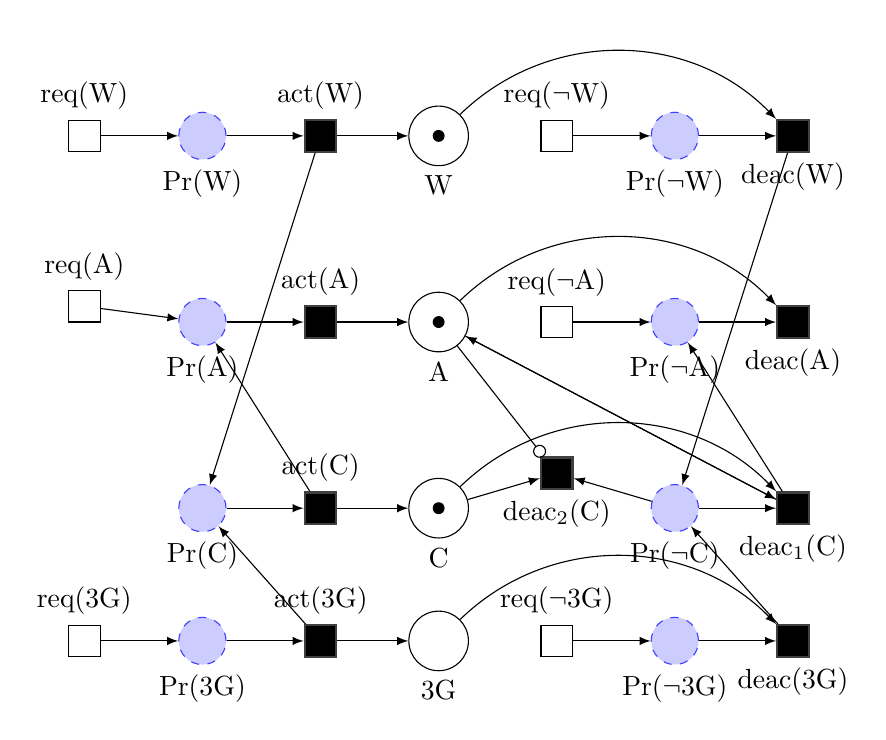
\begin{tikzpicture}[node distance=1.5cm, >=stealth',bend angle=45,auto]
            % WiFi PART

            \node[transition,									label=above:req(W)] (t1) {};
            \node[dplace,right of=t1,tokens=0,label=below:Pr(W)] (p1) {};
            \node[btransition, right of=p1,		label=above:act(W)] (t2) {};
            \node[place, right of=t2,tokens=1,label=below:W] (p2) {};
            \node[transition, right of=p2,		label=above:req($\lnot$W)] (t3) {};
            \node[dplace,right of=t3,tokens=0,label=below:Pr($\lnot$W)] (p3) {};
            \node[btransition, right of=p3,		label=below:deac(W)] (t4) {};

            \path[-latex] (t1) edge node {} (p1);
            \path[-latex] (p1) edge node {} (t2);
            \path[-latex] (t2) edge node {} (p2);
            \path[-latex] (p2) edge[bend left=45] node {} (t4);
            \path[-latex] (t3) edge node {} (p3);
            \path[-latex] (p3) edge node {} (t4);


            % AudioStream PART

            \node[transition,below =1.75cm of t1,  label=above:req(A)] (t13) {};
            \node[dplace, below = 1.75cm of p1,    label=below:Pr(A)] (p10) {};
            \node[btransition, right of=p10,    label=above:act(A)] (t14) {};
            \node[place, right of=t14,tokens=1, label=below:A] (p11) {};
            \node[transition, right of=p11,		label=above:req($\lnot$A)] (t15) {};
            \node[dplace, below =1.75cm of p3,     label=below:Pr($\lnot$A)] (p12) {};
            \node[btransition, right of=p12,    label=below:deac(A)] (t16) {};

            \path[-latex] (t13) edge node {} (p10);
            \path[-latex] (p10) edge node {} (t14);
            \path[-latex] (t14) edge node {} (p11);
            \path[-latex] (p11) edge[bend left=45] node {} (t16);
            \path[-latex] (t15) edge node {} (p12);
            \path[-latex] (p12) edge node {} (t16);

            % Connectivity PART

            %\node[transition,below =2cm of t1,	label=above:req(C)] (t9) {};
            \node[dplace, below = 1.75cm of p10,					label=below:Pr(C)] (p7) {};
            \node[btransition, right of=p7,			label=above:act(C)] (t10) {};
            \node[place, right of=t10,tokens=1,	label=below:C] (p8) {};
            %\node[transition, right of=p8,			label=above:req($\lnot$C)] (t11) {};
            \node[dplace, below =1.75cm of p12,					label=below:Pr($\lnot$C)] (p9) {};
            \node[btransition, right of=p9,			label=below:deac$_1$(C)] (t12) {};
            \node[btransition, below=1.5cm of t15,     label=below:deac$_2$(C)] (t17) {};

            %\path[-latex] (t9) edge node {} (p7);
            \path[-latex] (p7) edge node {} (t10);
            \path[-latex] (t10) edge node {} (p8);
            \path[-latex] (p8) edge[bend left=45] node {} (t12);
            %\path[-latex] (t11) edge node {} (p9);
            \path[-latex] (p9) edge node {} (t12);

            % 3G PART

            \node[transition,below =6cm of t1,	label=above:req(3G)] (t5) {};
            \node[dplace, right of=t5,					label=below:Pr(3G)] (p4) {};
            \node[btransition, right of=p4,			label=above:act(3G)] (t6) {};
            \node[place, right of=t6,tokens=0,	label=below:3G] (p5) {};
            \node[transition, right of=p5,			label=above:req($\lnot$3G)] (t7) {};
            \node[dplace, right of=t7,					label=below:Pr($\lnot$3G)] (p6) {};
            \node[btransition, right of=p6,			label=below:deac(3G)] (t8) {};

            \path[-latex] (t5) edge node {} (p4);
            \path[-latex] (p4) edge node {} (t6);
            \path[-latex] (t6) edge node {} (p5);
            \path[-latex] (p5) edge[bend left=45] node {} (t8);
            \path[-latex] (t7) edge node {} (p6);
            \path[-latex] (p6) edge node {} (t8);

            % Connections of Contexts

            \path[-latex] (t2) edge node {} (p7);
            \path[-latex] (t6) edge node {} (p7);
            \path[-latex] (t4) edge node {} (p9);
            \path[-latex] (t8) edge node {} (p9);


            % Connections of Contexts

            \path[-latex] (t10) edge node {} (p10);
            \path[-latex] (t12) edge node {} (p11);
            \path[-latex] (p11) edge node {} (t12);
            \path[-latex] (t12) edge node {} (p12);
            \path[-latex] (p8) edge node {} (t17);
            \path[-latex] (p9) edge node {} (t17);

            \path[-o] (p11) edge node {} (t17);

        \end{tikzpicture}
    \end{figure}
\end{frame}


\begin{frame}[noframenumbering]
    \frametitle{Relation between contexts}
    \begin{figure}[!ht]
        \centering
        \scriptsize
        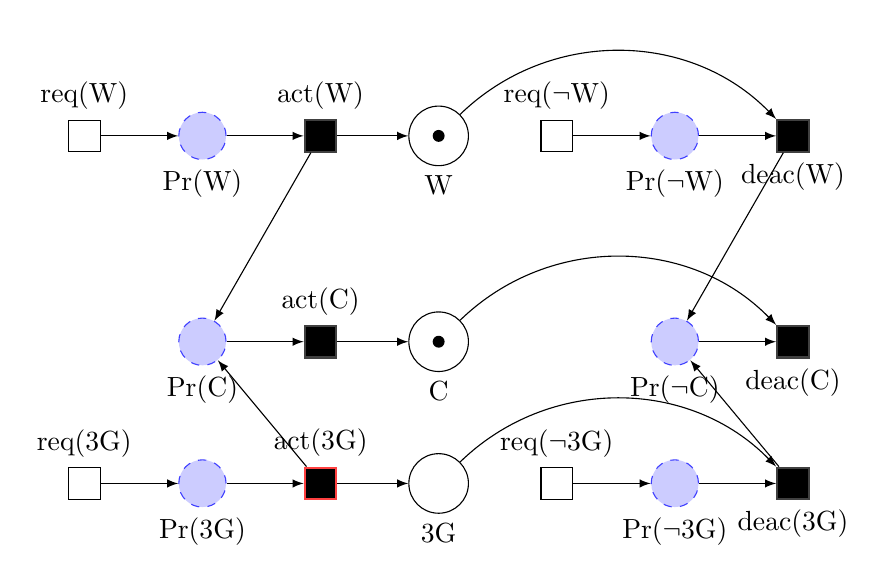
\begin{tikzpicture}[node distance=1.5cm, >=stealth',bend angle=45,auto]
            % WiFi PART

            \node[transition,									label=above:req(W)] (t1) {};
            \node[dplace,right of=t1,tokens=0,label=below:Pr(W)] (p1) {};
            \node[btransition, right of=p1,		label=above:act(W)] (t2) {};
            \node[place, right of=t2,tokens=1,label=below:W] (p2) {};
            \node[transition, right of=p2,		label=above:req($\lnot$W)] (t3) {};
            \node[dplace,right of=t3,tokens=0,label=below:Pr($\lnot$W)] (p3) {};
            \node[btransition, right of=p3,		label=below:deac(W)] (t4) {};

            \path[-latex] (t1) edge node {} (p1);
            \path[-latex] (p1) edge node {} (t2);
            \path[-latex] (t2) edge node {} (p2);
            \path[-latex] (p2) edge[bend left=45] node {} (t4);
            \path[-latex] (t3) edge node {} (p3);
            \path[-latex] (p3) edge node {} (t4);

            % 3G PART

            \node[transition,below =4cm of t1,	label=above:req(3G)] (t5) {};
            \node[dplace, right of=t5,					label=below:Pr(3G)] (p4) {};
            \node[rbtransition, right of=p4,			label=above:act(3G)] (t6) {};
            \node[place, right of=t6,tokens=0,	label=below:3G] (p5) {};
            \node[transition, right of=p5,			label=above:req($\lnot$3G)] (t7) {};
            \node[dplace, right of=t7,					label=below:Pr($\lnot$3G)] (p6) {};
            \node[btransition, right of=p6,			label=below:deac(3G)] (t8) {};

            \path[-latex] (t5) edge node {} (p4);
            \path[-latex] (p4) edge node {} (t6);
            \path[-latex] (t6) edge node {} (p5);
            \path[-latex] (p5) edge[bend left=45] node {} (t8);
            \path[-latex] (t7) edge node {} (p6);
            \path[-latex] (p6) edge node {} (t8);

            % Connectivity PART

            %\node[transition,below =2cm of t1,	label=above:req(C)] (t9) {};
            \node[dplace, below = 2cm of p1,					label=below:Pr(C)] (p7) {};
            \node[btransition, right of=p7,			label=above:act(C)] (t10) {};
            \node[place, right of=t10,tokens=1,	label=below:C] (p8) {};
            %\node[transition, right of=p8,			label=above:req($\lnot$C)] (t11) {};
            \node[dplace, below =2cm of p3,					label=below:Pr($\lnot$C)] (p9) {};
            \node[btransition, right of=p9,			label=below:deac(C)] (t12) {};

            %\path[-latex] (t9) edge node {} (p7);
            \path[-latex] (p7) edge node {} (t10);
            \path[-latex] (t10) edge node {} (p8);
            \path[-latex] (p8) edge[bend left=45] node {} (t12);
            %\path[-latex] (t11) edge node {} (p9);
            \path[-latex] (p9) edge node {} (t12);

            % Connections of Contexts

            \path[-latex] (t2) edge node {} (p7);
            \path[-latex] (t6) edge node {} (p7);
            \path[-latex] (t4) edge node {} (p9);
            \path[-latex] (t8) edge node {} (p9);

        \end{tikzpicture}
    \end{figure}
\end{frame}


\begin{frame}[noframenumbering]
    \frametitle{Relation between contexts}
    \begin{figure}[!ht]
        \centering
        \scriptsize
        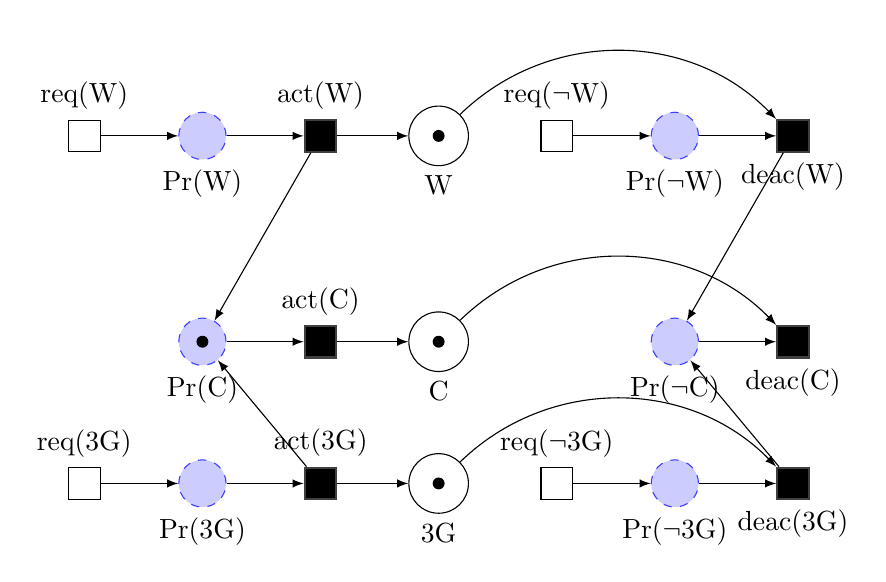
\begin{tikzpicture}[node distance=1.5cm, >=stealth',bend angle=45,auto]
            % WiFi PART

            \node[transition,									label=above:req(W)] (t1) {};
            \node[dplace,right of=t1,tokens=0,label=below:Pr(W)] (p1) {};
            \node[btransition, right of=p1,		label=above:act(W)] (t2) {};
            \node[place, right of=t2,tokens=1,label=below:W] (p2) {};
            \node[transition, right of=p2,		label=above:req($\lnot$W)] (t3) {};
            \node[dplace,right of=t3,tokens=0,label=below:Pr($\lnot$W)] (p3) {};
            \node[btransition, right of=p3,		label=below:deac(W)] (t4) {};

            \path[-latex] (t1) edge node {} (p1);
            \path[-latex] (p1) edge node {} (t2);
            \path[-latex] (t2) edge node {} (p2);
            \path[-latex] (p2) edge[bend left=45] node {} (t4);
            \path[-latex] (t3) edge node {} (p3);
            \path[-latex] (p3) edge node {} (t4);

            % 3G PART

            \node[transition,below =4cm of t1,	label=above:req(3G)] (t5) {};
            \node[dplace, right of=t5,					label=below:Pr(3G)] (p4) {};
            \node[btransition, right of=p4,			label=above:act(3G)] (t6) {};
            \node[place, right of=t6,tokens=1,	label=below:3G] (p5) {};
            \node[transition, right of=p5,			label=above:req($\lnot$3G)] (t7) {};
            \node[dplace, right of=t7,					label=below:Pr($\lnot$3G)] (p6) {};
            \node[btransition, right of=p6,			label=below:deac(3G)] (t8) {};

            \path[-latex] (t5) edge node {} (p4);
            \path[-latex] (p4) edge node {} (t6);
            \path[-latex] (t6) edge node {} (p5);
            \path[-latex] (p5) edge[bend left=45] node {} (t8);
            \path[-latex] (t7) edge node {} (p6);
            \path[-latex] (p6) edge node {} (t8);

            % Connectivity PART

            %\node[transition,below =2cm of t1,	label=above:req(C)] (t9) {};
            \node[dplace,below=2cm of p1,tokens=1,label=below:Pr(C)] (p7) {};
            \node[btransition, right of=p7,			label=above:act(C)] (t10) {};
            \node[place, right of=t10,tokens=1,	label=below:C] (p8) {};
            %\node[transition, right of=p8,			label=above:req($\lnot$C)] (t11) {};
            \node[dplace, below =2cm of p3,					label=below:Pr($\lnot$C)] (p9) {};
            \node[btransition, right of=p9,			label=below:deac(C)] (t12) {};

            %\path[-latex] (t9) edge node {} (p7);
            \path[-latex] (p7) edge node {} (t10);
            \path[-latex] (t10) edge node {} (p8);
            \path[-latex] (p8) edge[bend left=45] node {} (t12);
            %\path[-latex] (t11) edge node {} (p9);
            \path[-latex] (p9) edge node {} (t12);

            % Connections of Contexts

            \path[-latex] (t2) edge node {} (p7);
            \path[-latex] (t6) edge node {} (p7);
            \path[-latex] (t4) edge node {} (p9);
            \path[-latex] (t8) edge node {} (p9);

        \end{tikzpicture}
    \end{figure}
\end{frame}


\begin{frame}[noframenumbering,plain]
    \begin{figure}[!ht]
        \centering
        \scriptsize
        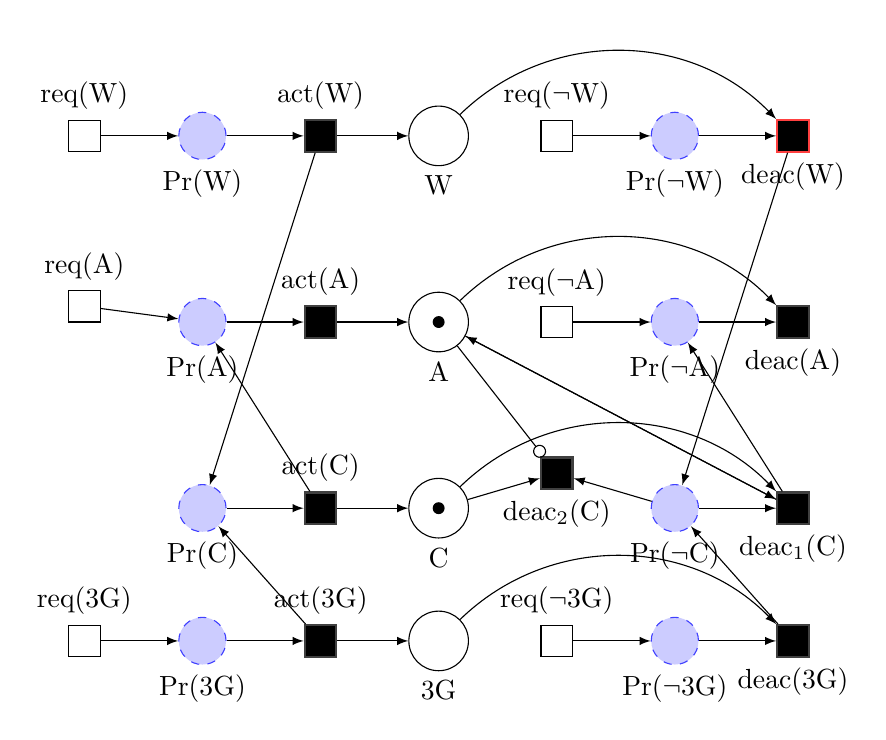
\begin{tikzpicture}[node distance=1.5cm, >=stealth',bend angle=45,auto]
            % WiFi PART

            \node[transition,									label=above:req(W)] (t1) {};
            \node[dplace,right of=t1,tokens=0,label=below:Pr(W)] (p1) {};
            \node[btransition, right of=p1,		label=above:act(W)] (t2) {};
            \node[place, right of=t2,tokens=0,label=below:W] (p2) {};
            \node[transition, right of=p2,		label=above:req($\lnot$W)] (t3) {};
            \node[dplace,right of=t3,tokens=0,label=below:Pr($\lnot$W)] (p3) {};
            \node[rbtransition, right of=p3,		label=below:deac(W)] (t4) {};

            \path[-latex] (t1) edge node {} (p1);
            \path[-latex] (p1) edge node {} (t2);
            \path[-latex] (t2) edge node {} (p2);
            \path[-latex] (p2) edge[bend left=45] node {} (t4);
            \path[-latex] (t3) edge node {} (p3);
            \path[-latex] (p3) edge node {} (t4);


            % AudioStream PART

            \node[transition,below =1.75cm of t1,  label=above:req(A)] (t13) {};
            \node[dplace, below = 1.75cm of p1,    label=below:Pr(A)] (p10) {};
            \node[btransition, right of=p10,    label=above:act(A)] (t14) {};
            \node[place, right of=t14,tokens=1, label=below:A] (p11) {};
            \node[transition, right of=p11,		label=above:req($\lnot$A)] (t15) {};
            \node[dplace, below =1.75cm of p3,     label=below:Pr($\lnot$A)] (p12) {};
            \node[btransition, right of=p12,    label=below:deac(A)] (t16) {};

            \path[-latex] (t13) edge node {} (p10);
            \path[-latex] (p10) edge node {} (t14);
            \path[-latex] (t14) edge node {} (p11);
            \path[-latex] (p11) edge[bend left=45] node {} (t16);
            \path[-latex] (t15) edge node {} (p12);
            \path[-latex] (p12) edge node {} (t16);

            % Connectivity PART

            %\node[transition,below =2cm of t1,	label=above:req(C)] (t9) {};
            \node[dplace, below = 1.75cm of p10,					label=below:Pr(C)] (p7) {};
            \node[btransition, right of=p7,			label=above:act(C)] (t10) {};
            \node[place, right of=t10,tokens=1,	label=below:C] (p8) {};
            %\node[transition, right of=p8,			label=above:req($\lnot$C)] (t11) {};
            \node[dplace, below =1.75cm of p12,					label=below:Pr($\lnot$C)] (p9) {};
            \node[btransition, right of=p9,			label=below:deac$_1$(C)] (t12) {};
            \node[btransition, below=1.5cm of t15,     label=below:deac$_2$(C)] (t17) {};

            %\path[-latex] (t9) edge node {} (p7);
            \path[-latex] (p7) edge node {} (t10);
            \path[-latex] (t10) edge node {} (p8);
            \path[-latex] (p8) edge[bend left=45] node {} (t12);
            %\path[-latex] (t11) edge node {} (p9);
            \path[-latex] (p9) edge node {} (t12);

            % 3G PART

            \node[transition,below =6cm of t1,	label=above:req(3G)] (t5) {};
            \node[dplace, right of=t5,					label=below:Pr(3G)] (p4) {};
            \node[btransition, right of=p4,			label=above:act(3G)] (t6) {};
            \node[place, right of=t6,tokens=0,	label=below:3G] (p5) {};
            \node[transition, right of=p5,			label=above:req($\lnot$3G)] (t7) {};
            \node[dplace, right of=t7,					label=below:Pr($\lnot$3G)] (p6) {};
            \node[btransition, right of=p6,			label=below:deac(3G)] (t8) {};

            \path[-latex] (t5) edge node {} (p4);
            \path[-latex] (p4) edge node {} (t6);
            \path[-latex] (t6) edge node {} (p5);
            \path[-latex] (p5) edge[bend left=45] node {} (t8);
            \path[-latex] (t7) edge node {} (p6);
            \path[-latex] (p6) edge node {} (t8);

            % Connections of Contexts

            \path[-latex] (t2) edge node {} (p7);
            \path[-latex] (t6) edge node {} (p7);
            \path[-latex] (t4) edge node {} (p9);
            \path[-latex] (t8) edge node {} (p9);


            % Connections of Contexts

            \path[-latex] (t10) edge node {} (p10);
            \path[-latex] (t12) edge node {} (p11);
            \path[-latex] (p11) edge node {} (t12);
            \path[-latex] (t12) edge node {} (p12);
            \path[-latex] (p8) edge node {} (t17);
            \path[-latex] (p9) edge node {} (t17);

            \path[-o] (p11) edge node {} (t17);

        \end{tikzpicture}
    \end{figure}
\end{frame}


\begin{frame}[noframenumbering,plain]
    \begin{figure}[!ht]
        \centering
        \scriptsize
        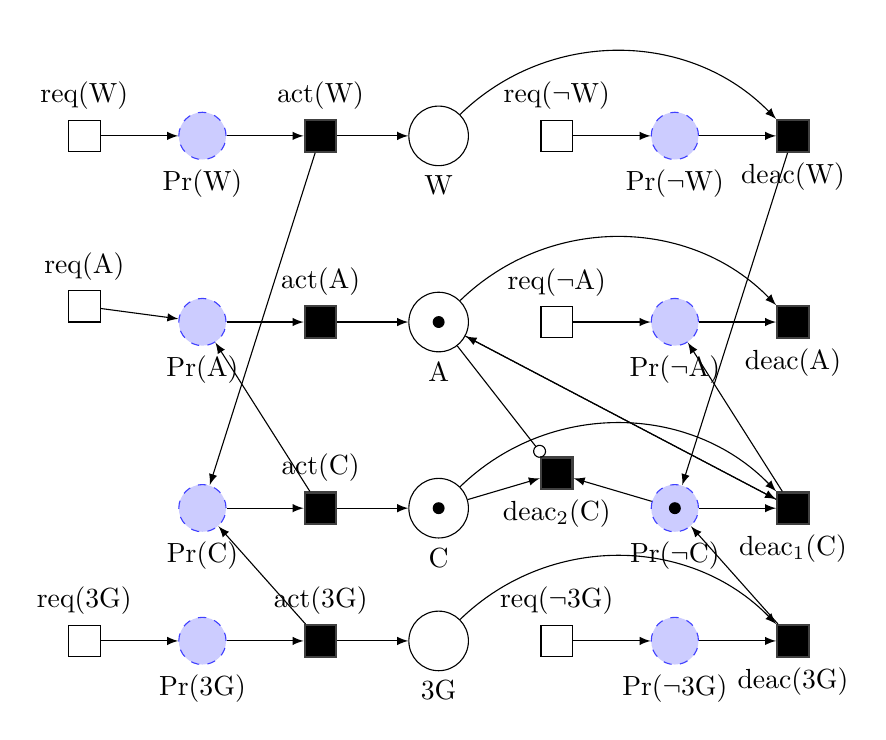
\begin{tikzpicture}[node distance=1.5cm, >=stealth',bend angle=45,auto]
            % WiFi PART

            \node[transition,									label=above:req(W)] (t1) {};
            \node[dplace,right of=t1,tokens=0,label=below:Pr(W)] (p1) {};
            \node[btransition, right of=p1,		label=above:act(W)] (t2) {};
            \node[place, right of=t2,tokens=0,label=below:W] (p2) {};
            \node[transition, right of=p2,		label=above:req($\lnot$W)] (t3) {};
            \node[dplace,right of=t3,tokens=0,label=below:Pr($\lnot$W)] (p3) {};
            \node[btransition, right of=p3,		label=below:deac(W)] (t4) {};

            \path[-latex] (t1) edge node {} (p1);
            \path[-latex] (p1) edge node {} (t2);
            \path[-latex] (t2) edge node {} (p2);
            \path[-latex] (p2) edge[bend left=45] node {} (t4);
            \path[-latex] (t3) edge node {} (p3);
            \path[-latex] (p3) edge node {} (t4);


            % AudioStream PART

            \node[transition,below =1.75cm of t1,  label=above:req(A)] (t13) {};
            \node[dplace, below = 1.75cm of p1,    label=below:Pr(A)] (p10) {};
            \node[btransition, right of=p10,    label=above:act(A)] (t14) {};
            \node[place, right of=t14,tokens=1, label=below:A] (p11) {};
            \node[transition, right of=p11,		label=above:req($\lnot$A)] (t15) {};
            \node[dplace, below =1.75cm of p3,     label=below:Pr($\lnot$A)] (p12) {};
            \node[btransition, right of=p12,    label=below:deac(A)] (t16) {};

            \path[-latex] (t13) edge node {} (p10);
            \path[-latex] (p10) edge node {} (t14);
            \path[-latex] (t14) edge node {} (p11);
            \path[-latex] (p11) edge[bend left=45] node {} (t16);
            \path[-latex] (t15) edge node {} (p12);
            \path[-latex] (p12) edge node {} (t16);

            % Connectivity PART

            %\node[transition,below =2cm of t1,	label=above:req(C)] (t9) {};
            \node[dplace, below = 1.75cm of p10,					label=below:Pr(C)] (p7) {};
            \node[btransition, right of=p7,			label=above:act(C)] (t10) {};
            \node[place, right of=t10,tokens=1,	label=below:C] (p8) {};
            %\node[transition, right of=p8,			label=above:req($\lnot$C)] (t11) {};
            \node[dplace, below =1.75cm of p12,tokens=1,				label=below:Pr($\lnot$C)] (p9) {};
            \node[btransition, right of=p9,			label=below:deac$_1$(C)] (t12) {};
            \node[btransition, below=1.5cm of t15,     label=below:deac$_2$(C)] (t17) {};

            %\path[-latex] (t9) edge node {} (p7);
            \path[-latex] (p7) edge node {} (t10);
            \path[-latex] (t10) edge node {} (p8);
            \path[-latex] (p8) edge[bend left=45] node {} (t12);
            %\path[-latex] (t11) edge node {} (p9);
            \path[-latex] (p9) edge node {} (t12);

            % 3G PART

            \node[transition,below =6cm of t1,	label=above:req(3G)] (t5) {};
            \node[dplace, right of=t5,					label=below:Pr(3G)] (p4) {};
            \node[btransition, right of=p4,			label=above:act(3G)] (t6) {};
            \node[place, right of=t6,tokens=0,	label=below:3G] (p5) {};
            \node[transition, right of=p5,			label=above:req($\lnot$3G)] (t7) {};
            \node[dplace, right of=t7,					label=below:Pr($\lnot$3G)] (p6) {};
            \node[btransition, right of=p6,			label=below:deac(3G)] (t8) {};

            \path[-latex] (t5) edge node {} (p4);
            \path[-latex] (p4) edge node {} (t6);
            \path[-latex] (t6) edge node {} (p5);
            \path[-latex] (p5) edge[bend left=45] node {} (t8);
            \path[-latex] (t7) edge node {} (p6);
            \path[-latex] (p6) edge node {} (t8);

            % Connections of Contexts

            \path[-latex] (t2) edge node {} (p7);
            \path[-latex] (t6) edge node {} (p7);
            \path[-latex] (t4) edge node {} (p9);
            \path[-latex] (t8) edge node {} (p9);


            % Connections of Contexts

            \path[-latex] (t10) edge node {} (p10);
            \path[-latex] (t12) edge node {} (p11);
            \path[-latex] (p11) edge node {} (t12);
            \path[-latex] (t12) edge node {} (p12);
            \path[-latex] (p8) edge node {} (t17);
            \path[-latex] (p9) edge node {} (t17);

            \path[-o] (p11) edge node {} (t17);

        \end{tikzpicture}
    \end{figure}
\end{frame}


\begin{frame}[noframenumbering]
    \frametitle{Relation between contexts}
    \begin{figure}[!ht]
        \centering
        \scriptsize
        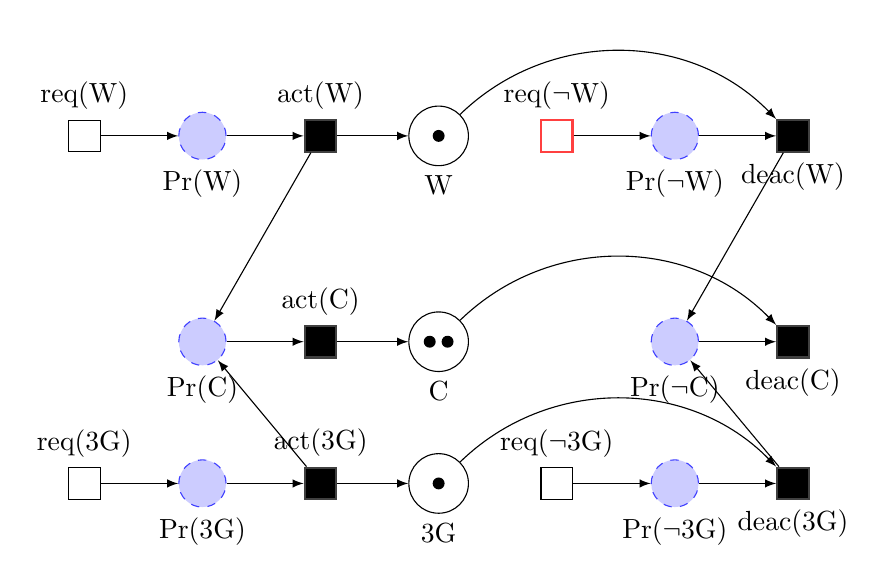
\begin{tikzpicture}[node distance=1.5cm, >=stealth',bend angle=45,auto]
            % WiFi PART

            \node[transition,									label=above:req(W)] (t1) {};
            \node[dplace,right of=t1,tokens=0,label=below:Pr(W)] (p1) {};
            \node[btransition, right of=p1,		label=above:act(W)] (t2) {};
            \node[place, right of=t2,tokens=1,label=below:W] (p2) {};
            \node[rtransition, right of=p2,		label=above:req($\lnot$W)] (t3) {};
            \node[dplace,right of=t3,tokens=0,label=below:Pr($\lnot$W)] (p3) {};
            \node[btransition, right of=p3,		label=below:deac(W)] (t4) {};

            \path[-latex] (t1) edge node {} (p1);
            \path[-latex] (p1) edge node {} (t2);
            \path[-latex] (t2) edge node {} (p2);
            \path[-latex] (p2) edge[bend left=45] node {} (t4);
            \path[-latex] (t3) edge node {} (p3);
            \path[-latex] (p3) edge node {} (t4);

            % 3G PART

            \node[transition,below =4cm of t1,	label=above:req(3G)] (t5) {};
            \node[dplace, right of=t5,					label=below:Pr(3G)] (p4) {};
            \node[btransition, right of=p4,			label=above:act(3G)] (t6) {};
            \node[place, right of=t6,tokens=1,	label=below:3G] (p5) {};
            \node[transition, right of=p5,			label=above:req($\lnot$3G)] (t7) {};
            \node[dplace, right of=t7,					label=below:Pr($\lnot$3G)] (p6) {};
            \node[btransition, right of=p6,			label=below:deac(3G)] (t8) {};

            \path[-latex] (t5) edge node {} (p4);
            \path[-latex] (p4) edge node {} (t6);
            \path[-latex] (t6) edge node {} (p5);
            \path[-latex] (p5) edge[bend left=45] node {} (t8);
            \path[-latex] (t7) edge node {} (p6);
            \path[-latex] (p6) edge node {} (t8);

            % Connectivity PART

            %\node[transition,below =2cm of t1,	label=above:req(C)] (t9) {};
            \node[dplace, below = 2cm of p1,					label=below:Pr(C)] (p7) {};
            \node[btransition, right of=p7,			label=above:act(C)] (t10) {};
            \node[place, right of=t10,tokens=2,	label=below:C] (p8) {};
            %\node[transition, right of=p8,			label=above:req($\lnot$C)] (t11) {};
            \node[dplace, below =2cm of p3,					label=below:Pr($\lnot$C)] (p9) {};
            \node[btransition, right of=p9,			label=below:deac(C)] (t12) {};

            %\path[-latex] (t9) edge node {} (p7);
            \path[-latex] (p7) edge node {} (t10);
            \path[-latex] (t10) edge node {} (p8);
            \path[-latex] (p8) edge[bend left=45] node {} (t12);
            %\path[-latex] (t11) edge node {} (p9);
            \path[-latex] (p9) edge node {} (t12);

            % Connections of Contexts

            \path[-latex] (t2) edge node {} (p7);
            \path[-latex] (t6) edge node {} (p7);
            \path[-latex] (t4) edge node {} (p9);
            \path[-latex] (t8) edge node {} (p9);

        \end{tikzpicture}
    \end{figure}
\end{frame}


\begin{frame}[noframenumbering,plain]
    \begin{figure}[!ht]
        \centering
        \scriptsize
        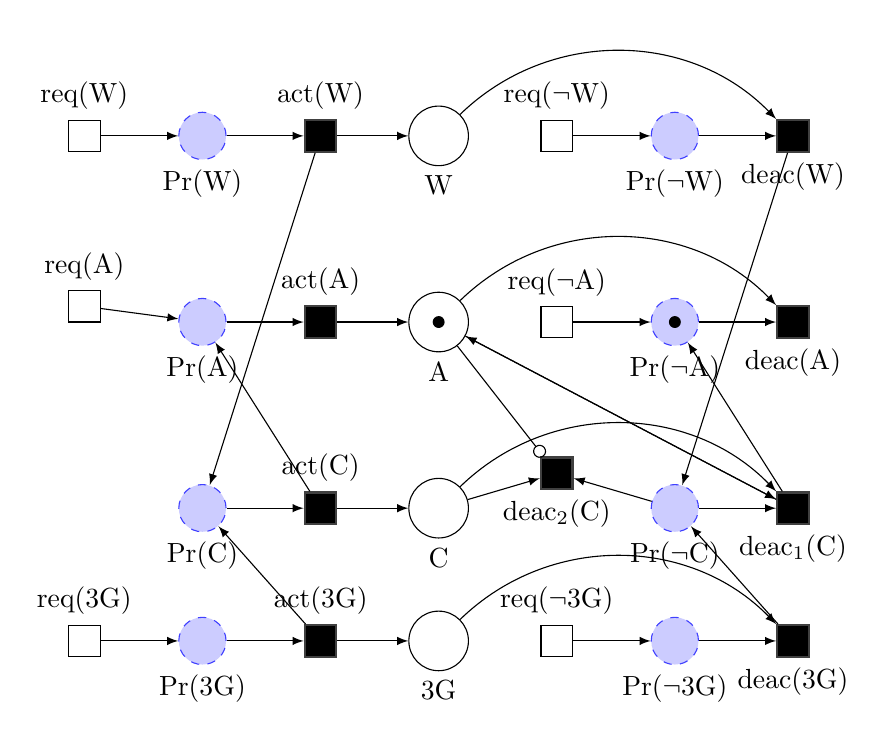
\begin{tikzpicture}[node distance=1.5cm, >=stealth',bend angle=45,auto]
            % WiFi PART

            \node[transition,									label=above:req(W)] (t1) {};
            \node[dplace,right of=t1,tokens=0,label=below:Pr(W)] (p1) {};
            \node[btransition, right of=p1,		label=above:act(W)] (t2) {};
            \node[place, right of=t2,tokens=0,label=below:W] (p2) {};
            \node[transition, right of=p2,		label=above:req($\lnot$W)] (t3) {};
            \node[dplace,right of=t3,tokens=0,label=below:Pr($\lnot$W)] (p3) {};
            \node[btransition, right of=p3,		label=below:deac(W)] (t4) {};

            \path[-latex] (t1) edge node {} (p1);
            \path[-latex] (p1) edge node {} (t2);
            \path[-latex] (t2) edge node {} (p2);
            \path[-latex] (p2) edge[bend left=45] node {} (t4);
            \path[-latex] (t3) edge node {} (p3);
            \path[-latex] (p3) edge node {} (t4);


            % AudioStream PART

            \node[transition,below =1.75cm of t1,  label=above:req(A)] (t13) {};
            \node[dplace, below = 1.75cm of p1,    label=below:Pr(A)] (p10) {};
            \node[btransition, right of=p10,    label=above:act(A)] (t14) {};
            \node[place, right of=t14,tokens=1, label=below:A] (p11) {};
            \node[transition, right of=p11,		label=above:req($\lnot$A)] (t15) {};
            \node[dplace, below =1.75cm of p3,tokens=1,     label=below:Pr($\lnot$A)] (p12) {};
            \node[btransition, right of=p12,    label=below:deac(A)] (t16) {};

            \path[-latex] (t13) edge node {} (p10);
            \path[-latex] (p10) edge node {} (t14);
            \path[-latex] (t14) edge node {} (p11);
            \path[-latex] (p11) edge[bend left=45] node {} (t16);
            \path[-latex] (t15) edge node {} (p12);
            \path[-latex] (p12) edge node {} (t16);

            % Connectivity PART

            %\node[transition,below =2cm of t1,	label=above:req(C)] (t9) {};
            \node[dplace, below = 1.75cm of p10,					label=below:Pr(C)] (p7) {};
            \node[btransition, right of=p7,			label=above:act(C)] (t10) {};
            \node[place, right of=t10,tokens=0,	label=below:C] (p8) {};
            %\node[transition, right of=p8,			label=above:req($\lnot$C)] (t11) {};
            \node[dplace, below =1.75cm of p12,					label=below:Pr($\lnot$C)] (p9) {};
            \node[btransition, right of=p9,			label=below:deac$_1$(C)] (t12) {};
            \node[btransition, below=1.5cm of t15,     label=below:deac$_2$(C)] (t17) {};

            %\path[-latex] (t9) edge node {} (p7);
            \path[-latex] (p7) edge node {} (t10);
            \path[-latex] (t10) edge node {} (p8);
            \path[-latex] (p8) edge[bend left=45] node {} (t12);
            %\path[-latex] (t11) edge node {} (p9);
            \path[-latex] (p9) edge node {} (t12);

            % 3G PART

            \node[transition,below =6cm of t1,	label=above:req(3G)] (t5) {};
            \node[dplace, right of=t5,					label=below:Pr(3G)] (p4) {};
            \node[btransition, right of=p4,			label=above:act(3G)] (t6) {};
            \node[place, right of=t6,tokens=0,	label=below:3G] (p5) {};
            \node[transition, right of=p5,			label=above:req($\lnot$3G)] (t7) {};
            \node[dplace, right of=t7,					label=below:Pr($\lnot$3G)] (p6) {};
            \node[btransition, right of=p6,			label=below:deac(3G)] (t8) {};

            \path[-latex] (t5) edge node {} (p4);
            \path[-latex] (p4) edge node {} (t6);
            \path[-latex] (t6) edge node {} (p5);
            \path[-latex] (p5) edge[bend left=45] node {} (t8);
            \path[-latex] (t7) edge node {} (p6);
            \path[-latex] (p6) edge node {} (t8);

            % Connections of Contexts

            \path[-latex] (t2) edge node {} (p7);
            \path[-latex] (t6) edge node {} (p7);
            \path[-latex] (t4) edge node {} (p9);
            \path[-latex] (t8) edge node {} (p9);


            % Connections of Contexts

            \path[-latex] (t10) edge node {} (p10);
            \path[-latex] (t12) edge node {} (p11);
            \path[-latex] (p11) edge node {} (t12);
            \path[-latex] (t12) edge node {} (p12);
            \path[-latex] (p8) edge node {} (t17);
            \path[-latex] (p9) edge node {} (t17);

            \path[-o] (p11) edge node {} (t17);

        \end{tikzpicture}
    \end{figure}
\end{frame}


\begin{frame}[noframenumbering,plain]
    \begin{figure}[!ht]
        \centering
        \scriptsize
        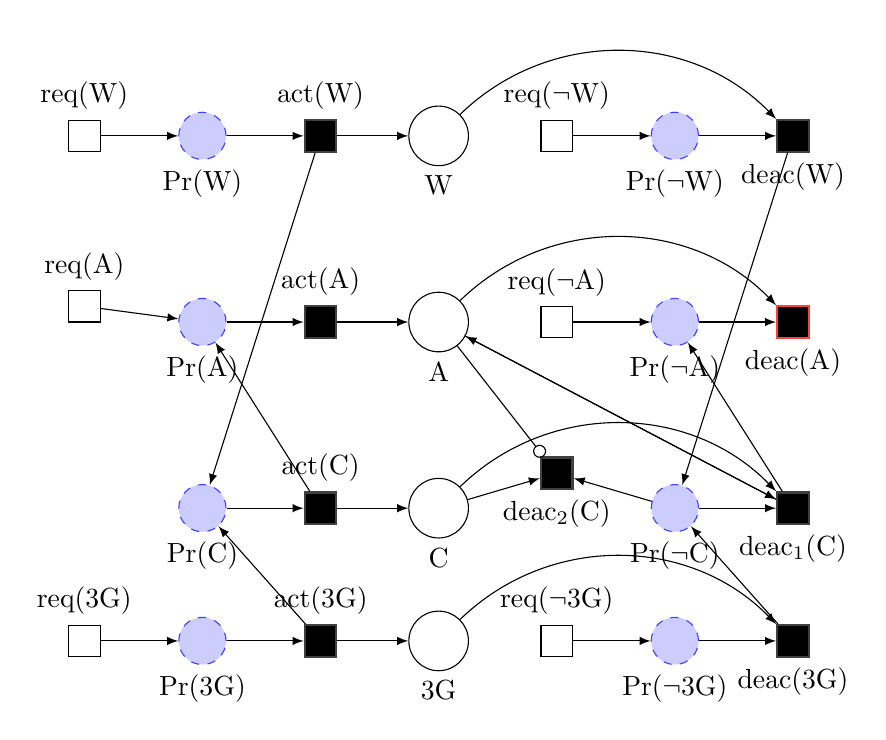
\begin{tikzpicture}[node distance=1.5cm, >=stealth',bend angle=45,auto]
            % WiFi PART

            \node[transition,									label=above:req(W)] (t1) {};
            \node[dplace,right of=t1,tokens=0,label=below:Pr(W)] (p1) {};
            \node[btransition, right of=p1,		label=above:act(W)] (t2) {};
            \node[place, right of=t2,tokens=0,label=below:W] (p2) {};
            \node[transition, right of=p2,		label=above:req($\lnot$W)] (t3) {};
            \node[dplace,right of=t3,tokens=0,label=below:Pr($\lnot$W)] (p3) {};
            \node[btransition, right of=p3,		label=below:deac(W)] (t4) {};

            \path[-latex] (t1) edge node {} (p1);
            \path[-latex] (p1) edge node {} (t2);
            \path[-latex] (t2) edge node {} (p2);
            \path[-latex] (p2) edge[bend left=45] node {} (t4);
            \path[-latex] (t3) edge node {} (p3);
            \path[-latex] (p3) edge node {} (t4);


            % AudioStream PART

            \node[transition,below =1.75cm of t1,  label=above:req(A)] (t13) {};
            \node[dplace, below = 1.75cm of p1,    label=below:Pr(A)] (p10) {};
            \node[btransition, right of=p10,    label=above:act(A)] (t14) {};
            \node[place, right of=t14,tokens=0, label=below:A] (p11) {};
            \node[transition, right of=p11,		label=above:req($\lnot$A)] (t15) {};
            \node[dplace, below =1.75cm of p3,     label=below:Pr($\lnot$A)] (p12) {};
            \node[rbtransition, right of=p12,    label=below:deac(A)] (t16) {};

            \path[-latex] (t13) edge node {} (p10);
            \path[-latex] (p10) edge node {} (t14);
            \path[-latex] (t14) edge node {} (p11);
            \path[-latex] (p11) edge[bend left=45] node {} (t16);
            \path[-latex] (t15) edge node {} (p12);
            \path[-latex] (p12) edge node {} (t16);

            % Connectivity PART

            %\node[transition,below =2cm of t1,	label=above:req(C)] (t9) {};
            \node[dplace, below = 1.75cm of p10,					label=below:Pr(C)] (p7) {};
            \node[btransition, right of=p7,			label=above:act(C)] (t10) {};
            \node[place, right of=t10,tokens=0,	label=below:C] (p8) {};
            %\node[transition, right of=p8,			label=above:req($\lnot$C)] (t11) {};
            \node[dplace, below =1.75cm of p12,					label=below:Pr($\lnot$C)] (p9) {};
            \node[btransition, right of=p9,			label=below:deac$_1$(C)] (t12) {};
            \node[btransition, below=1.5cm of t15,     label=below:deac$_2$(C)] (t17) {};

            %\path[-latex] (t9) edge node {} (p7);
            \path[-latex] (p7) edge node {} (t10);
            \path[-latex] (t10) edge node {} (p8);
            \path[-latex] (p8) edge[bend left=45] node {} (t12);
            %\path[-latex] (t11) edge node {} (p9);
            \path[-latex] (p9) edge node {} (t12);

            % 3G PART

            \node[transition,below =6cm of t1,	label=above:req(3G)] (t5) {};
            \node[dplace, right of=t5,					label=below:Pr(3G)] (p4) {};
            \node[btransition, right of=p4,			label=above:act(3G)] (t6) {};
            \node[place, right of=t6,tokens=0,	label=below:3G] (p5) {};
            \node[transition, right of=p5,			label=above:req($\lnot$3G)] (t7) {};
            \node[dplace, right of=t7,					label=below:Pr($\lnot$3G)] (p6) {};
            \node[btransition, right of=p6,			label=below:deac(3G)] (t8) {};

            \path[-latex] (t5) edge node {} (p4);
            \path[-latex] (p4) edge node {} (t6);
            \path[-latex] (t6) edge node {} (p5);
            \path[-latex] (p5) edge[bend left=45] node {} (t8);
            \path[-latex] (t7) edge node {} (p6);
            \path[-latex] (p6) edge node {} (t8);

            % Connections of Contexts

            \path[-latex] (t2) edge node {} (p7);
            \path[-latex] (t6) edge node {} (p7);
            \path[-latex] (t4) edge node {} (p9);
            \path[-latex] (t8) edge node {} (p9);


            % Connections of Contexts

            \path[-latex] (t10) edge node {} (p10);
            \path[-latex] (t12) edge node {} (p11);
            \path[-latex] (p11) edge node {} (t12);
            \path[-latex] (t12) edge node {} (p12);
            \path[-latex] (p8) edge node {} (t17);
            \path[-latex] (p9) edge node {} (t17);

            \path[-o] (p11) edge node {} (t17);

        \end{tikzpicture}
    \end{figure}
\end{frame}


\begin{frame}[noframenumbering]
    \frametitle{Relation between contexts}
    \begin{figure}[!ht]
        \centering
        \scriptsize
        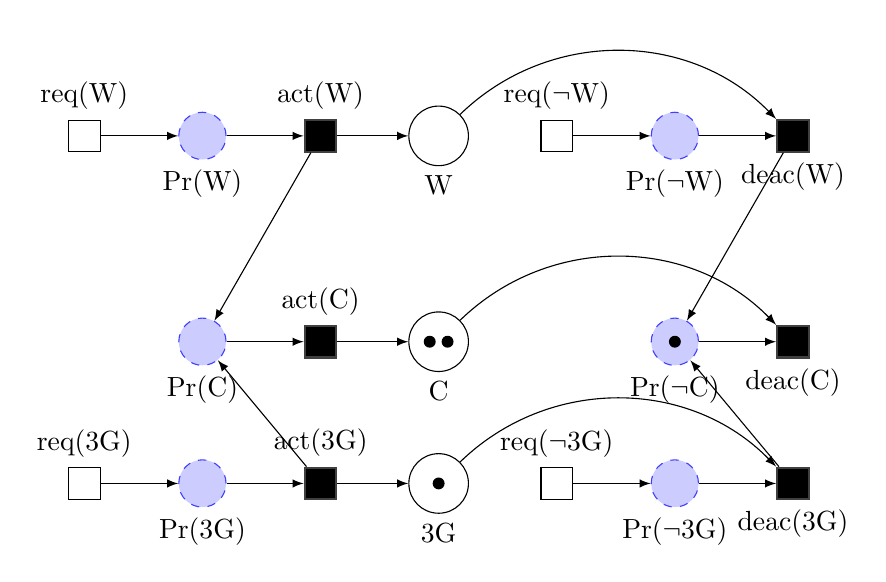
\begin{tikzpicture}[node distance=1.5cm, >=stealth',bend angle=45,auto]
            % WiFi PART

            \node[transition,									label=above:req(W)] (t1) {};
            \node[dplace,right of=t1,tokens=0,label=below:Pr(W)] (p1) {};
            \node[btransition, right of=p1,		label=above:act(W)] (t2) {};
            \node[place, right of=t2,tokens=0,label=below:W] (p2) {};
            \node[transition, right of=p2,		label=above:req($\lnot$W)] (t3) {};
            \node[dplace,right of=t3,tokens=0,label=below:Pr($\lnot$W)] (p3) {};
            \node[btransition, right of=p3,		label=below:deac(W)] (t4) {};

            \path[-latex] (t1) edge node {} (p1);
            \path[-latex] (p1) edge node {} (t2);
            \path[-latex] (t2) edge node {} (p2);
            \path[-latex] (p2) edge[bend left=45] node {} (t4);
            \path[-latex] (t3) edge node {} (p3);
            \path[-latex] (p3) edge node {} (t4);

            % 3G PART

            \node[transition,below =4cm of t1,	label=above:req(3G)] (t5) {};
            \node[dplace, right of=t5,					label=below:Pr(3G)] (p4) {};
            \node[btransition, right of=p4,			label=above:act(3G)] (t6) {};
            \node[place, right of=t6,tokens=1,	label=below:3G] (p5) {};
            \node[transition, right of=p5,			label=above:req($\lnot$3G)] (t7) {};
            \node[dplace, right of=t7,					label=below:Pr($\lnot$3G)] (p6) {};
            \node[btransition, right of=p6,			label=below:deac(3G)] (t8) {};

            \path[-latex] (t5) edge node {} (p4);
            \path[-latex] (p4) edge node {} (t6);
            \path[-latex] (t6) edge node {} (p5);
            \path[-latex] (p5) edge[bend left=45] node {} (t8);
            \path[-latex] (t7) edge node {} (p6);
            \path[-latex] (p6) edge node {} (t8);

            % Connectivity PART

            %\node[transition,below =2cm of t1,	label=above:req(C)] (t9) {};
            \node[dplace, below = 2cm of p1,					label=below:Pr(C)] (p7) {};
            \node[btransition, right of=p7,			label=above:act(C)] (t10) {};
            \node[place, right of=t10,tokens=2,	label=below:C] (p8) {};
            %\node[transition, right of=p8,			label=above:req($\lnot$C)] (t11) {};
            \node[dplace,below=2cm of p3,tokens=1,label=below:Pr($\lnot$C)] (p9) {};
            \node[btransition, right of=p9,			label=below:deac(C)] (t12) {};

            %\path[-latex] (t9) edge node {} (p7);
            \path[-latex] (p7) edge node {} (t10);
            \path[-latex] (t10) edge node {} (p8);
            \path[-latex] (p8) edge[bend left=45] node {} (t12);
            %\path[-latex] (t11) edge node {} (p9);
            \path[-latex] (p9) edge node {} (t12);

            % Connections of Contexts

            \path[-latex] (t2) edge node {} (p7);
            \path[-latex] (t6) edge node {} (p7);
            \path[-latex] (t4) edge node {} (p9);
            \path[-latex] (t8) edge node {} (p9);

        \end{tikzpicture}
    \end{figure}
\end{frame}


\begin{frame}
	\frametitle{Context Petri Nets (CoPN)}

	The previous Petri Net is called a \textbf{Context Petri Net}.
	\bigskip

	There are many more relations between contexts:

	\begin{itemize}
		\item Conjunction dependency relation
		\item Suggestion dependency relation
		\item Requirement dependency relation
		\item Implication dependency relation
		\item \ldots
	\end{itemize}

	There is a corresponding semantic rule for each one in Context Petri Nets!

\end{frame}

\begin{frame}
	\frametitle{Context Petri Nets (CoPN) in practice}

	Subjective-C has built-in language constructs to interact with CoPNs.
	\bigskip

	The CoPN is automatically generated based on the declaration of contexts and
	context dependency relations.
	\bigskip

	Coverability, reachability and liveness properties of Petri Nets can also
	be verified on CoPNs.
\end{frame}

\begin{frame}
	\frametitle{Usefulness of Context Petri Nets}

	CoPN provides a formalism for semantics of context activation and deactivation
	to make sure that subtle errors are unnoticed in context-oriented systems.

	\begin{exampleblock}{In Subjective-C}
		Researchers found an error in the Subjective-C implementation of the
		\textit{implies} relation.\newline

		Two different contexts can imply the activation of the same context. In the
		original definition of the relation in Subjective-C, the deactivation
		of one of those context led to the \textbf{full} deactivation of the
		implied context. This is the kind of subtle errors that you cannot discover if
		you don't have a strong practical formalism that supports relations and multiple
		activations of contexts.
	\end{exampleblock}
\end{frame}

\section{Conclusion}

\begin{frame}
	\frametitle{Conclusion}

	\begin{wideitemize}
		\item \enquote{Standard} Petri Nets are great at modelling context (de)activations
		\pause
		\item But they are not expressive enough for dependency relations
		\pause
		\item Problems can be solved by adding extensions to Petri Nets
		\pause
		\item Context Petri Nets help to verify semantics of context activation
		in context-oriented systems
		\pause
		\item Tools can perform automated model checking given the dependency
		relations
	\end{wideitemize}
\end{frame}

\begin{frame}
	\frametitle{Questions?}

	\begin{center}
		
\includegraphics[height=0.8\paperheight]{questions.png}
	\end{center}
\end{frame}

\begin{frame}[noframenumbering]
	\frametitle{Implication dependency relation}

	\textbf{Example} A system with 2 contexts:

	\begin{itemize}
		\item NLBS context (N)
		\item Positioning context (Pos)
	\end{itemize}

	NLBS provides services that are explicitly used by Positioning context.
	Conversely, if the Positioning is deactivated, the services of the NLBS
	are no longer needed.

	\begin{exampleblock}{Relation type}
		This containment interaction is called an \textit{implication
		dependency relation}, denoted \tikz{\scriptsize
		\node (A) {N}; \node[right of = A] (B) {Pos}; \path[-triangle 45] (A) edge node {} (B);
		}
	\end{exampleblock}
\end{frame}


\begin{frame}[noframenumbering]
	\frametitle{Exclusion dependency relation}

	\begin{figure}[!ht]
		\scriptsize
		\centering
		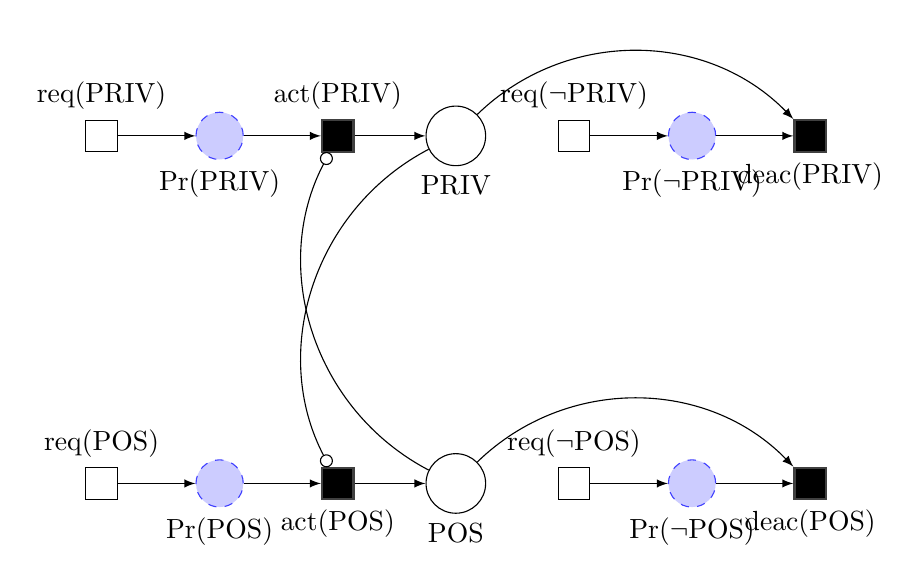
\begin{tikzpicture}[node distance=1.5cm, >=stealth',bend angle=45,auto]
			% PRIV part
			\node[transition,label=above:req(PRIV)] (t1) {};
			\node[dplace,right of=t1,tokens=0,label=below:Pr(PRIV)] (p1) {};
			\node[btransition, right of=p1,		label=above:act(PRIV)] (t2) {};
			\node[place, right of=t2,tokens=0,label=below:PRIV] (p2) {};
			\node[transition, right of=p2,		label=above:req($\lnot$PRIV)] (t3) {};
			\node[dplace,right of=t3,tokens=0,label=below:Pr($\lnot$PRIV)] (p3) {};
			\node[btransition, right of=p3,		label=below:deac(PRIV)] (t4) {};

			\path[-latex] (t1) edge node {} (p1);
			\path[-latex] (p1) edge node {} (t2);
			\path[-latex] (t2) edge node {} (p2);
			\path[-latex] (p2) edge[bend left=45] node {} (t4);
			\path[-latex] (t3) edge node {} (p3);
			\path[-latex] (p3) edge node {} (t4);

			% POS part
			\node[transition,below=4cm of t1,label=above:req(POS)] (t5) {};
			\node[dplace,right of=t5,tokens=0,label=below:Pr(POS)] (p4) {};
			\node[btransition, right of=p4,		label=below:act(POS)] (t6) {};
			\node[place, right of=t6,tokens=0,label=below:POS] (p5) {};
			\node[transition, right of=p5,		label=above:req($\lnot$POS)] (t7) {};
			\node[dplace,right of=t7,tokens=0,label=below:Pr($\lnot$POS)] (p6) {};
			\node[btransition, right of=p6,		label=below:deac(POS)] (t8) {};

			\path[-latex] (t5) edge node {} (p4);
			\path[-latex] (p4) edge node {} (t6);
			\path[-latex] (t6) edge node {} (p5);
			\path[-latex] (p5) edge[bend left=45] node {} (t8);
			\path[-latex] (t7) edge node {} (p6);
			\path[-latex] (p6) edge node {} (t8);

			% Relations between contexts

			\path[-o] (p2) edge[bend right=45] node {} (t6);
			\path[-o] (p5) edge[bend left=45] node {} (t2);
		\end{tikzpicture}
	\end{figure}
\end{frame}


\begin{frame}[noframenumbering]
	\frametitle{Implication dependency relation}

	\textbf{Example} A system with 2 contexts:

	\begin{itemize}
		\item NLBS context (N)
		\item Positioning context (Pos)
	\end{itemize}

	NLBS provides services that are explicitly used by Positioning context.
	Conversely, if the Positioning is deactivated, the services of the NLBS
	are no longer needed.

	\begin{exampleblock}{Relation type}
		This containment interaction is called an \textit{implication
		dependency relation}, denoted \tikz{\scriptsize
		\node (A) {N}; \node[right of = A] (B) {Pos}; \path[-triangle 45] (A) edge node {} (B);
		}
	\end{exampleblock}
\end{frame}


\begin{frame}[noframenumbering]
	\frametitle{Exclusion dependency relation}

	\begin{figure}[!ht]
		\scriptsize
		\centering
		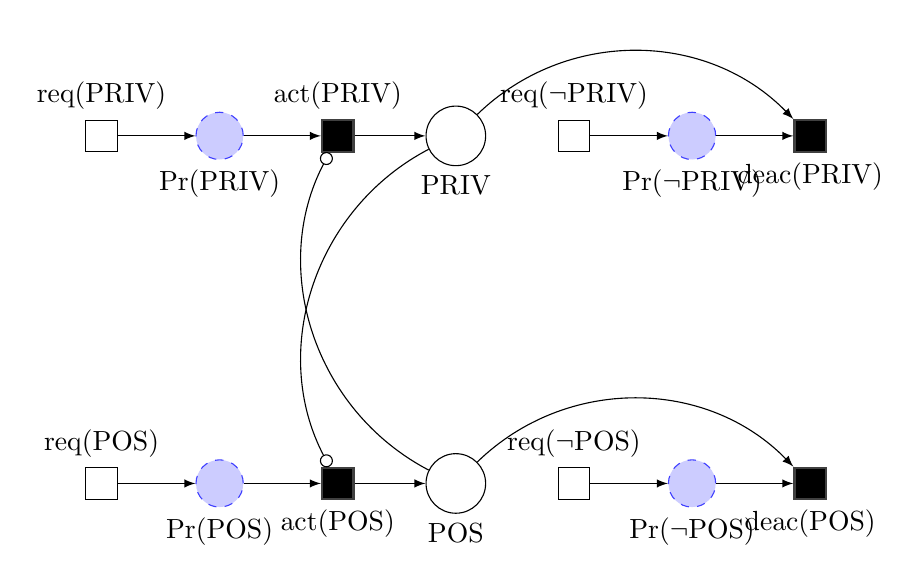
\begin{tikzpicture}[node distance=1.5cm, >=stealth',bend angle=45,auto]
			% PRIV part
			\node[transition,label=above:req(PRIV)] (t1) {};
			\node[dplace,right of=t1,tokens=0,label=below:Pr(PRIV)] (p1) {};
			\node[btransition, right of=p1,		label=above:act(PRIV)] (t2) {};
			\node[place, right of=t2,tokens=0,label=below:PRIV] (p2) {};
			\node[transition, right of=p2,		label=above:req($\lnot$PRIV)] (t3) {};
			\node[dplace,right of=t3,tokens=0,label=below:Pr($\lnot$PRIV)] (p3) {};
			\node[btransition, right of=p3,		label=below:deac(PRIV)] (t4) {};

			\path[-latex] (t1) edge node {} (p1);
			\path[-latex] (p1) edge node {} (t2);
			\path[-latex] (t2) edge node {} (p2);
			\path[-latex] (p2) edge[bend left=45] node {} (t4);
			\path[-latex] (t3) edge node {} (p3);
			\path[-latex] (p3) edge node {} (t4);

			% POS part
			\node[transition,below=4cm of t1,label=above:req(POS)] (t5) {};
			\node[dplace,right of=t5,tokens=0,label=below:Pr(POS)] (p4) {};
			\node[btransition, right of=p4,		label=below:act(POS)] (t6) {};
			\node[place, right of=t6,tokens=0,label=below:POS] (p5) {};
			\node[transition, right of=p5,		label=above:req($\lnot$POS)] (t7) {};
			\node[dplace,right of=t7,tokens=0,label=below:Pr($\lnot$POS)] (p6) {};
			\node[btransition, right of=p6,		label=below:deac(POS)] (t8) {};

			\path[-latex] (t5) edge node {} (p4);
			\path[-latex] (p4) edge node {} (t6);
			\path[-latex] (t6) edge node {} (p5);
			\path[-latex] (p5) edge[bend left=45] node {} (t8);
			\path[-latex] (t7) edge node {} (p6);
			\path[-latex] (p6) edge node {} (t8);

			% Relations between contexts

			\path[-o] (p2) edge[bend right=45] node {} (t6);
			\path[-o] (p5) edge[bend left=45] node {} (t2);
		\end{tikzpicture}
	\end{figure}
\end{frame}


\begin{frame}[noframenumbering]
	\frametitle{Implication dependency relation}

	\textbf{Example} A system with 2 contexts:

	\begin{itemize}
		\item NLBS context (N)
		\item Positioning context (Pos)
	\end{itemize}

	NLBS provides services that are explicitly used by Positioning context.
	Conversely, if the Positioning is deactivated, the services of the NLBS
	are no longer needed.

	\begin{exampleblock}{Relation type}
		This containment interaction is called an \textit{implication
		dependency relation}, denoted \tikz{\scriptsize
		\node (A) {N}; \node[right of = A] (B) {Pos}; \path[-triangle 45] (A) edge node {} (B);
		}
	\end{exampleblock}
\end{frame}


\begin{frame}[noframenumbering]
	\frametitle{Exclusion dependency relation}

	\begin{figure}[!ht]
		\scriptsize
		\centering
		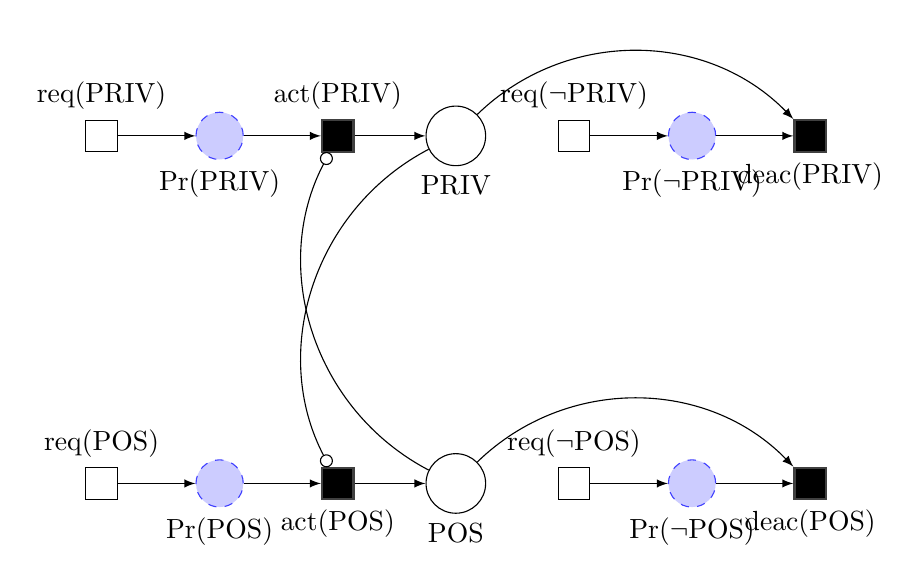
\begin{tikzpicture}[node distance=1.5cm, >=stealth',bend angle=45,auto]
			% PRIV part
			\node[transition,label=above:req(PRIV)] (t1) {};
			\node[dplace,right of=t1,tokens=0,label=below:Pr(PRIV)] (p1) {};
			\node[btransition, right of=p1,		label=above:act(PRIV)] (t2) {};
			\node[place, right of=t2,tokens=0,label=below:PRIV] (p2) {};
			\node[transition, right of=p2,		label=above:req($\lnot$PRIV)] (t3) {};
			\node[dplace,right of=t3,tokens=0,label=below:Pr($\lnot$PRIV)] (p3) {};
			\node[btransition, right of=p3,		label=below:deac(PRIV)] (t4) {};

			\path[-latex] (t1) edge node {} (p1);
			\path[-latex] (p1) edge node {} (t2);
			\path[-latex] (t2) edge node {} (p2);
			\path[-latex] (p2) edge[bend left=45] node {} (t4);
			\path[-latex] (t3) edge node {} (p3);
			\path[-latex] (p3) edge node {} (t4);

			% POS part
			\node[transition,below=4cm of t1,label=above:req(POS)] (t5) {};
			\node[dplace,right of=t5,tokens=0,label=below:Pr(POS)] (p4) {};
			\node[btransition, right of=p4,		label=below:act(POS)] (t6) {};
			\node[place, right of=t6,tokens=0,label=below:POS] (p5) {};
			\node[transition, right of=p5,		label=above:req($\lnot$POS)] (t7) {};
			\node[dplace,right of=t7,tokens=0,label=below:Pr($\lnot$POS)] (p6) {};
			\node[btransition, right of=p6,		label=below:deac(POS)] (t8) {};

			\path[-latex] (t5) edge node {} (p4);
			\path[-latex] (p4) edge node {} (t6);
			\path[-latex] (t6) edge node {} (p5);
			\path[-latex] (p5) edge[bend left=45] node {} (t8);
			\path[-latex] (t7) edge node {} (p6);
			\path[-latex] (p6) edge node {} (t8);

			% Relations between contexts

			\path[-o] (p2) edge[bend right=45] node {} (t6);
			\path[-o] (p5) edge[bend left=45] node {} (t2);
		\end{tikzpicture}
	\end{figure}
\end{frame}


\begin{frame}[noframenumbering]
	\frametitle{Implication dependency relation}

	\textbf{Example} A system with 2 contexts:

	\begin{itemize}
		\item NLBS context (N)
		\item Positioning context (Pos)
	\end{itemize}

	NLBS provides services that are explicitly used by Positioning context.
	Conversely, if the Positioning is deactivated, the services of the NLBS
	are no longer needed.

	\begin{exampleblock}{Relation type}
		This containment interaction is called an \textit{implication
		dependency relation}, denoted \tikz{\scriptsize
		\node (A) {N}; \node[right of = A] (B) {Pos}; \path[-triangle 45] (A) edge node {} (B);
		}
	\end{exampleblock}
\end{frame}


\begin{frame}[noframenumbering]
	\frametitle{Exclusion dependency relation}

	\begin{figure}[!ht]
		\scriptsize
		\centering
		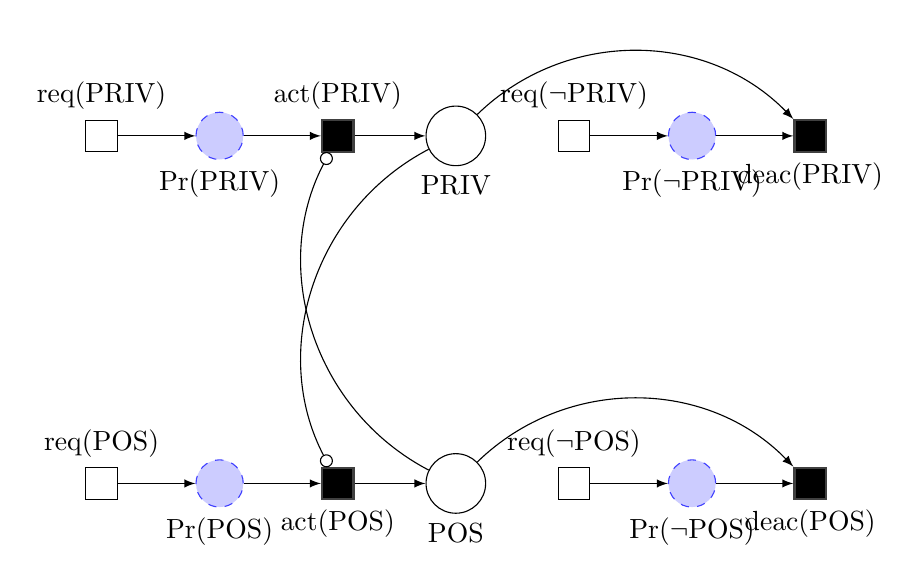
\begin{tikzpicture}[node distance=1.5cm, >=stealth',bend angle=45,auto]
			% PRIV part
			\node[transition,label=above:req(PRIV)] (t1) {};
			\node[dplace,right of=t1,tokens=0,label=below:Pr(PRIV)] (p1) {};
			\node[btransition, right of=p1,		label=above:act(PRIV)] (t2) {};
			\node[place, right of=t2,tokens=0,label=below:PRIV] (p2) {};
			\node[transition, right of=p2,		label=above:req($\lnot$PRIV)] (t3) {};
			\node[dplace,right of=t3,tokens=0,label=below:Pr($\lnot$PRIV)] (p3) {};
			\node[btransition, right of=p3,		label=below:deac(PRIV)] (t4) {};

			\path[-latex] (t1) edge node {} (p1);
			\path[-latex] (p1) edge node {} (t2);
			\path[-latex] (t2) edge node {} (p2);
			\path[-latex] (p2) edge[bend left=45] node {} (t4);
			\path[-latex] (t3) edge node {} (p3);
			\path[-latex] (p3) edge node {} (t4);

			% POS part
			\node[transition,below=4cm of t1,label=above:req(POS)] (t5) {};
			\node[dplace,right of=t5,tokens=0,label=below:Pr(POS)] (p4) {};
			\node[btransition, right of=p4,		label=below:act(POS)] (t6) {};
			\node[place, right of=t6,tokens=0,label=below:POS] (p5) {};
			\node[transition, right of=p5,		label=above:req($\lnot$POS)] (t7) {};
			\node[dplace,right of=t7,tokens=0,label=below:Pr($\lnot$POS)] (p6) {};
			\node[btransition, right of=p6,		label=below:deac(POS)] (t8) {};

			\path[-latex] (t5) edge node {} (p4);
			\path[-latex] (p4) edge node {} (t6);
			\path[-latex] (t6) edge node {} (p5);
			\path[-latex] (p5) edge[bend left=45] node {} (t8);
			\path[-latex] (t7) edge node {} (p6);
			\path[-latex] (p6) edge node {} (t8);

			% Relations between contexts

			\path[-o] (p2) edge[bend right=45] node {} (t6);
			\path[-o] (p5) edge[bend left=45] node {} (t2);
		\end{tikzpicture}
	\end{figure}
\end{frame}


\begin{frame}[noframenumbering]
	\frametitle{Implication dependency relation}

	\textbf{Example} A system with 2 contexts:

	\begin{itemize}
		\item NLBS context (N)
		\item Positioning context (Pos)
	\end{itemize}

	NLBS provides services that are explicitly used by Positioning context.
	Conversely, if the Positioning is deactivated, the services of the NLBS
	are no longer needed.

	\begin{exampleblock}{Relation type}
		This containment interaction is called an \textit{implication
		dependency relation}, denoted \tikz{\scriptsize
		\node (A) {N}; \node[right of = A] (B) {Pos}; \path[-triangle 45] (A) edge node {} (B);
		}
	\end{exampleblock}
\end{frame}


\begin{frame}[noframenumbering]
	\frametitle{Exclusion dependency relation}

	\begin{figure}[!ht]
		\scriptsize
		\centering
		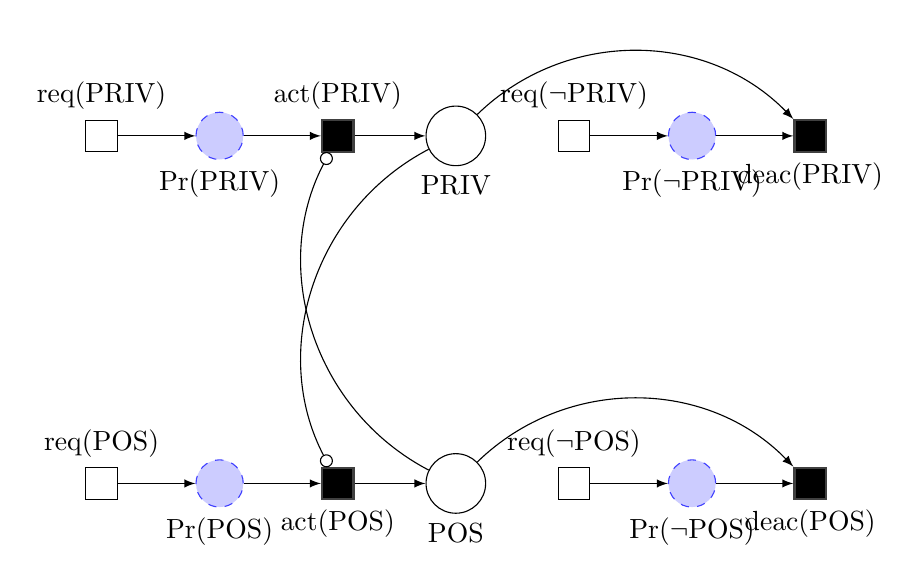
\begin{tikzpicture}[node distance=1.5cm, >=stealth',bend angle=45,auto]
			% PRIV part
			\node[transition,label=above:req(PRIV)] (t1) {};
			\node[dplace,right of=t1,tokens=0,label=below:Pr(PRIV)] (p1) {};
			\node[btransition, right of=p1,		label=above:act(PRIV)] (t2) {};
			\node[place, right of=t2,tokens=0,label=below:PRIV] (p2) {};
			\node[transition, right of=p2,		label=above:req($\lnot$PRIV)] (t3) {};
			\node[dplace,right of=t3,tokens=0,label=below:Pr($\lnot$PRIV)] (p3) {};
			\node[btransition, right of=p3,		label=below:deac(PRIV)] (t4) {};

			\path[-latex] (t1) edge node {} (p1);
			\path[-latex] (p1) edge node {} (t2);
			\path[-latex] (t2) edge node {} (p2);
			\path[-latex] (p2) edge[bend left=45] node {} (t4);
			\path[-latex] (t3) edge node {} (p3);
			\path[-latex] (p3) edge node {} (t4);

			% POS part
			\node[transition,below=4cm of t1,label=above:req(POS)] (t5) {};
			\node[dplace,right of=t5,tokens=0,label=below:Pr(POS)] (p4) {};
			\node[btransition, right of=p4,		label=below:act(POS)] (t6) {};
			\node[place, right of=t6,tokens=0,label=below:POS] (p5) {};
			\node[transition, right of=p5,		label=above:req($\lnot$POS)] (t7) {};
			\node[dplace,right of=t7,tokens=0,label=below:Pr($\lnot$POS)] (p6) {};
			\node[btransition, right of=p6,		label=below:deac(POS)] (t8) {};

			\path[-latex] (t5) edge node {} (p4);
			\path[-latex] (p4) edge node {} (t6);
			\path[-latex] (t6) edge node {} (p5);
			\path[-latex] (p5) edge[bend left=45] node {} (t8);
			\path[-latex] (t7) edge node {} (p6);
			\path[-latex] (p6) edge node {} (t8);

			% Relations between contexts

			\path[-o] (p2) edge[bend right=45] node {} (t6);
			\path[-o] (p5) edge[bend left=45] node {} (t2);
		\end{tikzpicture}
	\end{figure}
\end{frame}


\end{document}
